\documentclass[]{book}


\title{150 Jahre}
\author{Musikgesellschaft Hildisrieden}
\date{1874-2024}

% \usepackage[utf8]{inputenc}
\usepackage{polyglossia}
\usepackage[a4paper, landscape, margin=2cm, twoside, bindingoffset=1cm]{geometry}
\usepackage{multicol}
\usepackage[labelformat=simple]{subfig}
\usepackage{graphicx} % showframe
\usepackage{lipsum}
\usepackage{verbatim}
\usepackage{eso-pic}
\usepackage{fancyhdr}
\usepackage{tikz}
\usepackage{titlesec}
\usepackage{xfrac}
\usepackage{pdfpages}
\usepackage{forloop}
\usepackage[export]{adjustbox}
\usepackage{caption}
\usepackage{csquotes}
\usepackage{threeparttable}
\usepackage{longtable}
\usepackage{floatpag}

\setdefaultlanguage[variant=swiss]{german}

\titleformat{\part}{\normalfont\Huge\bfseries}{}{0em}{}
\titleformat{\chapter}{\normalfont\huge\bfseries}{}{0em}{}
\titleformat{\section}{\normalfont\Large\bfseries}{}{0em}{}
\titleformat{\subsection}{\normalfont\large\bfseries}{}{0em}{}
\titleformat{\subsubsection}{\normalfont\normalsize\bfseries}{}{0em}{}
\titleformat{\paragraph}[runin]{\normalfont\normalsize\bfseries}{}{0em}{}
\titleformat{\subparagraph}[runin]{\normalfont\normalsize\bfseries}{0}{0em}{}

\titlespacing{\chapter}{0em}{0em}{0em}


% redefine plain style (used by first pages of chapters)
\fancypagestyle{plain}{
    \lhead{}
    \fancyhead{}
    \fancyfoot{}
    \renewcommand{\headrulewidth}{0pt}
}

\fancyhf{}
\fancyhead[RO]{\leftmark{}}
\fancyhead[LE]{\leftmark{}}
\fancyfoot[RO]{\thepage}
\fancyfoot[LE]{\thepage}
\pagestyle{fancy}
\floatpagestyle{fancy}

\renewcommand{\headrulewidth}{0pt}
\renewcommand{\chaptermark}[1]{\markboth{#1}{}}
\renewcommand{\sectionmark}[1]{\markboth{#1}{}}
\renewcommand{\subsectionmark}[1]{\markboth{#1}{}}

\renewcommand{\thesubfigure}{\relax}  % Do nothing for the counter »subfigure«


\setlength\columnsep{1cm} %distance between multicolumn columns
\captionsetup{font=small, labelformat=empty} % Bildtitel ohne Kapitelangabe
\captionsetup[subfigure]{justification=justified,singlelinecheck=false}

\newcommand{\groupphoto}[4][0.8]{
    {
            \captionsetup{singlelinecheck=false} % left aligned
            \begin{figure}[!htbp]
                \thisfloatpagestyle{empty}
                \centering
                \def\theight{#1}
                \begin{measuredfigure}
                    \includegraphics[width=0.93\textwidth,height=\theight\textheight, keepaspectratio]{#2}
                \end{measuredfigure}
                \caption{#3}
                \label{#4}
            \end{figure}
        }
}

\newcommand{\portrait}[3][0.8]{
    {
            \captionsetup{singlelinecheck=false} % left aligned
            \begin{figure}[!htbp]
                \def\theight{#1}
                \begin{measuredfigure}
                    \includegraphics[width=0.93\textwidth, height=\theight\textheight, keepaspectratio]{#2}
                    \caption{#3}
                \end{measuredfigure}
            \end{figure}
        }
}
\newcommand{\ConcertProg}[2][0.8]{{
            \begin{figure}[!htbp]
                \centering
                \def\theight{#1}
                \includegraphics[height=\theight\textheight,keepaspectratio]{#2}%
            \end{figure}
        }}

\newcommand{\ConcertProgsTwoVertical}[3][0.485]{{
            \begin{figure}[!htbp]
                \centering
                \def\theight{#1}
                \subfloat{%
                    \includegraphics[height=\theight\textheight,keepaspectratio]{#2}%
                }\\
                \subfloat{%
                    \includegraphics[height=\theight\textheight,keepaspectratio]{#3}%
                }
            \end{figure}
        }}

\newcommand{\ConcertProgsTwoHorizontal}[3][0.485]{{
            \begin{figure}[!htbp]
                \centering
                \def\twidth{#1}
                \subfloat{%
                    \includegraphics[height=\twidth\textwidth,keepaspectratio]{#2}%
                }\hfil
                \subfloat{%
                    \includegraphics[height=\twidth\textwidth,keepaspectratio]{#3}%
                }
            \end{figure}
        }}

\newcommand{\ConcertProgsFourOnPage}[5][0.47]{{
            \begin{figure}[!htbp]
                \centering
                \def\theight{#1}
                \subfloat{%
                    \includegraphics[height=\theight\textheight,keepaspectratio]{#2}%
                }\hfil
                \subfloat{%
                    \includegraphics[height=\theight\textheight,keepaspectratio]{#3}%
                }\\
                \subfloat{%
                    \includegraphics[height=\theight\textheight,keepaspectratio]{#4}%
                }\hfil
                \subfloat{%
                    \includegraphics[height=\theight\textheight,keepaspectratio]{#5}%
                }
            \end{figure}
        }}

\newenvironment{history}{\begin{multicols}{2}}{\end{multicols}} % multicolumn for history text




\begin{document}

\frontmatter
\maketitle


\cleardoublepage

\begin{multicols*}{2}

    % erwinge Text nur in rechter Spalte
    \vphantom{1em}
    \vfill
    \columnbreak

    \section*{Die Entstehung der Chronik}

    Während der ersten Sitzung zur Planung unserer Jubiläumsfeierlichkeiten kam
    das Thema einer Chronik auf den Tisch. Bereits zum 100-jährigen Jubiläum
    wurde eine solche erstellt. Angesichts dessen, und nach einigem Zögern,
    übernahm ich die Aufgabe, eine Chronik für das 150-jährige Bestehen der
    Musikgesellschaft zu verfassen. Damals war mir noch nicht bewusst, wie viel
    Arbeit das bedeutete.

    Wichtige Ereignisse wurden aus den Jahresberichten gefiltert und in eine
    stimmige historische Reihenfolge gebracht. Die älteren, von Hand
    geschriebenen Berichte in den Büchern, boten trotz ihrer teilweise
    anspruchsvollen Lesbarkeit einen wertvollen und vollständigen Einblick. Die
    jüngeren Berichte hingegen, digital gespeichert auf diversen Datenträgern,
    stellten ein anderes Problem dar, da einige Informationen im Laufe der Zeit
    verloren gegangen sind.

    \bigskip

    Um den Schwierigkeiten und Eigenarten von Microsoft Word zu entgehen,
    entschied ich mich für \LaTeX, ein Satzsystem, das vor allem im akademischen
    Bereich für die Erstellung wissenschaftlicher Arbeiten genutzt wird. Die
    Erstellung der Quelltexte erfolgte in einem Texteditor, gefolgt von der
    Übersetzung in ein PDF-Dokument. Um den Fortschritt sicherzustellen,
    speicherte ich regelmässig Versionen in einem \emph{git} Repository und sicherte
    dieses auf GitHub.

    \bigskip

    Diese Chronik ist daher nicht nur ein Zeugnis der reichen Geschichte unserer
    Musikgesellschaft, sondern auch ein Produkt der modernen Technik und einer
    Portion Widerwillen, die schlussendlich in Hingabe umschlug.

    \bigskip

    Ich hoffe, dass dieses Werk die Erinnerungen an unsere vielfältige
    Vergangenheit lebendig hält und kommende Generationen inspiriert.

    \bigskip

    \raggedleft Der Chronist\\
    \raggedleft Martin \enquote{Mumi} Troxler\\
    \raggedleft Sonnerain, Hildisrieden\\

\end{multicols*}


\tableofcontents

\mainmatter

\part{Geschichte}

\chapter{Die ersten 100 Jahre}
Diese Zusammenfassung basiert zum grossen Teil auf der 100-Jahr Chronik, die 1974 von Walter Kaufmann-Lampart erstellt wurde.
\begin{figure}[ht]
    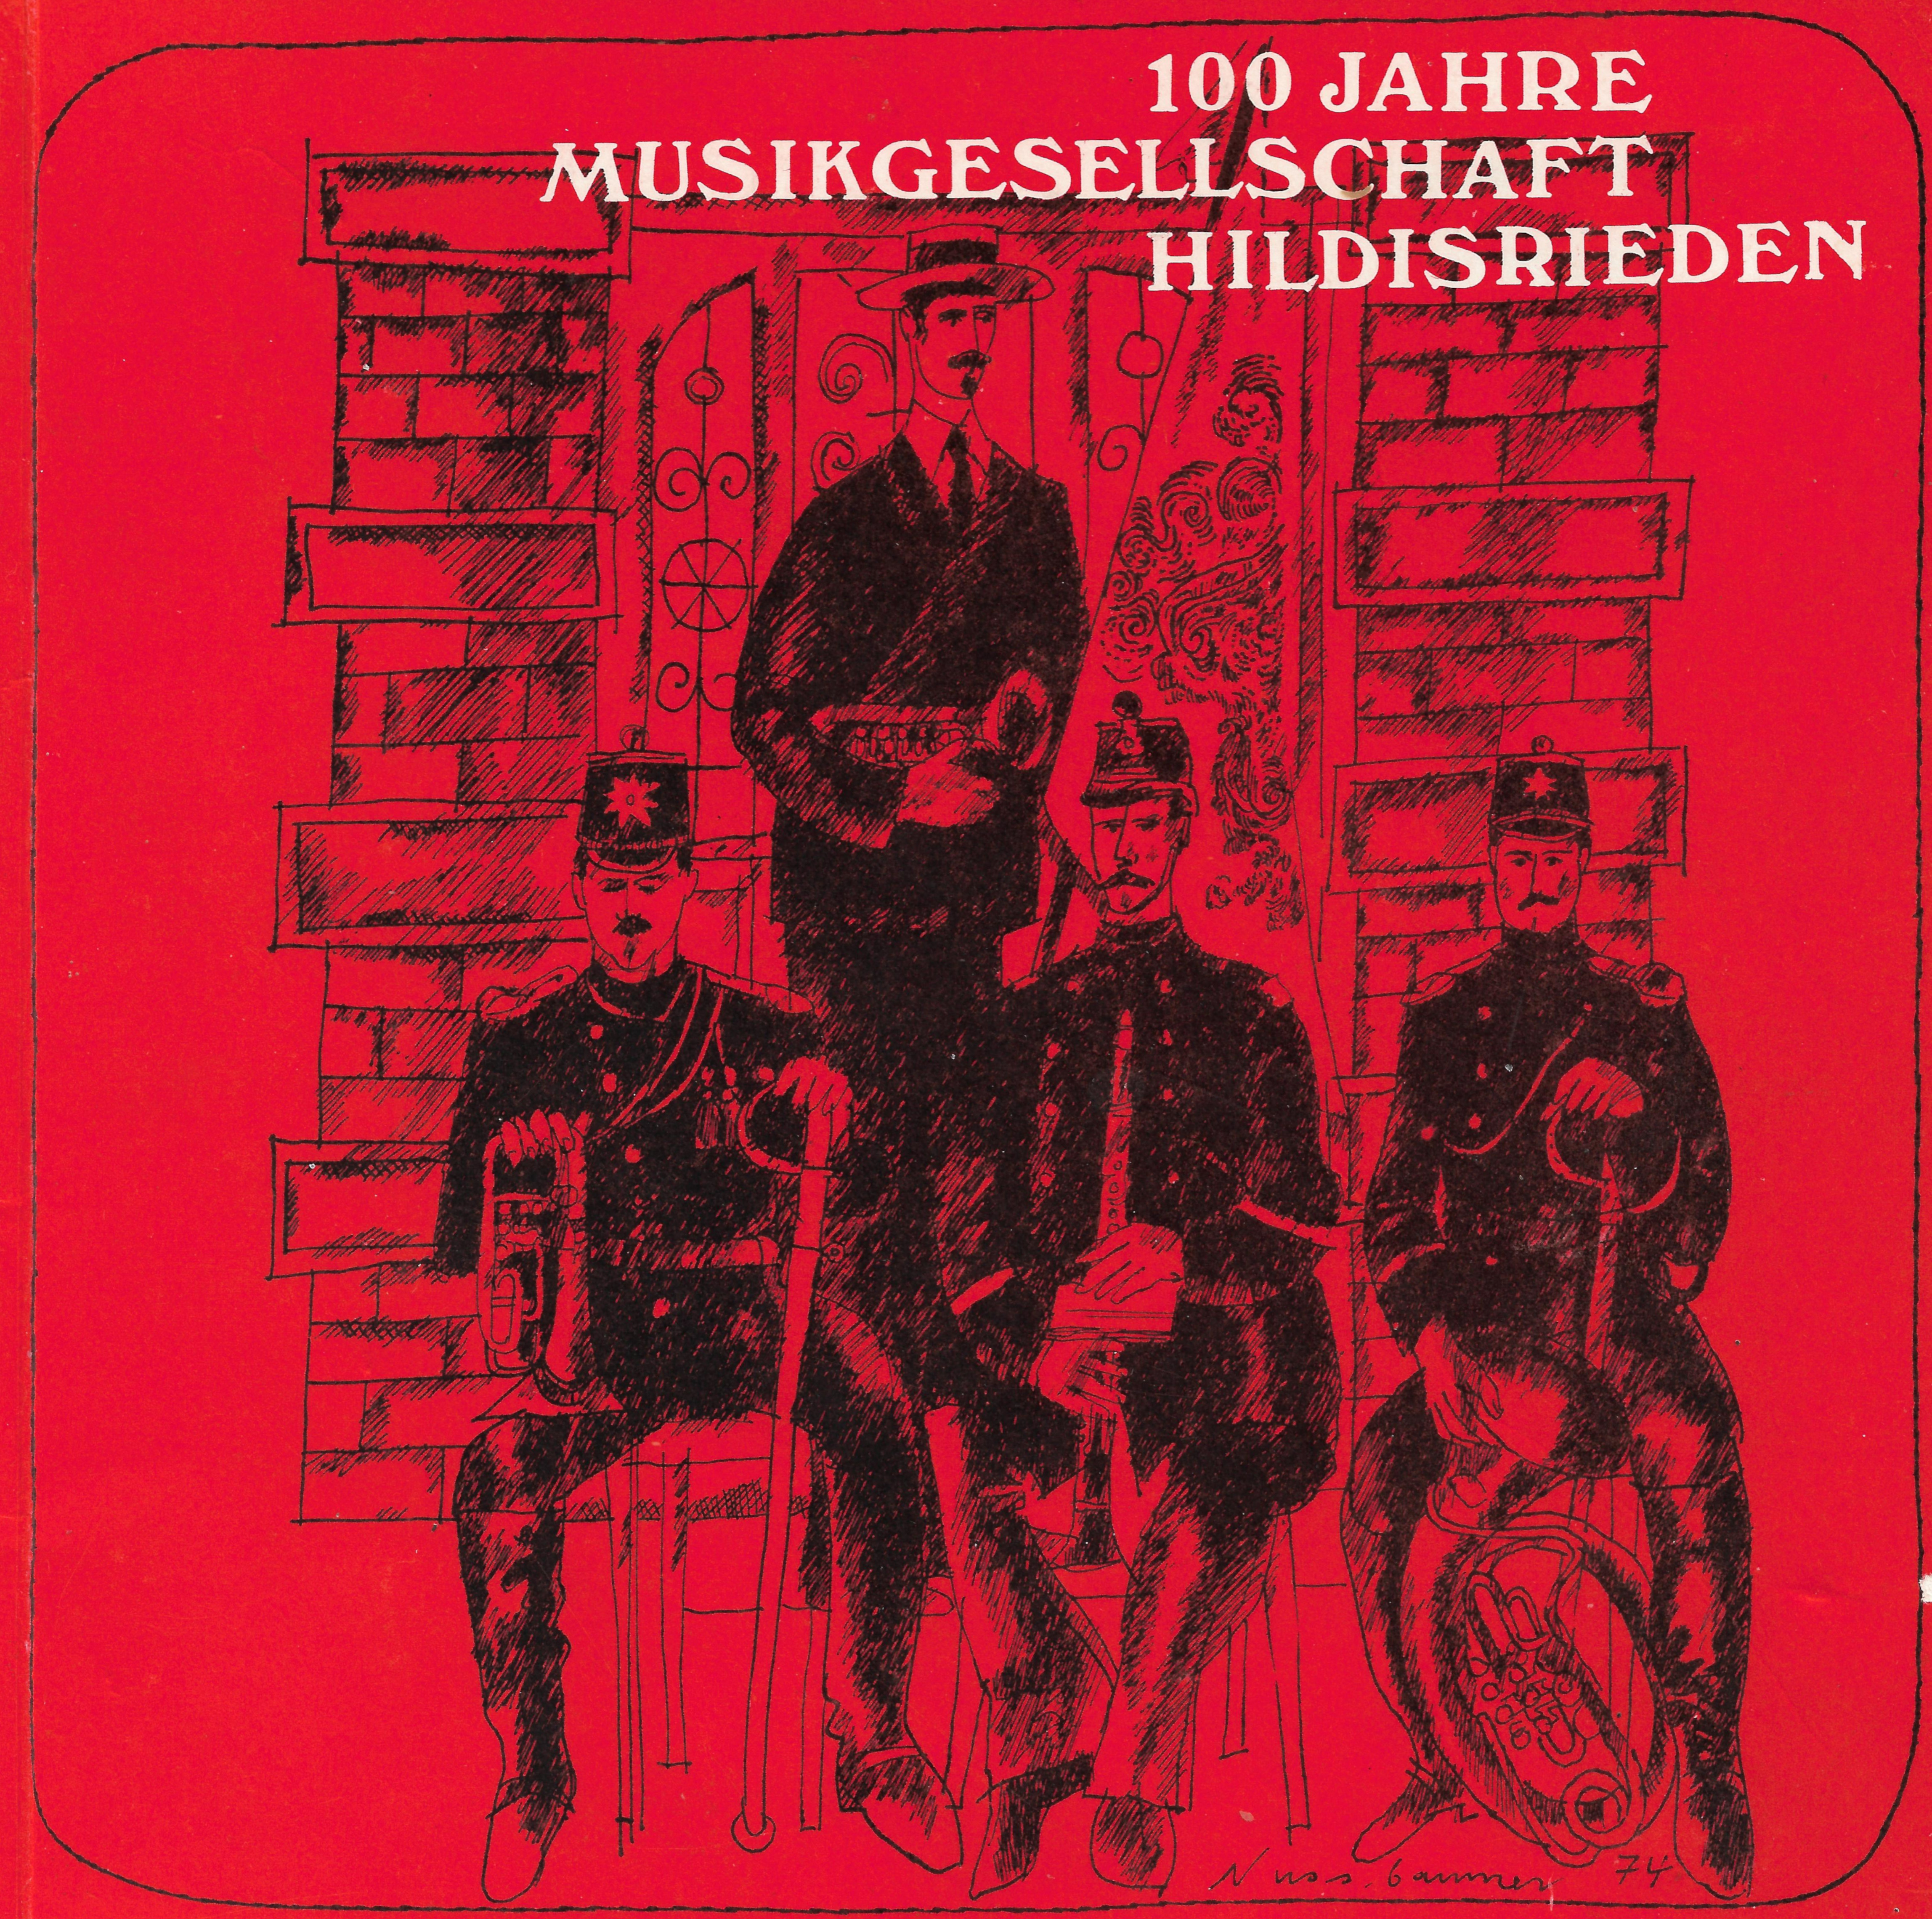
\includegraphics[scale=0.25]{./Cover-100-Jahr-Chronik.jpg}
\end{figure}
\subsection{Vorgeschichte}

\begin{history}

    Der 100. Geburtstag der Musikgesellschaft Hildisrieden gibt uns Gelegenheit,
    viel Wissenswertes und Heimatverbundenes über das musikalische Leben in
    unserem Dorfe zu erzählen. Die Verfassung dieser Erinnerungsschrift über die
    Geschichte und die Taten unserer Musikgesellschaft war keine leichte
    Aufgabe, weil das vorhandene Protokoll erst seit 1912 Auskunft gibt und
    alles vorher Geschehene von verschiedenen Seiten zusammengetragen werden
    musste.

    Dazu leisteten Veteranen und geschichtlich Interessierte wertvolle
    Dienste, was die Nachforschungen sehr erleichterte. Äusserst wertvolle
    Angaben über die Vorgeschichte der Blechmusik Hildisrieden machte uns Peter
    Muff, Lehrer, langjähriger Präsident und Dirigent, welcher alle
    Begebenheiten in ein Notizbuch niederschrieb.

    Diesem entnehmen wir, dass
    schon in den Jahren um 1860 Musikfreunde ein Blechquartett bildeten. Ihrer
    Tätigkeit nach zu schliessen muss angenommen werden, dass sie aus Liebe zur
    Musik und zum eigenen Vergnügen musizierten. In unserer Heimatgemeinde
    Hildisrieden, zwischen Sempacher- und Baldeggersee liegend, inmitten
    prächtiger Matten und Wiesen, wohl bestellter Äcker und gepflegter
    Obstgärten, ist eines erhalten geblieben, was damals schon unsere Ahnen für
    gut und recht fanden, nämlich die MUSIK.

    Musik in Freud und Leid, zu Tanz und Unterhaltung! So spielten sie an
    Weihnachten und Neujahr im Dorfe und auf den Gehöften von Schopfen,
    Traselingen, Holzmatt, Ohmenlingen und Oele.

    Musik ist eine dem Menschen von Natur aus angeborene Sache. Diese wurde im
    Laufe des Jahrhunderts in besonderem Masse in Hildisrieden gehegt und
    gepflegt. Bekanntlich vererben und erhalten sich Sitten und Bräuche in einem
    kleinen Dorfe von Generation zu Generation. So stellt man fest, dass die
    Familien Disler, Estermann und Troxler während drei Generationen das
    musikalische Leben in Hildisrieden prägten.

\end{history}


\section*{1874-1900}
\input{./chap/1874-1900/Gruendung.tex}
\begin{multicols}{2}

    \subsection{Statuten vom 25. März 1876}

    Es hat sich in der Gemeinde Hildisrieden unter obigem
    Datum eine neue Musikgesellschaft gebildet, welche
    den Mitgliedern zum besseren Gedeihen der Gesellschaft
    folgende Bedingungen festgesetzt:

    \S1
    Jedes Mitglied soll, wenn möglich, lange bei der Gesellschaft
    verbleiben und dieselbe fördern.

    \S2
    Die Gesellschaft bildet sich nicht nur zum Schein, sie
    will auch etwas erlernen, um sich auch produzieren zu
    können, daher verpflichtet sich jedes Mitglied, an den
    vorhergesagten Proben zu erscheinen.

    \S3
    Zum Bestimmen der Proben, sowie zum Dirigieren
    wählt die Gesellschaft einen Kapellmeister.

    \S4
    Wer an der Probe 20 Minuten zu spät erscheint, der
    wird um 20 Cts., wer eine halbe Stunde zu spät kommt
    um 30, und wer gar nicht erscheint, um 50 Cts. bestraft.

    \S5
    Wenn es gewisse Umstände verlangen, so ist der Kapellmeister
    berechtigt, festzustellen, was von den Mitgliedern bis zur
    nächsten Probe gelernt werden soll.

    \S6
    Wird etwas nicht gelernt und man sieht, dass es flissentlich
    nicht geschehen ist, so ist der Betreffende in
    eine Strafe von 30 Cts. verfallen, die jedoch auch erhöht werden
    kann bis auf einen Franken.

    \S7
    Kann sich ein Mitglied mit der Gesellschaft nicht mehr
    vertragen, so steht es dieser frei, das Mitglied auszuschliessen,

    \S8
    Tritt ein Mitglied nach eigener Willkür aus der Gesellschaft,
    so hat es eine Entschädigung von 20 Fr. zu entrichten.

    \S9
    Wer nicht mehr an den Proben erscheint, der schliesst
    sich von selbst aus der Gesellschaft und die Entschädigung folgt.
    Die Gelder, Strafgelder sowie andere, sind vom Präsidenten einzuziehen
    und er hat die Pflicht, zu besorgen und am Ende des Jahres oder wenn
    es die Gesellschaft verlangt, genaue Rechnung abzugeben.

    \S10 |
    Was Instrumente anbetrifft, so hat jedes Mitglied das
    seinige selbst anzuschaffen und zu besorgen. Ein
    schlechtes Instrument wird nicht geduldet.

    \S12
    Wenn 2/3 der Mitglieder einen Ausmarsch verlangen,
    und ein Mitglied will oder kann nicht kommen, so hat
    es dieser sofort dem Kapellmeister anzuzeigen, sonst
    ist es in eine Strafe von drei Fr. verfallen. Die Gesellschaft
    zieht dann eine andere Person zu und das betreffende Mitglied
    hat selbe zu entschädigen und ihr sein Instrument zu leihen.

    \S13
    Jedes Mitglied soll sich dem Befehl des Kapellmeisters
    und Präsidenten fügen soweit ihnen die Gesellschaft
    das Recht in die Hand gelegt hat.

    \S14
    Kommt etwas vor, das in dem Rechte dieser zwei Personen liegt,
    so wird die Gesellschaft angefragt, und es wird abgestimmt.

    \S15
    Tritt ein neues Mitglied in die Gesellschaft, so hat es eine
    Eintrittszahlung von zehn Fr. zu entrichten und sein Instrument
    anzuschaffen. Dann tritt es in die gleichen Rechte wie die andern Mitglieder.

    \S16
    Auch diese, so wie alle andern Gelder werden vom Präsidenten
    bezogen und er hat am Ende des Jahres genaue Rechnung abzugeben,
    wonach die Gelder unter die Mitglieder gleichmässig verteilt werden.
    Am Ende Jahres hat jedoch ein Saldo von 20 Fr. in der Kasse
    zu bleiben, das zum Anschaffen neuer Musikstücke
    aufs folgende Jahr verwendet wird.

    \S17
    Die Musikstücke werden vom Präsidenten oder Kapellmeister bestellt, sie
    haben jedoch die Gesellschaft zuerst anzufragen.

    \S18
    Die bestellten Stücke werden vom Präsidenten bezahlt
    und er hat darüber Rechnung zu geben.

    \S19
    Würde es der Fall sein, dass ein Mitglied stürbe, so
    würde die Gesellschaft für dasselbe einen angemessenen
    Gottesdienst halten lassen,

    \S20
    Wer bei der Musik sein will, muss auch in die Gesellschaft treten.

    \S21
    Die Gesellschaft wählt einen Vorstand von 3 Mit-
    gliedern: Kapellmeister, Präsident und Schreiber auf
    eine Amtsdauer von zwei Jahren.

    \S22
    Der Schreiber schreibt die Stücke und alles, was die
    Gesellschaft beschlägt, wofür er angemessen entschädigt
    wird.

    \S23
    Als Entschuldigung wird in allen Fällen nur Krankheit oder Militärdienst angenommen.

    \S24
    Jedes Mitglied hat sich eigenhändig zu unterzeichnen.\\


\end{multicols}

\begin{history}

    \subsection{1875-1900}

    Die Wiegenjahre brachten der Musikgesellschaft Hildisrieden
    abwechslungsreiche Begebenheiten.

    Die Hauptbetätigung blieb weiterhin das Konzertieren in Form von Ständchen
    und Ausmärschen, in und ausserhalb der Gemeinde. So treffen wir die
    Musikgesellschaft 1882 im Emmenbaum anlässlich einer Theateraufführung und
    1887 beritten am Auffahrtsumritt in Sempach. Die Entschädigung, welche die
    Musikgesellschaft von der Kirchenverwaltung Sempach erhielt, betrug immerhin
    45 Franken. Ein Gesuch, den Auffahrtsumritt abwechslungsweise mit der
    Musikgesellschaft Sempach alle drei Jahre bestreiten zu dürfen, wurde von
    der Kirchenverwaltung abgelehnt. Was unseren Musikanten in den 1890er Jahren
    vorgeworfen werden konnte, war der Mangel an Ordnung    und Disziplin. Wohl
    hatte man 1884 neue Statuten aufgestellt und neue Strafbestimmungen
    festgesetzt; diese sind aber nicht von allen befolgt worden. Diese unruhigen
    Vereinsjahre, fünf an der Zahl, hatten zur Folge, dass man mit dem Gedanken
    spielte, die Musikgesellschaft aufzulösen oder sich den gegebenen Statuten
    zu fügen.

    Man fand sich hin und wieder zusammen und kam ebenso schnell wieder
    auseinander, bis schliesslich die Vernunft siegte. Ein weiterer Grund, der
    den Zusammenhang des Vereins trübte, war der kleine finanzielle Beitrag der
    Gemeinde. Jährlich 20 Franken waren wirklich kein grosses Honorar, wenn man
    bedenkt, dass jeder Musikant sein Instrument selbst zu beschaffen und die
    Musikgesellschaft an sämtlichen Prozessionen teilzunehmen hatte.

    Im Jahre 1899 wurde das Restaurant Kreuz eröffnet und der Saal im Löwen
    eingeweiht. Die Einladung zu diesen Festen fügte das schwache Gebilde wieder
    zusammen.

    Die Statuten von 1874 und 1884 erneuert, haben 10 Mitglieder unterzeichnet.
    Es sind: Silvester Schnieper, Josef Wolf, Leonz Geisshüsler, Silvester
    Disler, Josef Disler, Peter Troxler, Peter Muff, Rudolf Bühlmann, Josef Wolf
    und Niklaus Süess.

    Weitere Einnahmen wurden mit dem \enquote{Umblasen}  während der
    Weihnachtszeit in der Gemeinde erzielt. Vor den Häusern wurde jeweils
    musiziert, wofür die Musik-freundlichen Bewohner eine Geldgabe spendeten. Im
    Jahre 1886 brachte der Verein auf diese Weise Fr. 259.60 zusammen. Bei
    kaltem Wetter war das Musizieren kein Vergnügen, denn öfters froren die
    Ventile ein und mussten durch Einhauchen wieder beweglich gemacht werden.
    Gerne wurde dann die Einladung angenommen, ins Haus zu kommen.

    In der warmen Stube liess es sich bequemer musizieren, besonders da, wo auch
    \enquote{Mittel} gegen trockene Kehlen bereitstanden. Allzu lange aber
    durfte die Gastfreundschaft nicht beansprucht werden, warteten doch noch
    viele Einwohner auf den Besuch der Musikanten. War aber dann das gesteckte
    Tagesziel erreicht, wurde es mit dem Aufbruch nicht so genau genommen, gar
    wenn es oft etwas Feines zum Beissen gab.

    Leider ist nun auch dieser alte Brauch verschwunden. Dass es hin und wieder
    gemütlich wurde, berichtet die Chronik. Als beim Ausflug auf den Napf ein
    Leiterwagen mit Blumen und Girlanden geschmückt dem Sempachersee entlang
    rasselte, löste sich vom Wagen ein Rad, sodass ein Musikant nach dem andern
    vom Wagen kippte. Dabei gab es einige defekte Instrumente. Diese konnten in
    Willisau beim Instrumentenmacher Badmann wieder hergestellt werden. Die
    Fahrt führte ins Luthernbad und von da an zu Fuss auf den Napf. Dem
    Bassisten Troxler war das Bergsteigen nicht besonders angenehm, denn er soll
    sich damals geäussert haben: \enquote{Dass mer au uf ne so ne
        Morgelandssiech cha go!}

    \subsubsection*{Erste Fahnenweihe 1881}

    Nach dem schönen Erfolg am Musikfest in Münster, beschlossen Töchter des
    Dorfes unter der Initiative von Nanette Jutz, vom Löwen, und der Katharina
    Wolf, vom Sigristenhaus, eine Fahne anzuschaffen. Mit einem Symbol wollten
    sie den Musikanten eine Freude machen. Das nötige Geld wurde
    zusammengebettelt. Der Stoff war aus doppelter weisser Seide. Die
    Aufschriften und Zeichnungen wurden vom Malermeister Dolder in Münster
    ausgeführt. So war auf der Vorderseite geschrieben:
    \enquote{Musikgesellschaft Hildisrieden 1881} und in der Mitte war das
    Kantonswappen von einem Lorbeerkranz umgeben. Auf der Rückseite war zu
    lesen: \enquote{Wo Musiktöne lieblich klingen, hebt sich das Herz auf
        Adlerschwingen}. Dieser Spruch war mit einem Eichenkranz umgeben. Eine Harfe
    mit Notenbuch umrahmte diesen Spruch. Die Übergabe fand in ganz einfachem
    Rahmen auf dem Dorfplatz statt, gestaltete sich aber zu einem urgemütlichen
    Volksfest.

\end{history}

\begin{figure}[ht]
    \centering
    \subfloat[alte Kirche mit Pfarrhaus]{%
        \includegraphics[width=0.45\textwidth]{./Dorf-Bilder/Alte-Kirche-mit-Pfarrhaus.jpg}%

    }\hfil
    \subfloat[Gasthof zum roten Löwen]{%
        \includegraphics[width=0.45\textwidth]{./Dorf-Bilder/Löwen-vor-1900.jpg}%

    }\\
    \subfloat[Vierwaldstätterhof 1895]{%
        \includegraphics[width=0.45\textwidth]{./Dorf-Bilder/Dorfplatz-1895.jpg}%
    }\hfil
    \subfloat[Dorfplatz]{%
        \includegraphics[width=0.45\textwidth]{./Dorf-Bilder/Dorfplatz.jpg}%
    }
\end{figure}

% \clearpage

\section*{1900-1925}


\groupphoto{0.93}{0.8}{./chap/1900-1925/MGH-1905.jpg}
{\emph{Erstes Vereinsfoto 1905}\\
    Von links nach rechts sitzend:\\
    Estermann Josef, Halden, Troxler Xaver, Wiederkehr, Muff Peter, Lehrer,
    Troxler Kaspar, Moos\\
    Von links nach rechts stehend:\\
    Bühlmann Rudolf, Hermetsmatt, Müller Heinrich, Dorf, Estermann Heinrich,
    Traselingen, Suter Kaspar, Dorf, Suter Hans-Georg, Dorf} {fig:mgh-1905}

\begin{history}

    Wenn auch diese Zeitspanne Mitgliederwechsel brachte, so konnte doch ein
    langsames Wachsen und Gedeihen der Musikgesellschaft festgestellt werden.
    Ihre Mitgliederzahl erhöhte sich von zehn auf neunzehn Mann. Die Tätigkeit
    bestand in den ersten Jahren noch vorwiegend aus dem Musizieren bei
    Ständchen, Ausmärschen und Tanzanlässen.

    Dass die Musikgesellschaft Hildisrieden bemüht war, gute Beziehungen zu
    Kirchenchor und Schützengesellschaft zu pflegen, beweisen die gemeinsamen
    Konzerte und Ausflüge auf die Rigi, nach Engelberg und Andermatt. Die Musik
    betrachtete ihre Aufgabe aber nicht bloss im Tanzmusikspielen, Sie war
    jederzeit bereit aufzutreten, wenn sich irgendetwas tat in der Gemeinde. Das
    zeigte die Einweihungsfeier unserer neuen Kirche im Jahre 1904. Der Verein
    war bestrebt, diesem Anlass ein festliches Gepräge zu geben und erfreute mit
    seinen Beiträgen den Bischof Leonard Haas und all die vielen Gäste.

    Im Verlaufe des Herbstes gleichen Jahres wurde die Gesellschaft zur
    Unterhaltung zu einem Grossanlass nach Münster aufgeboten. Es ging um das
    umstrittene Wynentalbahn-Projekt, das damals viel Gesprächsstoff lieferte,
    hätte doch die Weiterführung der Linie über Hildisrieden bis Emmenbrücke
    unser Dorf in der Entwicklung beeinflusst. (Geplanter Bahnhof bei der
    heutigen Bäckerei Arnold).

    Die Musikgesellschaft wurde 1905 erstmals photografiert.

    Dass der Probenbesuch nicht immer den Wünschen des Kapellmeisters entsprach,
    zeigt das Probenverzeichnis von 1907. Von den 15 abgehaltenen Proben trug
    nur eine den Vermerk \enquote{Alle anwesend}. Stets war die Musik bereit,
    ihren Möglichkeiten entsprechend mitzuwirken, so 1909 am Pfarraufritte von
    Pfarrer Alois Hodel.

    In den Jahren 1910 und 1911 sind nebst den kirchlichen und den weltlichen
    Anlässen keine weiteren Taten zu verzeichnen, ebenso schweigt das
    Probenverzeichnis.

    \bigskip

    An der Generalversammlung vom 31. März 1912 wurden die Statuten wieder
    revidiert und von folgenden Mitgliedern unterzeichnet:

    Karl Estermann, Traselingen

    Peter Muff, Lehrer

    Alois Estermann, Traselingen

    Kaspar Troxler, Moos

    Kaspar Suter, Dorf

    Alois Troxler, Schopfen

    Franz Troxler, Schopfen

    Josef Troxler, Schopfen

    Alois Wolf, Sandgütsch

    Josef Gassmann, Gigen

    Balz Gassmann, Gigen

    Heinrich Estermann, Dorf

    \bigskip

    Der Rechnungsbericht, abgelegt von Kassier Kaspar Troxler, verzeigte an
    Einnahmen Fr. 298.90 und an Ausgaben Fr. 79.22. Die Mehreinnahmen wurden
    verteilt, und jedes Mitglied konnte 15 Franken als \enquote{Dividende}
    entgegennehmen.

    Dass die Musikgesellschaft 1915 neue Mitglieder aufnehmen konnte, bezeugt,
    dass der Verein bestrebt war, sich weiterzuentwickeln und an sich zu
    arbeiten. Neu wurden in den Verein aufgenommen: Josef Disler, Dorf; Jakob
    Estermann, Bethlehem; Heinrich Estermann, Ohmenlingen; Heinrich Estermann,
    Dorf; Josef Jutz, Löwen, und Leo Erni, Schmiede.

    Diese Mitglieder haben das Vereinsschifflein in gesellschaftlicher Hinsicht
    wieder belebt und flotte Probenarbeit geleistet. Die Musikgesellschaft hatte
    sich nun schon derart gefestigt, dass der entfachte Weltkrieg das
    Vereinsleben nicht mehr zum Stillstand zu bringen vermochte. Bei jeder, wenn
    auch nur selten sich bietenden Gelegenheit, wurden Proben abgehalten.

    Im Jahre 1915 hatte der Vorstand folgendes Aussehen:

    \noindent
    Präsident: Kaspar Suter, Dorf\\
    Dirigent Alois Estermann, Traselingen\\
    Aktuar: Karl Estermann, Traselingen\\
    Kassier: Kaspar Troxler, Moos\\
    Mitglied: Alois Troxler, Lenzenhof

    \enquote{Friede ist es zwar geworden, das Elend und der Hass unter den
        Völkern ist geblieben}, so beginnt der Tätigkeitsbericht von 1919,
    Arbeitslosigkeit und Unzufriedenheit herrschten in der Heimat. Als in
    den ersten Augusttagen das tapfere Inf Reg 19 nach Zürich gerufen wurde,
    um Ruhe und Ordnung zu schaffen, betraf das auch Hildisrieder
    Musikanten,

    Am Jubiläumsschiessen der Schützengesellschaft Hildisrieden gab die Musik im
    Löwen ein Konzert zum besten.

    Das Symbol des Vereins, die Fahne, die 40 Jahre Wind und Wetter getrotzt
    hatte, sollte ersetzt werden. Eine von Frauen und Töchtern Hildisriedens im
    Frühjahr 1921 durchgeführte Sammlung, ermöglichte dieses Vorhaben. Besondere
    Aufmerksamkeit schenkte man der Musikgesellschaft bei der Teilnahme am
    Kantonalen Musiktag in Sempach unter der Leitung von Lehrer Alois Troxler.

    An der Gemeindeversammlung vom 25. März 1924 beantragte Josef Disler sen.,
    dass der jährliche Beitrag der Gemeinde von Fr. 40.— auf Fr. 100,— erhöht
    werden sollte, was auch einstimmig genehmigt wurde. Von nun an wurde
    intensiver und freudiger musiziert.

    \subsubsection*{Zweite Fahnenweihe 1921}

    Nachdem im Verlaufe der Generalversammlung vom 29. Mai 1921 der Wunsch nach
    einer neuen Fahne laut wurde, erhielt der Präsident Kaspar Suter den
    Auftrag, diese Angelegenheit nun ernsthaft an die Hand zu nehmen. Man war
    sich einig, dass die 40-jährige Fahne, die Wind und Wetter getrotzt hat,
    ersetzt werden sollte. Die nötige Geldsammlung wurde von acht Töchtern
    besorgt. Frl. Rosa Estermann, Grossrats, Ohmenlingen, stand als Präsidentin
    an der Spitze. Der abgelieferte Betrag von Fr. 1024.— übertraf alle
    Erwartungen und wurde dankbar entgegengenommen.\\
    \\
    Fahnenweihe vom 4. September 1921\\
    Mittags 14 Uhr Festzug vom Schulhaus zur Kirche; Josef Estermann, Halden,
    marschierte als Fähnrich mit verhüllter Fahne, umgeben von Ehrendamen,
    Patenpaars und Gästen in die Kirche. Im Chor wurde das Banner entrollt und
    vom Ortspfarrer Alois Hodel eingesegnet. Des schlechten Wetters wegen fand
    die Übergabe im Löwensaal statt. Voller Freude überreichten Heinrich
    Estermann, Ohmenlingen, als Götti und Elisabeth Zwinggi, von Schopfen, als
    Gotte ihren Musikfreunden das recht hübsch präsentierende Banner.

    Es trägt die Inschrift :\enquote{In Freud und Leid zum Spiel bereit}.

\end{history}


\begin{figure}[ht]
    \subfloat[Dorfplatz mit Vierwaldstätterhof]{%
        \includegraphics[height=0.5\textheight,keepaspectratio]{./Dorf-Bilder/p18}
    }\hfil
    \subfloat[Um 1920]{%
        \includegraphics[height=0.5\textheight,keepaspectratio]{./Dorf-Bilder/p12}
    }
\end{figure}

\clearpage

\groupphoto{0.93}{0.8}{./chap/1900-1925/MGH-1921.jpg}
{ \emph{Die Musikgesellschaft 1921}\\
    Von links nach rechts sitzend:\\
    Estermann Heinrich, Troxler Kaspar, Troxler Alois, Dirigent, Estermann Alois,
    Troxler Alois\\
    1. Reihe stehend:\\
    Disler Josef, Estermann Heinrich, Suppiger Hans, Estermann Jakob, Zwinggi
    Josef, Suter Josef, Erni Leo, Zwinggi Jakob, Suter Kaspar, Gassmann Balz\\
    2. Reihe stehend:\\
    Estermann Karl, Estermann Josef, Estermann Jakob, Estermann
    Jakob}{fig:mgh-1921}

\begin{figure}[!ht]
    \centerline{
        \includegraphics{./chap/1900-1925/Fasnacht-1920er-1.jpg}
        \includegraphics{./chap/1900-1925/Fasnacht-1920er-2.jpg}}
    \label{fig:mgh-fasnacht-1920}
    \caption{Fasnacht in den 1920ern}
\end{figure}


\clearpage

\section*{1925-1950}
\begin{history}

    % \subsection{1925-1950}

    In diesem Vierteljahrhundert machte die Musikgesellschaft auf musikalischem
    Gebiet grosse Fortschritte. In diese Zeitspanne fallen die Besuche der
    Musikanlässe ‘von Hochdorf, Rickenbach, Wolhusen, Willisau, 'Ebikon, Rain
    und an das Eidg. Musikfest in St. Gallen. Die Teilnahme an diesen Festen,
    welche an die Direktion und an die Bläser hohe Anforderungen stellte, liess
    erkennen, dass der Verein gewillt war, eine höhere Stufe zu erreichen und
    nach Möglichkeit diese zu halten. Die vermehrte und auf Blasmusik
    zugeschnittene Literatur verlangte intensivere Probenarbeit. Tüchtiges und
    zielbewusstes Schaffen brachte der Musikgesellschaft Hildisrieden Lorbeeren
    ein, auf die sie sicher stolz sein konnte,

    Ausser dem Besuch von Musikfesten fand der Verein noch Zeit, an
    verschiedenen Veranstaltungen mitzuwirken. So treffen wir ihn 1929 am
    Festzug des Schweiz. Katholikentages in Luzern, als Festmusik an der
    Pferde-Springkonkurrenz und 1943 an der Vereranentagung des
    Kantonal-Schützenverbandes in Hildisrieden.

    An der Generalversammlung von 1932 wurde der Vorstand für eine weitere
    Amtsdauer (von 2 Jahren) bestätigt:

    Präsident: Josef Disler, Dorf Vize-Präsident: Alois Estermann, Traselingen
    Aktuar: Karl Estermann, Traselingen Kassier: Heinrich Estermann, Oele
    Beisitzer: Leo Erni, Wirt zum Kreuz. Jakob Estermann, Dorf Dirigent: Alois
    Estermann, Traselingen


    Eine besondere Anerkennung sei hier kurz der Vereinsführung gezollt. Im
    Vorstand treffen wir bis 1945 keinen Wechsel von grosser Bedeutung. Man fand
    stets wieder die geeignete Person, um entstandene Lücken zu füllen. Josef
    Disler, welcher der Musikgesellschaft volle 17 Jahre vorstand, wurde zum
    Dank für die geleisteten treuen Dienste zum Ehrenpräsidenten ernannt.

    Dass in einer Uniform der Musikant erst so recht zur Geltung kommt, ist
    altbekannt. Die Finanzierung der Neu-Uniformierung konnte die Kasse nicht
    verkraften. Durch eine Sammelaktion wurde der benötigte Betrag aufgebracht.

    Das Jahr 1939 brachte der Musikgesellschaft etwas Ungewolltes. Die in diesem
    Jahre ausgebrochene Maulund Klauenseuche verhinderte einen geordneten.
    Probenbetrieb. Aber der im September entfachte Zweite Weltkrieg, der die
    Grosszahl der Mitglieder an die Grenze rief, wirkte nicht weniger hemmend.
    Die Musikgesellschaft hatte die Ehre, damals schon eine stattliche Zahl
    Militärtrompeter zu stellen, die während der langen Aktivdienstzeit
    musikalische Weiterbildung genossen.

    Solange die Musikgesellschaft bestand, fehlte sie nie an einer kirchlichen
    Feier. Am Fronleichnamstag 1940 aber waren so viele Musikanten an der
    Grenze, dass der Verein ausserstande war, die Prozession würdig zu
    gestalten. Das Spiel des Inf Reg 86, das in Hildisrieden einquartiert war,
    gab dem Allerheiligsten das Geleit und bekundete so die Verbundenheit von
    Volk und Armee.

    Im Frühjahr 1945 nahm der mörderische Krieg, der so viele Tränen fliessen
    liess, endlich ein Ende. Der denkwürdige 8. Mai wurde zum
    Waffenstillstandstag erklärt. Mit dem Wegfall des Aktivdienstes begann
    wieder ein regelmässiges Vereinsleben mit Probenbetrieb in alter Form. Der
    neu gewählte Präsident, Josef Rüttimann, wurde allen Aktiven ein Vorbild.

    1949 war für die Musikgesellschaft ein Jubeljahr. Der fünfundsiebzigste
    Geburtstag wurde gebührend gefeiert.

    \subsubsection{Erste Uniform 1933}

    Die Musikgesellschaft hat an der Generalversammlung vom 28. März 1933
    einstimmig beschlossen, eine Uniform anzuschaffen. Da sämtliche Musikvereine
    der Nachbarschaft schon längst uniformiert waren, begrüsste man diesen
    einmütigen Beschluss. Um die nötigen Geldmittel zu beschaffen, sollte ca.
    1/3 die Vereinskasse leisten. Der Rest von rund Fr. 2000.— musste durch eine
    Sammlung aufgebracht werden. Das Bekleidungshaus Stutz in Hochdorf erhielt
    am 22. Mai 1933 den Auftrag. Die Uniform umfasst eine schwarze Hose, einen
    grünen Rock, eine Mütze und eine Musikschnur. Preis Fr. 126.—. Dazu kam noch
    eine Musiktasche aus feinstem Rindsleder, vom Aktivmitglied Hans Winiger,
    Sattler, angefertigt. Diese Tasche kostete Fr. 12.—. Die ganze Uniformierung
    betrug somit Fr. 3036.—.

    Was man schon längst für angezeigt hielt, und dem Fortschritt der Zeit
    entsprach, war nun Tatsache geworden. Am Abend des 20. August leitete ein
    Konzert im Löwensaal die Einweihung ein. Präsident Josef Disler dankte allen
    Spendern, die trotz Krisenzeiten eine offene Hand hatten und betonte, dass
    das ein Ehrentag für die Musikanten sei. Die Uniformierung fiel mit dem
    sechzigjährigen Bestehen des Vereins zusammen.

\end{history}

\groupphoto{0.93}{0.8}{./chap/1925-1950/MGH-1934.jpg}
{\emph{1934}\\
    Sitzend:\\
    Kramis Alois, Fischer Josef, Portmann Josef, Estermann Heinrich, Erni Leo,
    Troxler Kaspar\\
    1. Reihe:\\
    Disler Josef, Estermann Robert, Zwinggi Jakob, Winiger Hans, Estermann
    Alois, Dirigent, Estermann Karl, Suter Kaspar, Suter Jakob, Fleischlin
    Kaspar, Estermann Jakob\\
    2. Reihe:\\
    Estermann Josef, Rüttimann Josef, Troxler Hans, Troxler Alfred, Küng Emil\\
    3. Reihe:\\
    Jutz Hans, Estermann Josef, Suppiger Hans }
{fig:mgh-1934}

\begin{figure}[!htbp]
    \centering
    \includegraphics[height=\textheight,keepaspectratio]{./Dorf-Bilder/Luftaufnahme-1931.jpg}
    \caption{Luftaufnahme 1931}
\end{figure}

\begin{figure}[ht]
    \centering
    \def\theight{0.43}
    \subfloat[Löwen mit Tankstelle]{%
        \includegraphics[height=\theight\textheight,keepaspectratio]{./Dorf-Bilder/Alter-Löwen.jpg}%
    }\hfil
    \subfloat[Fasnacht vor der Kreuzscheune]{%
        \includegraphics[height=\theight\textheight,keepaspectratio]{./chap/1925-1950/Fasnacht-vor-Kreuz-Scheune-1930er.jpg}%
    }\\
    \subfloat[Fasnacht in den 1940ern]{%
        \includegraphics[height=\theight\textheight,keepaspectratio]{./chap/1925-1950/Fasnacht-1946.jpg}%
    }\hfil
    \subfloat[Weisser Sonntag 1946]{%
        \includegraphics[height=\theight\textheight,keepaspectratio]{./chap/1925-1950/Weisser-Sontag-1946.jpg}%
    }
\end{figure}
\clearpage

\section*{1950-1974}
\begin{history}

    % \subsection{1950-1974}

    \enquote{Immer vorwärts}, so heisst die Parole unserer Musikgesellschaft.
    Stillstand heisst Rückgang. 1955 besuchte man das Kantonale Musikfest in
    Malters und 1957 das Eidgenössische in Zürich. Ebenso vertrat der Verein an
    den Musiktagen von Hitzkirch und Littau, sowie am Schwyzer
    Kantonal-Musikfest in Brunnen unsere Gemeinde. Dass Musik keine politischen
    Grenzen kennt, zeigt uns die Einladung nach Aidlingen (Stuttgart) zum
    dortigen Bezirksmusikfest

    Eine besondere Anerkennung möchten wir unseren Dirigenten widmen. Ihr
    Bestreben ist, den musikalischen Stand des Vereins zu heben und die
    Leistungen zu verbessern. Mit grossen Fähigkeiten und eisernem Willen gelang
    es ihnen, die Musikgesellschaft Hildisrieden musikalisch weiter
    emporzuführen. In ihren Bestrebungen fanden sie stets ungeteilte und
    geschlossene Unterstützung durch Vorstand und Musikanten. Wenn es trotzdem
    hin und wieder kleine Trübungen gab, so waren sie sicher nicht allzu ernst
    gemeint, denn das Wohl und die Ehre des Vereins standen immer im
    Vordergrund, Ihre Ratschläge, ihre grosse Aufopferung und Treue zur
    Musikgesellschaft verdient aufrichtigen Dank.

    Der schönste Brauch im Vereinsleben ist die Pflege des geselligen und
    kameradschaftlichen Lebens durch gegenseitigen Besuch. Da werden die
    freundschaftlichen Bande unter den Musikvereinen enger geknüpft. Die Besuche
    der Stadtmusik Laufen im Jahre 1952, der Harmonie Neuenkirch 1961, sowie
    jener der Aidlinger Blaskapelle 1972 freuten uns sehr. So werden alte, liebe
    Freundschaftsbande aufgefrischt und neue angebahnt. Möge dieser schöne
    Brauch immer erhalten bleiben.

    Die seit 1953 alljährlich im Hildisriederwald stattfindenden Waldfeste
    stärken die Vereinskasse (denn dieser Anlass wird nicht des Festes wegen
    organisiert). Dieser Anlass verursacht den Musikanten viel Mühe und Arbeit,
    ist aber bei der Bevölkerung sehr beliebt, wie der gute Besuch immer
    beweist. Die heissen Sommertage locken die Musikfreunde in den kühlen Wald,
    um bei Musik und Tanz einige gemütliche Stunden zu geniessen.

    Der 3. Juli 1954 war ein ganz besonderer Tag für die Musikgesellschaft,
    Unter dem Motto \enquote{Zoge am Boge} konzertierten wir in einer
    volkstümlichen Sendung im Radiostudio Basel, nebst dem Jodelklub Pilatus,
    Luzern, und dem Handharmonika-Duett Lustenberger, Emmenbrücke. Der schöne
    Erfolg gab dem Verein den nötigen Impuls für die Weiterreise nach Laufen zur
    dortigen Stadtmusik, um an der Jubiläumsfeier teilzunehmen. Die
    Feierlichkeiten eröffneten die Musikgesellschaft Konkordia Allschwil, der
    Männerchor Laufen und schliesslich die Hildisrieder Musikanten. Die
    musikalischen Darbietungen, sowie die humoristischen Einlagen von Mathias
    Jutz als Conferencier ernteten rauschenden Beifall. Im September gleichen
    Jahres durften wir die Grenzbesetzungssoldaten der Mitr Kp. 4 mit einem
    Konzert erfreuen

    Trotz Schneegestöber am Auffahrtsmorgen vom 19. Mai 1955, wurde dann der
    Abend zu einer sehr eindrucksvollen Feier. Der Empfang zu Ehren des neu
    gewählten Regierungsrates Dr. Werner Bühlmann war ein einmaliges Erlebnis

    Die Musikgesellschaft ist 1955 auf 31 Mitglieder angewachsen, und der
    Vorstand setzte sich wie folgt zusammen:

    Präsident: Hans Troxler, Ausserbuchen Aktuar: Kaspar Troxler, Moos Kassier:
    Josef Rüttimann, Dorf Mat.-Verwalter: Otto Estermann, Traselingen Beisitzer:
    Hans Suppiger, Dorf

    1956 wirkte unser Verein an der Luzerner-Fasnacht mit. Die Musikanten waren
    als Zahnärzte verkleidet. Der zahlenmässig erstarkte Verein stand 1957 vor
    der Wahl einer neuen Uniform. Mit tatkräftiger Unterstützung seitens der
    vielen Gönner konnte die Neuuniformierung beschlossen werden.

    Mit dem neuen Kleid zogen unsere Musikanten erstmals an das eidgenössische
    Musikfest in Zürich. Neben vielen Proben und Auftritten gehört hin und
    wieder eine verdiente, gemütliche Reise ins Programm, um die Kameradschaft
    zu beleben. Wir erinnern an die Ausflüge an den Rheinfall 1950, ins
    Bündnerland 1952, ins Tessin 1956, auf die Rigi 1958, ins Urnerland 1960,
    ins Lötschental 1962, auf die Schwägalp 1964, in das Engadin 1967, die
    Drei-See-Rundfahrt 1969 und die Reise auf die Riederund Bettmeralp 1972.

    Da viele Musikanten zu den besten Schützen unserer Gemeinde zählen, ist es
    für die Musikgesellschaft stets eine Freude, diese bei der Heimkehr von
    grossen Schützenfesten feierlich zu empfangen. Am Freundschaftstreffen 1961
    mit der Harmonie Neuenkirch in Neuenkirch übergab Präsident Silvester
    Troxler seinen Musikfreunden die Ehrenurkunde.

    Am 24. Februar 1962 konzertierten unsere Musikanten zur Eröffnung des
    neuerbauten Gasthof zum Roten Löwen und ebenso im November zum Antrinket im
    renovierten Restaurant Kreuz.

    Der 29. November 1962 war ein denkwürdiger Tag für unser Dorf, Regierungsrat
    Franz Xaver Leu übergab die neue Dorfstrasse dem Verkehr. Dem Dorfausbau
    mussten neun Häuser weichen. Der \enquote{Vierwaldstätterhof}, als`grösstes
    Verkehrshindernis, war lange Zeit ein dankbares Fasnacht-Sujet, das
    allerdings schon Jahre vorher vom unvergesslichen Mathis Jutz mehrmals
    entrümpelt wurde.

    Die Generalversammlung vom 12. März 1966 beschloss die Neuanschaffung von
    Instrumenten. Man kaufte 7 Flügelhörner à Fr. 580.—, 2 Euphonium zu Franken
    1350.—, 1 Es-Bass à Fr. 2200,— der Marke Wilson von Kurath, Flums, sowie 5
    Courtois-Trompeten A Fr. 530.—.

    Im Sommer 1970 erlebten die Hildisrieder einen Pfarrauftritt, Dekan Josef
    Jost von Beromünster, vorher Pfarrer in Hochdorf wurde Pfarrherr von
    Hildisrieden. An der Delegiertenversammlung des Kantonalen Musikverbandes
    1972 in Kriens wurde der Musiktag Hildisrieden übertragen.

    Kann man sich ein Fest denken ohne Musik? Nach meiner Auffassung sicher
    nicht. Wo immer die Klänge einer Musik ertönen, herrscht froher Sinn und
    Gemütlichkeit. Wohin auch die Musikgesellschaft Hildisrieden gerufen wird,
    ist sie bereit, mitzumachen. Mit besonderer Freude folgt sie jeweils den
    Einladungen von Nachbarsektionen zu einer Banneroder Uniformweihe.

    Die Stadtmusik Laufen, mit der sie freundschaftliche Beziehungen pflegt,
    rief sie zu einem Gala-Konzert. Ein Kurplatzkonzert in Luzern zu geben und
    mit ihren Darbietungen Gäste aus aller Welt zu erfreuen, zählt zu ihren
    dankbaren Ereignissen. Die Hildisrieder-Fasnacht beleben und der
    Götschizunft eine Freude zu bereiten beweist, dass sie auch Verständnis für
    echtes Brauchtum hat. Auch andere Feste verschönern, gehört zu ihrer
    Aufgabe. Mit den Vereinen von Hildisrieden begeht sie nach vollendetem
    Tagewerk den 1. August.

    So oft der hochwürdige Bischof zur Firmung unsere Gemeinde besuchte, oder
    ein Pfarrer oder Primiziant Einzug hielt, fehlte auch das zu ihren Ehren
    gegebene Ständchen auf dem Dorfplatz nicht.

    Ein schöner Brauch, den der Verein pflegt, ist, den neuvermählten Kameraden
    ein Ständchen zu bringen. Die gleiche Aufmerksamkeit wird auch den verehrten
    Jubilaren anlässlich des Geburtstages oder der Goldenen Hochzeit zuteil. Oft
    schon stand die Musikgesellschaft am Grabe eines lieben Aktiv oder
    Ehrenmitgliedes. Wehmutsvoll senkte sich jeweils das Vereinsbanner unter den
    Klängen des letzten Musikgrusses in die kühle Gruft. Auch die grösseren und
    kleineren Ausmärsche in die nähere Umgebung, die speziell unseren Gönnern
    und Freunden gewidmet sind, und die sich zur Ausbildung in der Marschmusik
    eignen, seien hier erwähnt. Wir schön, dass die Musikgesellschaft nach dem
    Motto handelt: \enquote{In Freud und Leid, zum Spiel bereit.}

    \subsubsection{Dritte Fahnen-und zweite Uniformweihe 1957}

    Es war nicht ganz einfach, für die Musikgesellschaft Hildisrieden eine neue
    Fahne zu entwerfen, denn es ging ja nicht nur um ein mehr oder weniger
    dekoratives Zeichen, das hin und wieder hervorgeholt wird. Die Fahne
    bedeutet ihr mehr. Sie ist nach wie vor das Feldzeichen, um das sich Männer
    scharen. Dem Wunsch aller Musikanten entsprechend, wurde der Entwurf
    Professor Boesch, vom Schloss Heidegg, einem anerkannten Historiker
    anvertraut. Sein Sujet fand begeisterte Aufnahme. Er zeigt das
    Gemeindewappen als Zeichen der Zusammengehörigkeit und ein Musikinstrument
    auf blauem Grund, das Symbol der Musik. Die Farben in weiss, rot und blau
    gehalten, dokumentieren Gemeinde- und Kantonsfarben. Das mächtige Banner wurde
    mit viel Liebe im Kloster Eschenbach angefertigt.

    Der Neu-Uniformierung voraus ging ein von Haus-zu-Haus-Ständchen. Wir waren
    uns im klaren, dass die ganze Angelegenheit der Finanzierung der Mithilfe
    der ganzen Bevölkerung bedarf. Um so mehr freute es uns, dass wir überall
    mit viel Verständnis empfangen wurden. Ein reichhaltiges Angebot an
    Uniformen und Stoffen erschwerte die Auswahl. Sieger blieb schlussendlich
    die Firma Gränicher \& Cie., Luzern, die uns die Kleidung in Stahlbau
    lieferte. Die Begeisterung der Musikanten für die Uniform war verständlich.
    Die Kosten von Fr. 17 875.— oder Fr. 450.— pro Uniform konnten durch eine
    Sammlung aufgebracht werden. Die grosse Sympathie, die die Musikgesellschaft
    geniesst, hat somit ihre Bestätigung erfahren.

\end{history}

\begin{figure}[ht]
    \subfloat[Neuuniformierung und Fahnenweihe 1957]{%
        \includegraphics[width=0.48\textwidth,keepaspectratio]{./chap/1950-1974/MGH-Neuuniformierung-1957.jpg}
    }\hfil
    \subfloat[Um 1965]{%
        \includegraphics[width=0.48\textwidth,keepaspectratio]{./Dorf-Bilder/p13}
    }
\end{figure}

\groupphoto{1.0}{1.0}{./chap/1950-1974/1958/MGH-1958.jpg}
{\emph{Die Muskikgesellschaft 1958}\\
    Sitzend:\\
    Troxler Jakob, Suppiger Hans, Estermann Leo, Distel Anton, Amrein Josef,
    Suter Fridolin, Bründler Josef, Troxler Kaspar, Estermann Otto, Estermann
    Leo\\
    1. Reihe:\\
    Gassmann Alois, Troxler Josef, Troxler Franz, Troxler Hermann, Troxler Hans,
    Sommerhalder Albert, Dirigent, Estermann Alois, Käppeli Hans, Käppeli Jakob,
    Troxler Silvester, Troxler Hans\\
    2. Reihe:\\
    Muri Otto, Estermann Hans, Gassmann Josef, Wolf Franz, Rüttimann Josef,
    Schmid Alois, Estermann Franz, Estermann Anton, Troxler Stefan, Troxler
    Karl, Kramis Alois\\
    3. Reihe:\\
    Suter Jakob, Winiger Hans, Fleischli Josef, Steffen August, Wolf Josef }
{fig:mgh-1958}

\clearpage

\begin{history}

    \subsubsection{Kant. Musiktag vom 5. und 6. Mai 1973}

    Erstmals in der Geschichte durfte die Musikgesellschaft Hildisrieden einen
    Kant. Musiktag durchführen. Über 1200 Musikanten aus allen Gauen des
    Luzernerbietes haben Hildisrieden die Ehre erwiesen. Am 5. und 6. Mai trafen
    sich 28 stramme Musikkorps zu einem imposanten Musiktreffen. Ohne Kränze und
    Ehrenmeldungen, aber mit einem sachlichen Expertenbericht, gibt der Musiktag
    den Vereinen eine Standortbestimmung.

    Bereits am Samstagnachmittag stellten sich die Musikgesellschaften zu den
    Wettspielvorträgen in der Turnhalle, so die Musikgesellschaft Römerswil,
    Harmonie Rickenbach, Feldmusik Grosswangen, die Harmonien Sempach und
    Beromünster, die Musikgesellschaften Littau und Reiden, um anschliessend zur
    Marschmusik auf der Strasse anzutreten. Am Samstagabend herrschte
    Feststimmung beim grossen Galakonzert der Feldmusik Grosswangen unter der
    Leitung von Hans Känzig.

    Die erstaunlich guten Musikvorträge vor den Experten wurden am
    Sonntagvormittag von den Vereinen Hitzkirch, Eschenbach, Neudorf,
    Rothenburg, Eintracht Schötz, Rickenbach, Buttisholz, Feldmusik Neuenkirch,
    Zell, Perlen-Buchrain, St. Urban, Feldmusik Rain, Ermensee, Grossdietwil,
    Frohsinn Grosswangen, Hergiswil, Gunzwil, Ballwil, Harmonie Rain, Harmonie
    Neuenkirch und Schwarzenbach fortgesetzt. Die vielen Proben haben sich
    gelohnt. Die luzernische Blasmusik steht mit sehr gutem Nachwuchs auf
    solidem Boden. Die zahlreichen Besucher beklatschten die rassige
    Marschmusik-Demonstration vom Sonntagnachmittag. Der schneidige OK-Präsident
    Julius Bieri stellte in seiner Begrüssungsansprache fest, dass sich die
    Luzerner Vereine auf dem Gebiete des Blasmusikwesens auf einer beachtlichen
    Stufe befinden. Auch Kantonalpräsident Leo Köpfli zeigte sich im angefüllten
    Festzelt begeistert: \enquote{Ich danke den Organisatoren und der Gemeinde
        Hildisrieden für die gelungene Durchführung des Musiktages, sowie den
        Interpreten für ihre hervorragenden Leistungen.}

    Fast hundert Veteranen konnten von der Festgemeinde durch den Veteranenchef
    Anton Fischer, Reiden, geehrt werden. Hildisrieden hat es verstanden, den
    Kant. Musiktag als musikalisches Testfest zu gestalten und zu einem
    unterhaltsamen Ereignis zu machen. Die grosse Teilnahme am Fest ist ein
    Beweis grossen Vertrauens, was wir sehr zu schätzen wussten.

    \subsubsection{100-Jahr Feier am 4. 5. und 7. Mai 1974}

    Das Jubiläumsfest beginnt mit einem festlichen Eröffnungskonzert am
    Samstagabend, an dem die alte, stahlblaue Uniform mit rassigen Klängen
    verabschiedet wird. Der befreundete Musikverein Aidlingen aus Deutschland
    gibt ein Galakonzert in der zum Bersten gefüllten Festhalle und bringt auch
    das Bierzelt mit Stimmungsmusik auf jubilierende Hochstimmung.

    Mit der Totenehrung auf dem Friedhof beginnt das sonntägliche Programm, und
    der Marsch \enquote{alte Kameraden} erklang in den Sonntagmorgen. Der
    feierliche Gottesdienst gibt dem Fest einen würdigen Anfang.

    Nachher trifft man sich zum gemütlichen Frühschoppenkonzert, vorgetragen von
    Musikverein Aidlingen. Die Vorträge der Stadtmusik Laufen umrahmen das
    Bankett. Der farbenfrohe Einzug der geladenen Musikvereine aus der Umgebung
    sowie die alte und neue Uniform bildeten den Höhepunkt des Festes. Die
    Veteranen wurden durch den Vereinspräsidenten Fritz Disler mit Nelken und
    weissem Wein geehrt aus Dankbarkeit für die vielen Verdienste dies die dem
    Verein hergaben.

    Das Fest dehnt sich am Sonntagabend weiter aus. Als Stargast konzertiert die
    Musikgesellschaft Engelberg, welche zum grossartigen Ambiente im Festzelt
    beiträgt und viel Applaus ernteten.

    Am Schlussabend der Geburtstagsparty zeigt sich das musikalische Können der
    Musikgesellschaft Hildisrieden unter der Leitung von Franz Limacher. Der
    unermüdliche Aschi Lehmann versteht es vorzüglich, die Feststimmung noch
    einmal so richtig zu heben.

\end{history}

\groupphoto{0.93}{0.8}{./chap/1950-1974/1974/MGH-1974.jpg}
{\emph{Neuuniformierung 1974}\\
    1. Reihe:\\
    Stierli Marcel, Achermann Albert, Estermann Alois, Troxler Hermann,
    Estermann Leo, Dörig Franz, Limacher Franz, Direktor, Troxler Kaspar, Dörig
    Kaspar, Bieri Andreas, Estermann Otto, Koller Alois, Troxler Silvester\\
    2. Reihe:\\
    Arnold Franz, Gassmann Josef, Estermann Klaus, ???, Disler Fritz, ???,
    Estermann Franz, Luterbach Walter, Gassmann Alois, Portmann Anton, ???\\
    3. Reihe:\\
    Wolf Franz, Suter Jakob, Troxler Hans, Rüttimann Franz, Estermann Anton,
    Rüttimann Josef, Rüttimann Walter, Estermann Hans, Troxler Walter?\\
    4. Reihe:\\
    Troxler Karl, Rüttimann Herbert, Troxler Edgar, Estermann Bruno, ???,
    Estermann Franz, Estermann Hugo, Wolf Josef, ???, ??? } {fig:mgh-1974}



\chapter{1975-2000}
\begin{history}

    Die Musikgesellschaft Hildisrieden erlebte zwischen 1975 und 2000 eine Zeit
    voller musikalischer Höhepunkte, gesellschaftlicher Verpflichtungen und
    bedeutender Entwicklungen. Mit Dirigenten wie Franz Limacher, Thomas Zemp,
    Marcel Sennhauser, Beatrice Renkewitz und dann Kobi Banz an der Spitze,
    prägte und entwickelte sich der Klangkörper stetig weiter. Das Engagement
    des Vereins im Gemeindeleben manifestierte sich in zahlreichen Auftritten
    bei kirchlichen Anlässen wie dem Weissen Sonntag, Fronleichnam und
    Firmungen, sowie in der aktiven Teilnahme an Zunftbot, Fasnachtsumzügen,
    Bundesfeier und weiteren Anlässen im Dorf.

    Die regelmässigen Jahreskonzerte, oft ergänzt durch spezielle
    Veranstaltungen wie Kirchenkonzerte, Konzerte im Shopping Center Emmen oder
    Auftritte beim Pavillon auf dem Kurplatz in Luzern, bildeten das
    musikalische Rückgrat des Vereins. Nicht zuletzt begeisterten auch die
    Darbietungen bei kantonalen und eidgenössischen Musikfesten, wo die MGH ihr
    musikalisches Können in Konzertvorträgen sowie in der Marschmusik unter
    Beweis stellte. Trotz der Herausforderungen, die gelegentliche
    Enttäuschungen über Bewertungen mit sich brachten, zeigte sich die
    Musikgesellschaft stets ambitioniert und leidenschaftlich.

    Ein herausragendes Ereignis war die Fahnenweihe im Jahr 1984, ein
    feierlicher Akt, der die tiefe Verbundenheit und den Stolz der
    Musikgesellschaft auf ihre Traditionen zum Ausdruck brachte.

    Die Neuuniformierung im Jahr 1993 markierte einen weiteren wichtigen
    Meilenstein in der Geschichte der Musikgesellschaft. Sie war nicht nur ein
    Zeichen der Erneuerung und des Fortschritts, sondern auch ein Bekenntnis zur
    langfristigen Präsenz und zur visuellen Identität der Musikgesellschaft in
    der Öffentlichkeit. Dieses Ereignis wurde gebührend mit einem Galakonzert
    der Bürgermusik Luzern und einem festlichen Wochenende, das die Gemeinschaft
    von Hildisrieden zusammenbrachte, gefeiert.

    Zusätzlich zu diesen musikalischen und gesellschaftlichen Aktivitäten
    beteiligte sich die Musikgesellschaft an der Förderung des musikalischen
    Nachwuchses durch die Organisation von Instrumentenparcours und das
    Engagement in Kooperationen mit anderen Musikgesellschaften.

    Soziale Anlässe wie Ausflüge und Feste stärkten die Kameradschaft innerhalb
    der MGH. Die Organisation von Chilbis, Waldfesten und zuletzt auch Lottos
    trugen zur finanziellen Unterstützung des Vereinslebens bei.

    \subsection{Einige Höhepunkte dieser Zeit}

    \subsubsection{Kantonales Musikfest 1976 in Sempach}

    Im Vorfeld des kantonalen Musikfestes in Sempach am 24. Mai 1975 nutzten wir
    die Gelegenheit, unser Können durch eine Expertise von André Winkler
    schärfen zu lassen. In der Turnhalle wies er uns mit präzisen Kommentaren
    auf die Schwachstellen in unseren Stücken „nostalgische Ouvertüre“ und
    „Ouverture Symphonique“ hin. Am 13. und 14. Juni präsentierten wir diese
    Stücke abwechselnd mit der Musikgesellschaft Römerswil in einer
    eindrucksvollen Darbietung im Löwen und in der Kirche.

    Der Höhepunkt, das kantonale Musikfest in Sempach am 22. Juni, zeigte unsere
    musikalischen Bemühungen. Für die „Nostalgische Ouvertüre“ erhielten wir
    lobende 153 von 180 Punkten und für die „Ouverture Symphonique“, gespielt in
    der Kirche, sogar 160 Punkte. Diese Leistung brachte uns stolze 313 Punkte
    gesamt ein, womit wir den 5. Rang in der zweiten Stärkeklasse erreichten.
    Trotz einer etwas enttäuschenden Bewertung in der Marschmusik mit nur 29
    Punkten, endete der Tag auf eine hoch positive Note. Die Götschizunft und
    die Dorfbevölkerung bereiteten uns einen herzlichen Empfang, bei dem wir uns
    über die Unterhaltung durch die Trachtengruppe und den Kirchenchor freuen
    durften.

    \subsubsection{Früher Verlust von Musikkameraden}
    In einer Reihe von tiefgreifenden Verlusten musste unsere Musikgesellschaft
    innerhalb kurzer Zeit von drei geschätzten Vereinskameraden Abschied nehmen.
    Der erste Abschied ereignete sich am 2. November 1978, als wir unseren
    Musikkameraden und Vicedirektor Marcel Stierli, der nur 32 Jahre alt wurde,
    zu Grabe trugen. Wir erwiesen ihm mit dem Ordonanzmarsch und dem Choral
    \enquote{Der gute Kamerad} die letzte Ehre.

    Wenige Monate später, am 12. April 1979, trauerten wir erneut, diesmal um
    unseren jungen Musikkameraden Erwin Luterbach, der im Alter von nur 21
    Jahren einem Arbeitsunfall zum Opfer fiel. Auch ihm gaben wir auf dem
    Friedhof das letzte Geleit.

    Ein weiterer schmerzlicher Verlust folgte am 11. Juni 1980, als unser
    Vereinskamerad Silvester Troxler im Alter von 56 Jahren von uns ging.

    Bei jedem dieser Abschiede standen wir zusammen, um unseren Freunden und
    Musikkameraden mit tiefer Verbundenheit und musikalischer Huldigung Respekt
    zu zollen und sie in Ehren zu halten.

    \subsubsection{Eidgenössisches Musikfest 1981 in Lausanne}

    Die Teilnahme der Musikgesellschaft nach harter Probearbeit -- in 100 Tagen
    war der Verein 50-mal beisammen -- am eidgenössischen Musikfest 1981 in
    Lausanne war ein prägendes Ereignis, das allerdings nicht ohne
    Startschwierigkeiten begann.

    Schon auf der Hinfahrt nach Lausanne stiess die Reisegesellschaft auf ein
    unerwartetes Problem: Ein Reifen des Reisebusses verlor Luft, was zu einer
    unvorhergesehenen Verzögerung führte. Um das Problem zu beheben, musste der
    Bus in Rothenburg in eine Werkstatt gebracht werden, wo sich herausstellte,
    dass das Pumpen des Reifens schwieriger als gedacht war. Der Bus musste
    sogar mit einem Lift angehoben werden, um an den Reifen zu gelangen. Diese
    technischen Schwierigkeiten kosteten wertvolle Zeit, sodass das Gepäck und
    die Instrumente in einen Ersatzbus umgeladen werden mussten.

    Trotz dieser Startschwierigkeiten gelang es der Reisegruppe, mit einer
    Stunde Verspätung abzufahren und doch noch rechtzeitig in Lausanne
    anzukommen, um am Wettbewerb teilzunehmen.\\

    Tags darauf wurden Tonbandaufnahmen im Bauernschopf beim Rest. Schlacht
    aufgezeichnet.


    \subsubsection{Solothurner Musikfest 1984 in Balsthal}

    Die Vorbereitung auf das Fest war von grosser Intensität geprägt -- nebst
    Expertisen wurde auch der Musiktag in Neuenkirch besucht -- die sich in einer
    engagierten Teilnahme und einem hervorragenden Abschneiden niederschlug.

    Die Musikgesellschaft trat mit den Stücken \enquote{Capriccio für Blasmusik}
    und \enquote{London River} an, wobei besonders die Darbietung des
    Selbstwahlstückes \enquote{London River} in der Kirche von der Jury mit
    hohen Punkten belohnt wurde.

    Diese Leistung führte zu einer Gesamtpunktzahl, die der Musikgesellschaft
    Hildisrieden einen überraschenden, aber wohlverdienten 1. Rang in der 3.
    Klasse einbrachte.

\end{history}

\groupphoto{0.93}{0.8}{./chap/1975-2000/1984/MGH-1984.jpg}
{\emph{Balstal 1984}\\
    1. Reihe:\\
    Portmann Toni, Gassmann Alois sen., Bucher Kandid, Disler Fritz, Estermann
    Hans, Zemp Thomas, Rüttimann Herbert, Troxler Hermann, Estermann Franz, Wolf
    Josef jun., Estermann Leo\\
    2. Reihe:\\
    Luterbach Walter, Rüttimann Franz, Troxler Pirmin, Estermann Alois,
    Estermann Anton, Fleischlin Anton, Dörig Franz, Käppeli Peter, Troxler
    Martin\\
    3. Reihe:\\
    Emmenegger Yvonne, Bachmann Anton, Estermann Othmar, Troxler Walter,
    Estermann Jakob, Koller Beat, Estermann Martin, Koller Alois\\
    4. Reihe:\\
    Wolf Josef sen., Stöckli Hans, Suter Jakob, Estermann Hugo, Estermann Bruno,
    Arnold Franz, Schmid Armin, Dörig Kaspar, Gassmann Alois jun., Estermann
    Otto, Rüttimann Walter, Estermann Niklaus } {fig:mgh-1984}

\clearpage
\begin{history}

    \subsubsection{Fahnenweihe 1984}

    Die Feierlichkeiten zur Fahnenweihe begannen am Freitagabend mit einem
    gemütlichen Beisammensein von Musikliebhabern und der Ortsbevölkerung, zu
    Ehren des Patenpaares Lisbeth Lang-Ruckli und Fritz Amrein. Trotz starker
    Sturmböen waren wir über die Anzahl der Besucher erfreut.

    Am Samstagabend sorgte das Tanzorchester Dreams, auch ungeachtet des
    regnerischen Wetters, für eine ausgelassene Stimmung, während die
    Musikantenbar vor Besuchern kaum noch Platz bot.

    \begin{MulticolFigure}
        \centering
        \includegraphics[width=0.6\linewidth]{./chap/1975-2000/1984/Fahnenweihe-1984.pdf}
    \end{MulticolFigure}

    Aufgrund des ungünstigen Wetters wurde die Fahnenweihe am Sonntag in die
    Kirche verlegt. Das musikalische Ständchen und der Aperitif im Anschluss an
    den Gottesdienst wurden rasch ins Festzelt umgezogen. Beim darauffolgenden
    Bankett waren mehrere bedeutende Persönlichkeiten zu Gast. Im weiteren
    Verlauf schlossen sich 17 Gruppen dem Festumzug an, nach dem sich Jung und
    Alt im Festzelt versammelten, um den Darbietungen benachbarter Musikvereine
    zu lauschen. Der OK-Präsident Walter Schmid hielt eine Rückschau auf die
    110-jährige Geschichte des Vereins.

    \multicolphoto{./chap/1975-2000/1984/MGH-Fahnenweihe-1984-Festakt.jpg}

    Den Abschluss am Dienstagabend gestalteten unsere lokalen Vereine und die
    Swiss Rolling Brass Band unter der Leitung von Franz Renggli, wobei Klaus
    Estermann als Moderator durch den Abend führte.

    \subsubsection{Ausflug nach Lauterbach, Deutschland 1986}

    Vom 23. bis zum 25. Mai unternahm die Musikgesellschaft Hildisrieden eine
    dreitägige Reise nach Lauterbach, vermittelt durch den Einsatz ihres
    Dirigenten Thomas Zemp. Das Ziel war das malerische Städtchen Lauterbach,
    gelegen nahe Fulda und unweit der ehemaligen Grenze zur DDR, bekannt für
    seine gastfreundliche Atmosphäre und historische Bedeutung.

    Unter optimalen sommerlichen Wetterbedingungen startete die Gruppe ihre
    Reise in einem modernen Doppeldeckerbus. Nach einer Fahrt mit Zwischenhalten
    und der üblichen Verzögerung bei Stuttgart wurden die Ankömmlinge in
    Lauterbach herzlich empfangen. Die Unterbringung in Gastfamilien bot
    Gelegenheit zum direkten kulturellen Austausch und vertiefte das Erlebnis.

    Ein dichtes Programm erwartete uns am Samstag. Der Empfang durch den
    Bürgermeister und die musikalische Mitwirkung am traditionellen
    Prämienmarkt, trotz einsetzendem Regen, waren nur einige der Höhepunkte.
    Besonders eindrücklich war der Besuch an der Grenzschutzstation Hünfeld, wo
    die Reiseteilnehmer tiefe Einblicke in die Geschichte der deutschen Teilung
    erhielten.

    Die Abende wurden genutzt für musikalische Darbietungen und geselliges
    Beisammensein, bei dem die Musikgesellschaft ihr Können und ihre
    Vielseitigkeit unter Beweis stellte. Diese Momente des Austauschs und der
    Freude mündeten in langanhaltende Feierlichkeiten bis spät in die Nacht.

    Der Ausflug endete mit einem bewegenden Abschied, bei dem neu geknüpfte
    Freundschaften im Mittelpunkt standen.

    \subsubsection{Unterwaldner Musikfest Sarnen 1987}

    Die finale Vorbereitung fand am 8. Mai mit einer Expertisenprobe unter der
    Leitung von Franz Renggli statt, um den musikalischen Ausdruck für das
    bevorstehende Fest zu verfeinern.

    Am 13. und 14. Juni präsentierte sich die Musikgesellschaft in Sarnen, wo
    sie zunächst mit dem Marsch \enquote{Diavolezza} auftrat, gefolgt von einer
    Darbietung der Ouvertüre \enquote{A Suite for Switzerland} von Roy Newsome
    in der Turnhalle. Die Aufregung und Spannung unter den Musikanten war gross,
    da die Ergebnisse erst am Tag nach dem Auftritt bekannt gegeben wurden, was
    zu Spekulationen und Hoffnungen innerhalb der Musikanten führte.

    Die abendliche Feier im Anschluss an das Bankett wurde zu einem denkwürdigen
    Teil des Festes, bei dem die Musikanten in der Linden in Sarnen ausgelassen
    feierten.

    Bei der Rangverkündigung am Sonntag stellte sich heraus, dass die
    Musikgesellschaft Hildisrieden den 20. Platz von 28 teilnehmenden Vereinen
    erreichte -- ein Resultat, das hinter den Erwartungen zurückblieb. Jedoch
    erzielte die MGH in der Marschmusik mit 90,5 Punkten einen hervorragenden 5.
    Rang.

    \subsubsection{Reise ins Montafon 1988}

    Die Musikgesellschaft Hildisrieden begab sich am 27. und 28. August auf eine
    Musikreise ins Montafon, Österreich. Unter der Organisation von Toni
    Kleemann startete die Fahrt um 12 Uhr mittags mit einem Reisebus der Firma
    Estermann Beromünster und einem zusätzlich gemieteten Kleinbus. Die Route
    führte über Hirzel und den Walensee bis hin zum Fürstentum Liechtenstein, wo
    in Vaduz eine kurze Kaffeepause eingelegt wurde.

    Nach der Überquerung der Grenze und der Durchfahrt durch Feldkirch, Bludenz
    und Schruns erreichten wir schliesslich Partennen am Silvretta-Pass. Dort
    bezog man Quartier in drei gemütlichen Frühstückspensionen. Ein abendlicher
    Spaziergang bot Gelegenheit, das charmante Dorf und seine kulinarischen
    Angebote kennenzulernen. Der Höhepunkt des Abends war das gemeinsame
    Nachtessen im Unterhaltungskeller des Hotels Hubertusklause, wo der Wirt
    persönlich für musikalische Unterhaltung sorgte und für ausgelassene
    Stimmung unter dem Motto \enquote{Auf die Bäume ihr Affen, der Wald wird
        geputzt} sorgte.

    Der folgende Tag begann mit herrlichem Wetter, das zu weiteren Ausflügen
    einlud, sei es mit dem Bus zur Bielerhöhe oder zu Fuss zur Alp Tafamunt.
    Gegen Nachmittag hiess es dann, Abschied von der österreichischen
    Gastfreundschaft zu nehmen. Die Rückreise wurde mit einem überraschenden
    Zvieri in St. Gallenkappel bereichert, wo der ehemalige Musikkamerad Markus
    Dörig und seine Frau uns mit einem vorbereiteten Käsebuffet willkommen
    hiessen.

\end{history}

\groupphoto{0.93}{0.8}{./chap/1975-2000/1990/MGH-1990.jpg}
{\emph{Schüpfheim 1990}\\
    1. Reihe:\\
    Martin Estermann, Franz Estermann, Pirmin Troxler, Marcel Sennhauser, Josef
    Wolf jun., Franz Dörig, Leo Estermann, Alois Gassmann sen.\\
    2. Reihe:\\
    Anton Fleischlin, Hermann Troxler, Stephan Wolf, Armin Schmid, Otto
    Estermann, Kaspar Dörig, Jakob Suter, Bruno Estermann\\
    3. Reihe:\\
    Niklaus Estermann, Yvonne Emmenegger, Martin Gassmann, Albert Tschofen,
    Anton Bachmann, Anton Kleemann, Kaspar Troxler, Marcel Arnold, Walter
    Troxler\\
    4. Reihe:\\
    Beat Estermann, Andreas Krieger, Othmar Estermann, Peter Käppeli, Josef Wolf
    sen., Hans Stöckli, Walter Rüttimann, Alexander Troxler\\
    5. Reihe:\\
    Christoph Troxler, Kandid Bucher, Oskar Troxler, Hans Estermann, Franz
    Arnold, ???, Alois Gassmann jun. } {fig:mgh-1990}

\begin{history}
    \subsubsection{Kant. Musikfest in Schüpfheim 1990}

    Die intensive Vorbereitungsphase, gekennzeichnet durch eine ganztägige
    Musikprobe im Lehrerseminar in Hitzkirch legte den Grundstein für eine
    solide Aufführung. Unter optimalen Bedingungen fokussierte sich die MGH auf
    die Feinheiten der beiden Wettkampfstücke, was die Basis für eine
    erfolgreiche Teilnahme bildete.

    Ein weiterer Schritt in der Vorbereitung war das Gemeinschaftskonzert am 5.
    Juni in der Festhalle Sempach, bei dem die Musikgesellschaft Hildisrieden
    zusammen mit den Musikgesellschaften Harmonie Sempach und Harmonie Rain die
    Wettkampfstücke präsentierte.

    Am 16. und 17. Juni fand schliesslich das kantonale Musikfest in Schüpfheim
    statt. Schon früh am Morgen begann wir mit den letzten Vorbereitungen und
    der Vorprobe. Trotz anfänglicher Nervosität gelang es, die Konzentration zu
    bewahren. Die Präsentation des Aufgabenstücks \enquote{Dies acterna} von
    Pascal Faver brachte der uns 159,5 Punkte ein, eine Bewertung, die gemischte
    Gefühle hervorrief, letztlich jedoch eine solide Leistung darstellte. Die
    Aufführung des Selbstwahlstücks \enquote{A Holiday Suite} von Eric Ball
    wurde von den Experten mit 168 Punkten belohnt, was die Musikgesellschaft
    Hildisrieden auf den ausgezeichneten 5. Rang katapultierte.

    Der Start zum Marsch \enquote{Hessen} gelang nicht ganz nach Wunsch, mit 41
    Punkten landeten wir im Mittelfeld. Nach der Rückkehr wurde die
    Musikgesellschaft von den Dorfvereinen herzlich empfangen.

\end{history}
\clearpage
\begin{history}

    \subsubsection{Neuuniformierung und Teilinstrumentierung 1993}

    Über mehrere Tage hinweg feierte die MGH mit einer Vielzahl von
    Veranstaltungen.


    Die Feierlichkeiten wurden mit einem Galakonzert der Brassband Bürgermusik
    Luzern unter der Leitung von Ludwig Wicki eröffnet, das trotz frischen
    Wetters eine beeindruckende Menge an Blasmusikfreunden ins Festzelt lockte.
    Der Erfolg dieses Konzerts, zusammen mit dem beliebten Tessinerstübli, dem
    Café Symphonie, der Bar und der Bierschwemme, legte den Grundstein für die
    weiteren Festtage.

    Der darauffolgende Freitagabend war dem Dank an die Gönner der
    Musikgesellschaft gewidmet.

    \begin{MulticolFigure}
        \centering
        \includegraphics[width=0.55\linewidth]{./chap/1975-2000/1993/MGH-Vorstellung-Neue-Uniform-1993.jpg}
        \captionof{figure}{Die Models präsentieren die neue Uniform}
    \end{MulticolFigure}

    Ein Apéro und ein anschliessendes Abendessen im Festzelt dienten als Rahmen
    für die Präsentation der neuen Uniformen, was bei allen Anwesenden auf
    grosse Begeisterung stiess.

    Am Samstagabend war das Festzelt Schauplatz eines Tanzabends, der besonders
    die jüngere Generation anzog und die gesamte Nacht über gut besucht war. Die
    Beizli waren bis in die späten Stunden voll besetzt.

    \multicolphoto{./chap/1975-2000/1993/MGH-Neuuniformierung-1993-Totenehrung.jpg}

    Der Höhepunkt der Neuuniformierung fand am Sonntag statt, als die
    Musikgesellschaft erstmals in ihren neuen Uniformen auftrat.

    \multicolphoto{./chap/1975-2000/1993/MGH-Uniformweihe-1993-von-oben.jpg}

    Ein feierlicher Gottesdienst mit Uniformweihe durch Pfarrer Paolo Brenni und
    ein anschliessender Festumzug durch das Dorf, an dem auch die Harmonie Rain
    und zahlreiche Dorf- sowie Nachbarvereine teilnahmen, demonstrierten den
    Stolz und die Freude der Musikgesellschaft und der Gemeinde.

    \multicolphoto{./chap/1975-2000/1993/MGH-Neuuniformierung-1993}
    Der Festakt im Zelt wurde von kurzen Ansprachen und der Uraufführung des
    Marsches \enquote{Free of Fog} begleitet. Der Abend klang mit Jazzmusik der
    Lake City Stompers und der Versteigerung künstlerisch gestalteter Collagen
    aus alten Instrumenten aus.

\end{history}


\groupphoto{0.93}{0.8}{./chap/1975-2000/1993/MGH-1993.jpg}
{\emph{Neuuniformierung 1993}\\
    1. Reihe:\\
    Peter Käppeli, Walter Troxler, Hans Estermann, Oskar Troxler, Leo Galliker,
    Cyril Hofer, Yvonne Emmenegger\\
    2. Reihe:\\
    Leo Estermann, Franz Dörig, Stephan Wolf, Thomas Wolf, Marcel Sennhauser,
    Bruno Estermann, Josef Wolf jun., Thomas Dörig, Pirmin Troxler, Franz
    Estermann\\
    3. Reihe:\\
    Alois Gassmann sen., Werner Bucher, René Zurfluh, Albert Tschofen, Martin
    Gassmann, Anton Kleemann, Hermann Troxler, Anton Bachmann, Beat Bachmann,
    Armand Troxler, Kaspar Dörig, Jakob Suter, Armin Schmid, Martin Estermann\\
    4. Reihe:\\
    Beat Estermann, Beat Koller, Jakob Estermann, Christoph Troxler, Othmar
    Estermann, Franz Arnold, Hans Stöckli, Josef Wolf sen., Reto Rüttimann,
    Alois Gassmann jun. } {fig:mgh-1993}

\begin{history}

    \subsubsection{Eidg. Musikfest Interlaken 1996}

    Die Musikgesellschaft Hildisrieden bereitete sich intensiv auf das
    eidgenössische Musikfest 1996 in Interlaken vor, mit zwei
    Gemeinschaftskonzerten als Teil der Vorbereitungen. Das erste Konzert fand
    am 5. Juni in Römerswil statt, zusammen mit der Brass Band MG Römerswil und
    der Harmonie Rain, gefolgt von einem zweiten Konzert am 6. Juni in Eich mit
    der Musikgesellschaft Eich und der Harmonie Sempach. Beide Konzerte stiessen
    auf grosses Interesse und wurden enthusiastisch aufgenommen, was uns positiv
    stimmte.

    Am 15. und 16. Juni nahm die Musikgesellschaft am eidgenössischen Musikfest
    in Interlaken teil, wo sie sich in einem letzten Einspielen im Löwen auf die
    bevorstehenden Aufführungen einstimmte. Nach einem Ständchen für die
    Firmlinge ging es nach Interlaken, wo das gute Wetter ein hervorragendes
    Festival ankündigte. Im Aareparksaal präsentierten wir das Aufgabenstück
    \enquote{Offside} von Christian Henking, das mit 138 Punkten bewertet wurde
    -- eine Bewertung, mit der man nur mässig zufrieden war. Die Aufführung des
    Selbstwahlstücks \enquote{A Saddleworth Festival Ouverture} von Goff
    Richards in der Kirche von Unterseen brachte jedoch mit 149 Punkten eine
    deutlich positivere Resonanz und platzierte die Musikgesellschaft mit einem
    Gesamtergebnis von 287 Punkten auf den 9. Rang unter 41 teilnehmenden
    Vereinen, ein Ergebnis, das die Erwartungen übertraf und zur Zufriedenheit
    führte.

    Auch in der Marschmusik wollte man einen guten Eindruck hinterlassen, was
    mit 107 Punkten und einem überraschenden 12. Rang von 41 ebenfalls gelang.
    Die erfolgreiche Teilnahme und die erzielten Ergebnisse wurden anschliessend
    bis in die Morgenstunden gefeiert.

    \subsubsection{Ausflug nach Seefeld, Tirol 1997}

    Die Reise führte mit einem Car von Estermann Beromünster über St.
    Margrethen, Bregenz, Oberstaufen und Immenstatt, bevor die wir gegen Abend
    in Seefeld eintrafen. Nach dem Beziehen der Zimmer und einem gemeinsamen
    Abendessen erkundeten einige Mitglieder die malerische Stadt, während andere
    sich direkt in den gemütlichen Bräukeller begaben, wo die erste von mehreren
    feucht-fröhlichen Festen mit Musik und Bier stattfand.

    \begin{MulticolFigure}
        \centering
        \includegraphics[width=0.93\linewidth]{./chap/1975-2000/1997/MGH-Ausflug-Seefeld-1997-1.jpg}
        \captionof{figure}{Frühschoppenkonzert beim Rest. Rosshütte}
    \end{MulticolFigure}

    Der Samstag war geprägt von musikalischen Aktivitäten; am Vormittag gab die
    Musikgesellschaft ein Frühschoppenkonzert im Restaurant Rosshütte, zu dem
    sie mit der Standseilbahn hinauffuhren. Am Abend führte ein Marsch durch die
    Fussgängerzone zum Kurpark, wo unter der Leitung von Gastdirigent Josef Brun
    ein unterhaltsames Konzert abgehalten wurde. Ein Highlight war der Auftritt
    des Alphorntrios der Musikgesellschaft, das für musikalische Abwechslung
    sorgte. Nach dem Konzert zog es die meisten erneut in den Bräukeller, wo bei
    ausgelassener Stimmung bis in die späte Nacht gefeiert wurde, wobei die
    eigene 6er Musik spontan für Stimmung sorgte. Viele liessen den Abend
    schliesslich im Western Saloon ausklingen.

    \multicolphoto{./chap/1975-2000/1997/MGH-Ausflug-Seefeld-1997-2.jpg}

    Den Abschluss der Reise bildete der Sonntagsbrunch, nach dem wir die
    Heimreise über Landeck und den Arlbergpass antraten, um wieder in die
    Schweiz zurückzukehren.

    \subsubsection*{Prozession mit Schützenfahne 1999}
    Am Weissen Sonntag begleiteten wir die feierliche Prozession mit einem
    Marsch und gaben im Anschluss ein herzliches Ständchen. Doch dieser Tag wird
    uns vor allem wegen eines kleinen, unerwarteten Zwischenfalls in Erinnerung
    bleiben: Anstatt mit unserer eigenen Fahne stolz voranzuschreiten, fanden
    wir uns aus Versehen mit der Fahne der Feldschützen wieder, als wir durch
    das Dorf schritten. Diese heitere Verwechslung sorgte für Lächeln und
    amüsierte Gespräche unter den Anwesenden und bleibt ein charmantes Kapitel
    in unserer Geschichte.

    \begin{MulticolFigure}
        \centering
        \includegraphics[width=0.85\linewidth]{./chap/1975-2000/1999/MGH-mit-Schützenfahne.jpg}
        \captionof{figure}{MGH mit Schützenfahne}
    \end{MulticolFigure}

    \subsubsection{Ausflug Südschwarzwald, 1999}

    Die Reise begann am Samstagmittag, als wir uns aufmachten, die malerische
    Region zu erkunden. Erster Halt war das Weingut von Andreas Neymeyer in
    Wettelbrunn, wo die MGH die Gelegenheit hatte, die köstlichen lokalen Weine
    zu probieren.

    % \multicolphoto{./chap/1975-2000/1999/MGH-Ausflug-Schwarzwald-1999.jpg}
    \begin{MulticolFigure}
        \centering
        \includegraphics[width=0.9\linewidth]{./chap/1975-2000/1999/MGH-Ausflug-Schwarzwald-1999.jpg}
        \captionof{figure}{Die Reisegruppe}
    \end{MulticolFigure}

    Anschliessend führte der Weg die Musikanten ins charmante Städtchen Staufen,
    wo sie einen Zwischenstopp einlegten, bevor sie dann den Abend im
    Jägerstüble verbrachten. Dort genossen sie ein ausgelassenes Beisammensein
    bei gutem Essen, Trank sowie Musik und Gesang, was den Gemeinschaftsgeist
    stärkte und für eine unvergessliche Atmosphäre sorgte. Die Übernachtung fand
    im gastlichen Haus Bergfried statt.

    Der Sonntag war von naturnahen Aktivitäten geprägt. Die Musikgesellschaft
    unternahm eine Wanderung zum Belchen, einem der höchsten Aussichtspunkte der
    Region, der mit seiner atemberaubenden Aussicht begeisterte. Danach stand
    ein Besuch der imposanten Klosterkirche in St. Blasien auf dem Programm, die
    mit ihrer architektonischen Schönheit beeindruckte.

    Die Rückfahrt nach Hildisrieden führte uns über Häusern und Waldhut nach
    Brugg und schloss damit ein Wochenende voller Erlebnisse.

    \subsubsection{Neue Mehrzweckhalle Inpuls 1999/2000}

    Eine Bläsergruppe beteiligte sich an der feierlichen Einweihung des Zentrums
    Inpuls in der Silvesternacht, ein Moment, der die kulturelle Bedeutung des
    neuen Gemeinschaftszentrums für Hildisrieden unterstrich.

    Ein besonderer Meilenstein war dann die erste Konzertgelegenheit in der
    Mehrzweckhalle Inpuls. Diese neue Spielstätte erwies sich für die
    Musikgesellschaft als äusserst vorteilhaft. Sie bot nicht nur ausreichend
    Platz und praktische Annehmlichkeiten, sondern überzeugte auch durch ihre
    hervorragende Akustik, die die musikalischen Darbietungen wirkungsvoll zur
    Geltung brachte.

    Diese Ereignisse zu Beginn des Jahres 2000 markierten einen positiven Start
    in ein neues Jahrzehnt für die Musikgesellschaft Hildisrieden und
    verdeutlichten die wichtige Rolle der Musik und des kulturellen Engagements
    in der Gemeinde.

    \subsubsection*{Kant. Musikfest Kriens, 2000}

    Die Vorbereitungen begannen mit einem Konzert im Zentrum Inpuls am 11. Mai,
    bei dem neben der Musikgesellschaft Hildisrieden auch die MG Flühli und die
    Feldmusik Rothenburg auftraten. Dieses Konzert diente als erste Generalprobe
    für die Musikeranten, um sich auf das bevorstehende Fest einzustimmen.

    Eine weitere Gelegenheit, die Wettkampfstücke zu präsentieren und die Form
    zu testen, bot sich beim Gemeinschaftskonzert in Neuenkirch am 19. Mai. Hier
    teilte sich die Musikgesellschaft Hildisrieden die Bühne mit der Brass Band
    Harmonie Neuenkirch und der MG Romoos, was eine wertvolle Gelegenheit zum
    Austausch und zur Feinabstimmung bot.

    Der Höhepunkt dieser Vorbereitungen fand schliesslich am 27. Mai beim
    Kantonalmusikfest in Kriens statt. Trotz des strömenden Regens brachte die
    Musikgesellschaft, transportiert von der Auto AG Rothenburg, ihre
    musikalischen Darbietungen zur Aufführung: Das Aufgabestück \enquote{Focus}
    von Leon Vargas und das Selbstwahlstück \enquote{North-West Passage} von Roy
    Newsome. Beide Stücke wurden in unterschiedlichen Lokalitäten -- der Kirche
    und der Mehrzweckhalle -- vorgetragen, wobei die Musikerinnen und Musiker ihr
    Können unter Beweis stellten.

    Die Spannung löste sich bei der Rangverkündigung auf, doch die Ergebnisse
    entsprachen nicht den Hoffnungen der Musikgesellschaft Hildisrieden. Mit 155
    Punkten erreichte die MGH den 13. Platz von 14 teilnehmenden Vereinen in
    ihrer Klasse, was als enttäuschendes Resultat empfunden wurde. Im Bereich
    der Marschmusik konnte jedoch ein zufriedenstellender Mittelfeldplatz
    erzielt werden.

\end{history}

\groupphoto{0.93}{0.8}{./chap/1975-2000/1996/MGH-1996.jpg}
{\emph{Interlaken 1996}\\
    1. Reihe:\\
    Marcel Sennhauser, Alois Gassmann sen., Franz Estermann, Martin Estermann,
    Oskar Troxler, Albert Tschofen, Daniel Fleischli, Leo Estermann, Josef Wolf
    jun., Thomas Wolf, Franz Dörig\\
    2. Reihe:\\
    Reto Rüttimann, Alexander Troxler, Renate Burkhard, Anita Steiner, Beat
    Koller, Beat Bachmann, Peter Käppeli, Anton Bachmann, Jakob Estermann, Anton
    Kleemann, Guido Zurfluh\\
    3. Reihe:\\
    Karin Rüttimann, Armand Troxler, Othmar Estermann, Bruno Luterbach, Hermann
    Troxler, Christoph Troxler, Yvonne Emmenegger\\
    4. Reihe:\\
    Alois Gassmann jun., Hans Stöckli, Martin Troxler, Adrian Rüttimann, Werner
    Bucher, Bruno Estermann, Bruno Gretener, Kaspar Dörig, Jakob Suter\\
    5. Reihe:\\
    Pirmin Troxler, Beat Estermann, Franz Arnold, Martin Aregger, Stephan Wolf }
{fig:mgh-1996}




\groupphoto{0.93}{0.8}{./chap/1975-2000/2000/MGH-2000.jpg}
{\emph{Kriens 2000}\\
    1. Reihe:\\
    Josef Wolf, Christoph Erni, Franz Dörig, Pirmin Troxler, Dominik Wey, Armand
    Troxler, Urs Niederberger, Beat Estermann, Martin Estermann, Franz
    Estermann\\
    2. Reihe:\\
    Karin Rüttimann, Matthias Fellmann, Beat Bachmann, Renate Troxler, Kobi
    Banz, Angelika Wey, Stephan Wolf, Mathias Rub, Beat Koller\\
    3. Reihe:\\
    Christoph Troxler, Martin Troxler, Othmar Estermann, Adrian Rüttimann,
    Werner Bucher, Peter Käppeli, Anton Bachmann, Anton Kleemann\\
    4. Reihe:\\
    Dhani Bachmann, Andreas Thürig, Reto Rüttimann, Alexander Troxler, Hans
    Stöckli\\
    5. Reihe:\\
    Armin Schmid } {fig:mgh-2000}



\chapter{2001-2024}
\begin{history}

    Über zwei Jahrzehnte hinweg spielte die Musikgesellschaft Hildisrieden eine
    zentrale Rolle im musikalischen und gesellschaftlichen Leben des Dorfes. Von
    den traditionellen Anfängen mit dem Zunftbot am Jahresbeginn bis zu den
    festlichen Jahreskonzerten, prägte die Gesellschaft die lokale Kultur
    tiefgehend. Ihre Konzerte, jedes Jahr unter einem neuen Motto, waren nicht
    nur musikalische, sondern auch gesellschaftliche Highlights, die Jung und
    Alt zusammenbrachten.

    Die Teilnahme an Musikfesten bot der Musikgesellschaft Gelegenheiten, ihre
    musikalischen Fähigkeiten unter Beweis zu stellen und Erfolge zu feiern,
    während gemeinschaftliche Konzerte und Vorbereitungen auf solche Ereignisse
    den Austausch und die Verbundenheit mit anderen Musikvereinen förderten.

    Ein besonderes Augenmerk legte die Gesellschaft auf die Pflege der
    Gemeinschaft und Kameradschaft, was sich in den gemeinsamen Ausflügen und
    Reisen zeigte. Hier ragt besonders die Reise ins Südtirol im Jahr 2002
    heraus, wo Musik, Natur und Geselligkeit im Vordergrund standen. Die
    dreitägige Tour ins Welschland 2007 bot den Musikanten nicht nur kulturelle
    Einblicke, sondern auch unvergessliche Erlebnisse.

    Ein Höhepunkt der jüngeren Vereinsgeschichte war die Ausrichtung des
    Musiktages 2013 in Hildisrieden, ein Ereignis, das die Musikgesellschaft als
    festen Bestandteil der regionalen Blasmusikszene etablierte. Die
    erfolgreiche Organisation dieses Grossereignisses war ein Beweis für das
    Engagement und die Kompetenz der Mitglieder.

    Ein weiterer herausragender Moment war die Jubiläumsreise nach London im
    Jahr 2014, anlässlich des 140-jährigen Bestehens der Musikgesellschaft. Der
    Besuch des Britischen Brass Band-Wettbewerbs in der Royal Albert Hall bot
    den Musikanten nicht nur musikalische Inspiration, sondern auch die
    Gelegenheit, die kulturellen Sehenswürdigkeiten Londons zu erkunden. Diese
    Reise stärkte nicht nur den Zusammenhalt innerhalb der Gruppe, sondern
    hinterliess auch bleibende Eindrücke bei jedem Teilnehmenden.

    Neben diesen besonderen Anlässen war die Musikgesellschaft auch im täglichen
    Dorfleben aktiv, gestaltete kirchliche und gesellschaftliche Feste mit und
    setzte sich für die musikalische Jugendförderung ein. Durch diese
    vielfältigen Aktivitäten bewies die Musikgesellschaft Hildisrieden über
    Jahre hinweg ihre musikalische Vielseitigkeit, ihr Engagement für die
    Gemeinschaft und ihre Leidenschaft für die Musik.

    \subsubsection*{Eidg. Musikfest Fribourg 2001}

    Anfang Juni führte die MGH gemeinsam mit der Feldmusik Hellbühl und
    Feldmusik Neuenkirch ein Vorbereitungskonzert im Inpuls durch, das bei
    vielen Besuchern für Begeisterung sorgte.

    Wenige Tage später, am 16. und 17. Juni, begaben sich die Musikanten trotz
    regnerischem Wetter in bester Stimmung nach Fribourg. Dort absolvierten sie
    im Platzregen stehend ihren Marschmusikvortrag und erreichten mit 103
    Punkten eine Platzierung in der oberen Ranglistenhälfte.

    Die Vorbereitung auf die Konzertstücke \enquote{Alpine Variations} von
    Bertrand Moren und \enquote{Prelude and Celebration} von James Curnow zahlte
    sich aus, denn beide Darbietungen überzeugten die Jury und bescherten der
    Musikgesellschaft mit je 150 Punkten den 19. Rang unter 46 teilnehmenden
    Vereinen.

    Der Ausflug endete mit einer Erkundung der Altstadt von Fribourg und am
    Sonntag mit einem herzlichen Empfang durch die Hildisrieder Bevölkerung.

    \subsubsection*{Reise ins Südtirol 2002}
    Während ihrer dreitägigen Reise ins Südtirol erlebte die Musikgesellschaft
    Hildisrieden neben musikalischen Darbietungen und kulturellen Ausflügen auch
    heitere Momente.

    Gleich nach ihrer Ankunft und dem Beziehen der Zimmer fanden einige der
    jüngeren Mitglieder Gelegenheit für eine aussergewöhnliche Aktion am Pool.
    Getrieben von jugendlicher Ausgelassenheit, wagten sie es, nicht einfach nur
    in den Pool zu springen, sondern vollführten den Sprung gemeinsam mit einem
    Gartenstuhl ins erfrischende Wasser.

    Am nächsten Tag stand der Besuch eines Weinguts in Kaltern auf dem Programm,
    gefolgt von einer Wanderung, Baden und Zeit zur freien Entspannung. Der
    Abend wurde mit einem Kurkonzert in Eppan abgerundet, trotz einiger
    Herausforderungen durch den Wind.

    \begin{MulticolFigure}
        \centering
        \includegraphics[width=0.93\linewidth]{./chap/2001-2024/2002/MGH-Südtirol-2002-3.jpg}
        \captionof{figure}{Konzert mit Windstörungen in Eppan}
    \end{MulticolFigure}

    Den Abschluss der Reise bildete ein Frühschoppenkonzert in St. Maria, bevor
    es zurück nach Hildisrieden ging.

    \begin{MulticolFigure}
        \centering
        \includegraphics[width=0.93\linewidth]{./chap/2001-2024/2002/MGH-Südtirol-2002-1.jpg}
        \captionof{figure}{Die jüngeren der Reisegruppe}
    \end{MulticolFigure}


\end{history}


\groupphoto{0.96}{0.85}{./chap/2001-2024/2010/MGH-2010.jpg}
{\emph{Willisau 2010}\\
    1. Reihe:\\
    Maja Achermann, Beat Koller, Markus Banz, Mathias Niggli, Martin Estermann,
    Josef Wolf, Michael Rösch, Christoph Erni, Franz Dörig, Martin Aregger,
    Silvia Schurtenberger\\
    2. Reihe:\\
    Christoph Schneider, Fabian Hüsler, Stephan Wolf, Benedikt Troxler, Urs
    Niederberger, Beat Disler, Markus Käppeli, Martin Troxler\\
    3. Reihe:\\
    Toni Bachmann, Peter Fleischli, Marina Büchler, Daniel Fleischli, Severin
    Pfister, Stefan Barmet, Dario Fleischli, Beat Bachmann, Christoph Troxler,
    Roland Klaus\\
    4. Reihe:\\
    Stephan Schneider, Peter Estermann, Armin Schmid, Franz Erni, Alexander
    Troxler, Roger Wermelinger, Mathias Rub, Manuel Andermatt } {fig:mgh-2010}


\groupphoto{1.0}{1.0}{./chap/2001-2024/2021/MGH-2021.jpg}
{\emph{Neuuniformierung 2021}\\
    1. Reihe:\\
    Alissa ???, Stephan Wolf, Hans Stöckli, Noe Stadelmann, Franz Dörig,
    Vivienne Bucher, Peter Stadelmann, Lian Wolf, Mattia Klaus, Fabian Hüsler,
    Elia Troxler, André Schmid, Barbara Lingg-Banz\\
    2. Reihe:\\
    Christoph Troxler, Marina Büchler, Robin Estermann, Benedikt Troxler, Filip
    Estermann, Kilian Rüttimann, Beat Disler, Christoph Schneider, Christoph
    Erni, Oliver Schneider, Beat Bachmann, Alexander Troxler\\
    3. Reihe:\\
    Toni Bachmann, Manuel Stirnimann, Yanis Wolf, Jonas Furrer, Stefan Barmet,
    Silvan Wolf, Martin Troxler, Roland Klaus, Peter Estermann, Josef Wolf,
    Stephan Schneider, Mathias Rub } {fig:mgh-2021}




\part{Mitglieder}

\chapter{Präsidenten}
% Präsidenten.tex

\begin{figure}[!htbp]
    \def\theight{0.35}
    \subfloat[Peter Muff\\Präsident 1880-1912]{%
        \includegraphics[height=\theight\textheight,keepaspectratio]{./Präsidenten/Präsident-Peter-Muff.pdf}%
    }\hfil
    \subfloat[Karl Estermann\\Präsident 1912-1914]{%
        \includegraphics[height=\theight\textheight,keepaspectratio]{./Präsidenten/Präsident-Karl-Estermann.pdf}%
    }\hfil
    \subfloat[Kaspar Suter\\Präsident 1914-1922]{%
        \includegraphics[height=\theight\textheight,keepaspectratio]{./Präsidenten/Präsident-Kaspar-Suter.pdf}%
    }\hfil
    \subfloat[Heinrich Estermann\\Präsident 1922-1928]{%
        \includegraphics[height=\theight\textheight,keepaspectratio]{./Präsidenten/Präsident-Heinrich-Estermann.pdf}%
    }\hfil
    \subfloat[Josef Disler\\Präsident 1928-1945]{%
        \includegraphics[height=\theight\textheight,keepaspectratio]{./Präsidenten/Präsident-Josef-Disler.pdf}%
    }\\
    \subfloat[Josef Rüttimann\\Präsident 1945-1951]{%
        \includegraphics[height=\theight\textheight,keepaspectratio]{./Präsidenten/Präsident-Josef-Rüttimann.pdf}%
    }\hfil
    \subfloat[Hans Troxler\\Präsident 1951-1959]{%
        \includegraphics[height=\theight\textheight,keepaspectratio]{./Präsidenten/Präsident-Hans-Troxler.pdf}%
    }\hfil
    \subfloat[Silvester Troxler\\Präsident 1959-1963]{%
        \includegraphics[height=\theight\textheight,keepaspectratio]{./Präsidenten/Präsident-Silvester-Troxler.pdf}%
    }\hfil
    \subfloat[Alois Gassmann\\Präsident 1963-1971]{%
        \includegraphics[height=\theight\textheight,keepaspectratio]{./Präsidenten/Präsident-Alois-Gassmann.pdf}%
    }\hfil
    \subfloat[Fritz Disler\\Präsident 1971-1981]{%
        \includegraphics[height=\theight\textheight,keepaspectratio]{./Präsidenten/Präsident-Fritz-Disler.pdf}%
    }
\end{figure}

\begin{figure}[!htbp]
    \def\theight{0.35}
    \subfloat[Hermann Troxler\\Präsident 1981-1987]{%
        \includegraphics[height=\theight\textheight,keepaspectratio]{./Präsidenten/Präsident-Hermann-Troxler.pdf}%
    }\hfil
    \subfloat[Peter Käppeli\\Präsident 1987-1995]{%
        \includegraphics[height=\theight\textheight,keepaspectratio]{./Präsidenten/Präsident-Peter-Käppeli.jpg}%
    }\hfil
    \subfloat[Franz Dörig\\Präsident 1995-2001]{%
        \includegraphics[height=\theight\textheight,keepaspectratio]{./Präsidenten/Präsident-Franz-Dörig.jpg}%
    }\hfil
    \subfloat[Stephan Wolf\\Präsident 2001-2008]{%
        \includegraphics[height=\theight\textheight,width=4cm]{example-image-empty}%
    }\hfil
    \subfloat[Christoph Erni\\Präsident 2008-2018]{%
        \includegraphics[height=\theight\textheight,width=4cm]{example-image-empty}%
    }\\
    \subfloat[Peter Estermann\\Präsident 2018-]{%
        \includegraphics[height=\theight\textheight,width=4cm]{example-image-empty}%
    }
\end{figure}


\chapter{Dirigenten}
% Dirigenten.tex

\begin{figure}[!htbp]
    \def\theight{0.35}
    \subfloat[Josef Disler\\Dirigent 1884-1889]{%
        \includegraphics[height=\theight\textheight,keepaspectratio]{./Dirigenten/Dirigent-Josef-Disler.pdf}%
    }\hfil
    \subfloat[Peter Muff\\Dirigent 1889-1913]{%
        \includegraphics[height=\theight\textheight,keepaspectratio]{./Dirigenten/Dirigent-Peter-Muff.pdf}%
    }\hfil
    \subfloat[Alois Estermann\\Dirigent 1913-1919, 1931-1945]{%
        \includegraphics[height=\theight\textheight,keepaspectratio]{./Dirigenten/Dirigent-Alois-Estermann.pdf}%
    }\hfil
    \subfloat[Alois Troxler\\Dirigent 1919-1931]{%
        \includegraphics[height=\theight\textheight,keepaspectratio]{./Dirigenten/Dirigent-Alois-Troxler.pdf}%
    }\hfil
    \subfloat[Josef Elmiger\\Dirigent 1945-1946]{%
        \includegraphics[height=\theight\textheight,keepaspectratio]{./Dirigenten/Dirigent-Josef-Elmiger.pdf}%
    }\\
    \subfloat[Libero Bazzani\\Dirigent\\1946-1954]{%
        \includegraphics[height=\theight\textheight,keepaspectratio]{./Dirigenten/Dirigent-Libero-Bazzani.pdf}%
    }\hfil
    \subfloat[Roman Höhener\\Dirigent 1954-1956]{%
        \includegraphics[height=\theight\textheight,keepaspectratio]{./Dirigenten/Dirigent-Roman-Höhener.pdf}%
    }\hfil
    \subfloat[Albert Sommerhalder\\Dirigent 1956-1961]{%
        \includegraphics[height=\theight\textheight,keepaspectratio]{./Dirigenten/Dirigent-Albert-Sommerhalder.pdf}%
    }\hfil
    \subfloat[Franz Limacher\\Dirigent 1961-1982]{%
        \includegraphics[height=\theight\textheight,keepaspectratio]{./Dirigenten/Dirigent-Franz-Limacher.pdf}%
    }\hfil
    \subfloat[Thomas Zemp\\Dirigent 1982-1989]{%
        \includegraphics[height=\theight\textheight,keepaspectratio]{./Dirigenten/Dirigent-Thomas-Zemp.pdf}%
    }
\end{figure}

\begin{figure}[!htbp]
    \def\theight{0.35}
    \subfloat[Marcel Sennhauser\\Dirigent 1989-1997]{%
        \includegraphics[height=\theight\textheight,keepaspectratio]{./Dirigenten/Digigent-Marcel-Sennhauser.jpg}%
    }\hfil
    \subfloat[Beatrice Renkewitz\\Dirigentin 1997-2000]{%
        \includegraphics[height=\theight\textheight,keepaspectratio]{./Dirigenten/Dirigentin-Beatrice-Renkewitz.jpg}%
    }\hfil
    \subfloat[Kobi Banz\\Dirigent 2000-2005]{%
        \includegraphics[height=\theight\textheight,keepaspectratio]{./Dirigenten/Dirigent-Kobi-Banz.jpg}%
    }\hfil
    \subfloat[Michael Rösch\\Dirigent 2005-2010]{%
        \includegraphics[height=\theight\textheight,width=4cm]{example-image-empty}%
    }\hfil
    \subfloat[Philip Gisler\\Dirigent 2010-2015]{%
        \includegraphics[height=\theight\textheight,width=4cm]{Dirigenten/Dirigent-Philip-Gisler.jpg}%
    }\\
    \subfloat[Peter Stadelmann\\Dirigent 2016-]{%
        \includegraphics[height=\theight\textheight,keepaspectratio]{./Dirigenten/Dirigent-Peter-Stadelmann.jpg}%
    }
\end{figure}


\chapter{Ehemalige und Aktive}
% Aktivmitglieder.tex

\newsavebox\mitgliederbox
\setbox\mitgliederbox\vbox{\hsize=\dimexpr0.5\textwidth-0.5\columnsep
    \makeatletter\col@number\@ne\makeatother
    \DeclareEmphSequence{\bfseries\textbf} % \emph bold
    \begin{longtable}{ l l r }
        Eintrittsjahr &                                           & Aktiv-Jahre \\

        \textit{1874} & Disler Josef, Landwirt, Dorf              & 15          \\
                      & Troxler Jakob, Metzger, Dorf              & 10          \\
                      & Troxler Alois, Landwirt, Moos             & 10          \\
                      & Troxler Josef, Landwirt, Dorf             & 4           \\
                      & Troxler Niklaus, Sigrist, Dorf            & 9           \\
                      & Troxler Peter, Landwirt, Unterschlüssel   & 21          \\
                      & Wolf Josef, Schreiner, Breite             & 15          \\
                      & Wolf Adam, Tischmacher, Eiholz            & 4           \\
        \\
        1875          & Geisshüsler Johann, Landwirt, Schopfen    & 9           \\
                      & Müller Heinrich, Landwirt, Dorf           & 16          \\
        1880          & Muff Peter, Lehrer, Dorf                  & 33          \\
        1884          & Schnieper Sylvester, Bäcker, Dorf         & 20          \\
                      & Disler Sylvester, Landwirt, Dorf          & 16          \\
                      & Bühlmann Rudolf, Melker, Sonnhalde        & 24          \\
                      & Geisshüsler Leonz, Landwirt, Schopfen     & ?           \\
        1891          & Süess Niklaus, Melker, Ohmenlingen        & 7           \\
        1892          & Wolf Alois, Schneider, Dorf               & 8           \\
                      & Suter Joh. Georg, Schreiner, Dorf         & 16          \\
                      & Estermann Heinrich, Traselingen           & 20          \\
                      & Estermann Josef, Landwirt, Traselingen    & 20          \\
                      & Rüttimann Niklaus, Sägerei, Dorf          & 4           \\
        1894          & Troxler Kaspar, Landwirt, Moos            & 34          \\
                      & Troxler Xaver, Landwirt, Wiederkehr       & 10          \\
                      & Egli Josef, Landwirt, Schlacht            & 2           \\
        1895          & Suter Kaspar, Schuster, Dorf              & 31          \\
        1899          & Müller Heinrich, Landwirt, Dorf           & 16          \\
        1904          & Estermann Alois, Landwirt, Traselingen    & 41          \\
        1905          & Estermann Karl, Landwirt, Traselingen     & 34          \\
        1907          & Troxler Alois, Landwirt, Schopfen         & 19          \\
                      & Troxler Josef, Landwirt, Schopfen         & 14          \\
                      & Rast Alois, Landwirt, Rotbach 3           & 3           \\
        1909          & Gassmann Josef, Landwirt, Gigen           & 11          \\
                      & Gassmann Balthasar, Landwirt, Gigen       & 19          \\
                      & Troxler Franz, Landwirt, Schopfen         & 6           \\
                      & Wolf Alois, Kanzlist, Sandgütsch          & 5           \\
                      & Kramis Kaspar, Wagner, Dorf               & 7           \\
        1913          & Jutz Hans, Wirt, Löwen                    & 28          \\
        1914          & Estermann Jakob, Landwirt, Bethlehem      & 16          \\
                      & Estermann Heinrich, Landwirt, Oehli       & 37          \\
                      & Estermann Heinrich, Landwirt, Burehof     & 17          \\
                      & Disler Josef, Landwirt, Dorf              & 37          \\
                      & Jutz Josef, Löwen                         & 2           \\
                      & Erny Leo, Schmied, Dorf                   & 22          \\
        1915          & Troxler Alois, Lehrer, Moos               & 16          \\
                      & Zwinggi Josef, Landwirt, Schopfen         & 16          \\
        1917          & Jutz Mathias, Wirt, Löwen                 & 2           \\
        1919          & Estermann Jakob, d.N., Traselingen        & 19          \\
                      & Estermann Jakob, d.Jb., Traselingen       & 9           \\
        1920          & Zwinggi Jakob, Landwirt, Schopfen         & 19          \\
        1921          & Suppiger Hans, Bäcker, Dorf               & 50          \\
                      & Suter Josef, Banklehrling, Dorf           & 5           \\
        1923          & Meier Xaver, Landwirt, Schönegg           & 9           \\
        1925          & Estermann Robert, Landwirt, Sonnhalde     & 12          \\
                      & Rüttimann Josef, Säger, Dorf              & 40          \\
                      & Kramis Kaspar, Schmied, Dorf              & 1           \\
                      & Schmid Josef, Sattler, Dorf               & 3           \\
        1928          & Winiger Hans, Sattler, Schönheim          & 35          \\
                      & Kramis Alois, Wagner, Dorf                & 31          \\
        1929          & Troxler Kaspar, Landwirt, Moos            & 62          \\
                      & Suter Kaspar, Schuster, Dorf              & 9           \\
                      & Troxler Hans, Landwirt, Ausserbuchen      & 53          \\
        1930          & Rüttimann Otto, Landwirt, Mühle           & 2           \\
                      & Küng Emil, Melker, Sonnerain              & 15          \\
        1931          & Portmann Josef, Käser, Dorf               & 4           \\
                      & Estermann Josef, Landwirt, Sonnhalde      & 18          \\
                      & Suter Jakob, Landwirt, Mühlacker          & 38          \\
        1932          & Troxler Alfred, Landwirt, Wiederkehr      & 7           \\
        1933          & Fleischlin Kaspar, Landwirt, Oeltrotte    & 16          \\
        1934          & Fischer Josef, Landwirt, Mühle            & 2           \\
        1936          & Valsangiacomo Franz, Metzer, Dorf         & 7           \\
                      & Troxler Jakob, Landwirt, Ausserbuchen     & 31          \\
        1938          & Suter Gottfried, Schlosser, Dorf          & 6           \\
                      & Troxler Karl, Landwirt, Moos              & 41          \\
                      & Bründler Josef, AMP-Angest., Pilatusblick & 31          \\
                      & Bründler Jakob, Chauffeur, Moos           & 14          \\
        1939          & Scherer Josef, Landwirt, Elmenringen      & 4           \\
        1940          & Estermann Heinrich, Landwirt, Oehli       & 11          \\
                      & Troxler Sylvester, Landwirt, Schopfen     & 36          \\
        1941          & Helfenstein Josef, Landwirt, Gimmermeh    & 7           \\
        1942          & Erny Franz, Handelsmann, Wendelin         & 6           \\
        1943          & Gassmann Josef, Landwirt, Galatern        & 33          \\
                      & Gassmann Alois, Baumwärter, Sandgütsch    & 54          \\
                      & Käppeli Jakob, Landwirt, Holzmatt         & 27          \\
                      & Troxler Stefan, Landwirt, Ausserbuchen    & 18          \\
        \\
        1947          & Estermann Alois, Schmied, Dorf            & 42          \\
                      & Estermann Otto, Landwirt, Halden          & 46          \\
                      & Schmid Alois, Landwirt, Lenzenhof         & 16          \\
                      & Troxler Hans, Landwirt, Moos              & 15          \\
                      & Troxler Alois, Landwirt, Eiholz           & 7           \\
        1948          & Emmenegger Franz, Käser, Traselingen      & 2           \\
                      & Troxler Otto, Lehrer, Moos                & 3           \\
                      & Troxler Franz, Landwirt, Eiholz           & ?           \\
        1950          & Wolf Franz, Landwirt, Breite              & 31          \\
                      & Wolf Josef, Landwirt, Obertannen          & 48          \\
        1951          & Bieri Julius, Lehrer, Dorf                & 6           \\
                      & Disler Fritz, Dorf                        & 36          \\
                      & Estermann Leo, Chauffeur, Burehof         & 9           \\
        1952          & Kneubühler Josef, Schopfen                & 5           \\
                      & Amrein Josef, Landwirt, Neuhof            & 7           \\
                      & Steffen August, Landwirt, Rotbach         & 8           \\
                      & Troxler Hermann, Landwirt, Eiholz         & 45          \\
        1954          & Kurmann Anton, Käser, Traselingen         & 3           \\
                      & Estermann Hans, Landwirt, Schönegg        & 42          \\
                      & Estermann Anton, Landwirt, Schlipfen      & 32          \\
        1955          & Müller Hermann, Kaufmann, Dorf            & 2           \\
                      & Troxler Josef, Bäcker, Eiholz             & 9           \\
                      & Estermann Franz, Schreiner, Dorf          & 35          \\
        1956          & Muri Otto, Posthalter, Dorf               & 10          \\
                      & Distel Anton, Rain                        & 3           \\
        1957          & Käppeli Hans, Schlosser, Holzmatt         & 8           \\
        1958          & Estermann Leo, Landwirt, Oehli            & 7           \\
                      & Suter Fridolin, Landwirt, Füllenrain      & 2           \\
        1960          & Estermann Josef, Landwirt, Traselingen    & 5           \\
                      & Rüttimann Heinrich, Kaufmann, Sägerei     & 4           \\
                      & Estermann Josef, Schreiner, Bethlehem     & 8           \\
                      & Estermann Franz, Metzger, Oehli           & 4           \\
                      & Estermann Leo, Ohmenlingen                & 39          \\
        1961          & Estermann Hugo, Ohmenlingen               & 28          \\
                      & Estermann Bruno                           & 36          \\
                      & Estermann Werner, Waldegg                 & 11          \\
                      & Luterbach Wilhelm                         & ?           \\
                      & Luterbach Josef                           & 8           \\
                      & Winiger Beat, Schönheim                   & 8           \\
        1964          & Emmenegger Franz, Gemeindeschreiber       & 7           \\
                      & Estermann Niklaus, Bethlehem              & 29          \\
                      & Rüttimann Josef                           & 19          \\
                      & Dörig Kaspar                              & 36          \\
        1965          & Estermann Edwin, Dorf                     & 13          \\
                      & Estermann Franz, Waldegg                  & 35          \\
                      & Ambauen Pius, Käser, St. Anna             & ?           \\
        1966          & Eicher Franz, Landwirt, Traselingen       & 2           \\
        1967          & Portmann Anton                            & 20          \\
                      & Troxler Hans, Kunstschlosser, Halde       & ?           \\
        1969          & Stierli Marcel                            & 10          \\
                      & Rüttimann Walter                          & 23          \\
                      & Luterbach Walter                          & 19          \\
                      & \emph{Dörig Franz}                        & 56-         \\
                      & Koller Alois,                             & 19          \\
        1970          & Troxler Paul, Ausserbuchen                & ?           \\
        1971          & Rüttimann Franz                           & 12          \\
        1972          & Dörig Markus                              & 9           \\
                      & Fümm Ernst, Lenzenhof                     & 1           \\
                      & Rüttimann Werner                          & 1           \\
                      & Suter Jakob                               & 27          \\
        1973          & Troxler Edgar                             & 20          \\
        1974          & Achermann Albert                          & ?           \\
                      & Bieri Andreas                             & 11          \\
                      & Gassmann Alois jun.                       & 25          \\
                      & Luterbach Erwin                           & 5           \\
                      & Rüttimann Herbert                         & 13          \\
                      & Troxler Walter                            & 22          \\
                      & Troxler Werner                            & 4           \\
                      & Balmer Beat                               & 2           \\
        1975          & Troxler Pirmin                            & 33          \\
                      & Käppeli Peter                             & 30          \\
                      & Widmer Peter                              & ?           \\
                      & Troxler Beat                              & 11          \\
        1978          & Estermann Jakob                           & 20          \\
                      & Schmid Armin                              & 31          \\
                      & Koller Beat                               & 35          \\
                      & Troxler Thomas                            & 2           \\
        1979          & Kleemann Anton                            & 21          \\
                      & Schneider Urs                             & 1           \\
        1980          & \emph{Bachmann Anton}                     & 62-         \\
                      & Bucher Kandid                             & 12          \\
                      & Fleischlin Anton                          & 11          \\
                      & Niederberger Eugen                        & ?           \\
        1981          & Estermann Martin                          & 19          \\
                      & Estermann Otmar                           & 22          \\
                      & \emph{Wolf Josef jun.}                    & 44-         \\
        1982          & Jenni Anton                               & 2           \\
        1983          & \emph{Stöckli Hans}                       & 36-         \\
        1984          & Emmenegger Yvonne                         & 14          \\
                      & \emph{Troxler Martin}                     & 34-         \\
        1986          & \emph{Wolf Stephan}                       & 36-         \\
                      & Estermann Beat                            & 20          \\
                      & \emph{Troxler Christoph}                  & 38-         \\
                      & Gassmann Martin                           & 10          \\
                      & Bucher Werner                             & 11          \\
                      & Tschofen Albert                           & 15          \\
        1987          & Amrein Peter                              & 3           \\
                      & Bachmann Martin                           & 3           \\
        1988          & Troxler Oskar                             & 9           \\
                      & \emph{Troxler Alexander}                  & 36-         \\
        1989          & Troxler Stefan                            & ?           \\
                      & Arnold Marcel                             & 4           \\
                      & Krieger Andy                              & 4           \\
                      & Estermann Marcel                          & ?           \\
        1991          & Dörig Thomas                              & 5           \\
        1992          & Wolf Thomas                               & 17          \\
        1993          & Rüttimann Reto                            & 7           \\
                      & \emph{Bachmann Beat}                      & 31-         \\
                      & Troxler Armand                            & 9           \\
                      & Zurfluh René                              & 4           \\
                      & Hofer Cyrill                              & 2           \\
        1994          & Rüttimann Adrian                          & 6           \\
                      & Rüttimann Karin                           & 6           \\
                      & Troxler-Burkhard Renate                   & 8           \\
                      & Luterbach Bruno                           & 6           \\
                      & \emph{Aregger Martin}                     & 30-         \\
                      & Renggli Andreas                           & 2           \\
                      & Gretener Bruno                            & 3           \\
        1996          & Fleischlin Andreas                        & 3           \\
                      & Steiner Anita                             & 3           \\
        1997          & \emph{Erni Christoph}                     & 27-         \\
                      & Fleischli Daniel                          & 22          \\
        1998          & Fellmann Matthias                         & 3           \\
        1999          & Rub Mattias                               & 25          \\
                      & Bachmann Dhani                            & 3           \\
                      & \emph{Klaus Roland}                       & 36-         \\
                      & Thürig Daniel                             & 2           \\
                      & Niederberger Urs                          &             \\
        2000          & Wey Angelika                              & 2           \\
                      & Wey Dominik                               & 5           \\
        2001          & Dörig Hildegard                           & 6           \\
                      & Fleischli Peter                           & 10          \\
                      & Fleischlin Stefan                         & 2           \\
                      & Stöckli Roger                             & 1           \\
        2002          & Rüttimann Antonia                         & 2           \\
        2003          & \emph{Banz Markus}                        & 15-         \\
                      & Käppeli Markus                            & 13          \\
                      & Bucher Oliver                             & 3           \\
                      & Muff Stefan                               & 5           \\
                      & Thürig Andreas                            & 3           \\
        2004          & \emph{Schneider Christoph}                & 20-         \\
                      & Müller Manuel                             & 9           \\
                      & Banz Ursula                               & 2           \\
        2006          & Kümin Julian                              & 5           \\
                      & \emph{Hüsler Fabian}                      & 18-         \\
                      & Wermelinger Roger                         & 10          \\
        2007          & \emph{Barmet Stefan}                      & 17-         \\
        2008          & Andermatt-Büchler Marina                  & 15          \\
                      & Andermatt Manuel                          & 10          \\
                      & \emph{Disler Beat}                        & 16-         \\
                      & Fleischli Dario                           & 12          \\
                      & Niggli Mathias                            & 5           \\
                      & \emph{Schneider Stephan}                  & 16-         \\
                      & \emph{Troxler Benedikt}                   & 16-         \\
        2009          & Pfister Severin                           & 3           \\
        2010          & \emph{Estermann Peter}                    & 14-         \\
        2011          & Estermann Dominik                         & 4           \\
                      & Bucher Simon                              & 7?          \\
        2012          & Troxler Seraina                           & 4           \\
                      & Wolf Pascal                               & ?           \\
                      & Furrer Jonas                              & 12          \\
                      & Estermann Patrick                         & 8           \\
        2013          & Troxler Ramon                             & 6           \\
        2014          & Troxler Elias                             & 3           \\
        2015          & \emph{Schmid André}                       & 9-          \\
                      & \emph{Klaus Mattia}                       & 9-          \\
                      & Koller Florian                            & ?           \\
                      & Estermann Manuel ?                        & 3?          \\
        2016          & \emph{Rüttimann Kilian}                   & 8-          \\
                      & Koller Jonas                              & ?           \\
                      & \emph{Estermann Filip}                    & 8-          \\
                      & Schmid Fabian                             & 3           \\
                      & Baumann Mauro                             & ?           \\
        2018          & Bucher Vivienne                           & 4           \\
                      & \emph{Wolf Yanis}                         & 6-          \\
                      & \emph{Stirnimann Manuel} ?                & 6-?         \\
        2019          & \emph{Wolf Silvan}                        & 5-          \\
        2020          & \emph{Wolf Lian}                          & 4-          \\
                      & \emph{Estermann Robin}                    & 4-          \\
        2021          & \emph{Troxler Elia}                       & 3-          \\
        2023          & \emph{Weber Lia}                          & 1-          \\
                      & \emph{Schürmann Anja}                     & 1-          \\
                      & Dörig Lisa                                & 1           \\
    \end{longtable}
    \unskip
    \unpenalty
    \unpenalty}


\begin{history}
    \unvbox\mitgliederbox
\end{history}



\chapter{Veteranen}
% Veteranen.tex

\newsavebox\veteranenbox
\setbox\veteranenbox\vbox{\hsize=\dimexpr0.5\textwidth-0.5\columnsep
    \makeatletter\col@number\@ne\makeatother
    \begin{longtable}{ l l l }
        Eintrittsjahr &                               & Aktiv-Jahre \\
        1880          & Muff Peter, Dorf              & 33          \\
        1894          & Troxler Kaspar,  Moos         & 34          \\
        1895          & Suter Kaspar,  Dorf           & 31          \\
        1904          & Estermann Alois,  Traselingen & 41 *        \\
        1905          & Estermann Karl,  Traselingen  & 34          \\
        1914          & Estermann Heinrich,  Oehli    & 37 *        \\
        1914          & Disler Josef,  Dorf           & 37 *        \\
        1921          & Suppiger Hans,  Dorf          & 50 **       \\
        1925          & Rüttimann Josef,  Dorf        & 40          \\
        1928          & Winiger Hans, Schönheim       & 35 *        \\
        1928          & Kramis Alois,  Dorf           & 31          \\
        1929          & Troxler Kaspar,  Moos         & 62 ***      \\
        1929          & Troxler Hans,  Ausserbuchen   & 53 **       \\
        1931          & Suter Jakob,  Mühlacker       & 38 *        \\
        1936          & Troxler Jakob,  Ausserbuchen  & 31          \\
        1938          & Troxler Karl,  Moos           & 41 *        \\
        1938          & Bründler Josef,  Pilatusblick & 31          \\
        1940          & Troxler Sylvester, Schopfen   & 36 *        \\
        1943          & Gassmann Josef,  Galatern     & 33          \\
        1943          & Gassmann Alois,  Sandgütsch   & 54 **       \\
        1947          & Estermann Alois, Dorf         & 42 *        \\
        1947          & Estermann Otto,  Halden       & 46 *        \\
        1950          & Wolf Franz, Breite            & 31          \\
        1950          & Wolf Josef, Obertannen        & 48 *        \\
        1951          & Disler Fritz                  & 36 *        \\
        1952          & Troxler Hermann               & 45 *        \\
        1954          & Estermann Hans                & 42 *        \\
        1954          & Estermann Anton               & 32          \\
        1955          & Estermann Franz, Dorf         & 35 *        \\
        1960          & Estermann Leo, Ohmenlingen    & 40 *        \\
        1961          & Estermann Bruno               & 36 *        \\
        1964          & Dörig Kaspar                  & 36 *        \\
        1965          & Estermann Franz, Waldegg      & 35 *        \\
        1969          & Dörig Franz                   & 56- **      \\
        1975          & Troxler Pirmin                & 33          \\
        1975          & Käppeli Peter                 & 30          \\
        1978          & Schmid Armin                  & 31          \\
        1978          & Koller Beat                   & 35 *        \\
        1980          & Bachmann Anton                & 61- ***     \\
        1981          & Wolf Josef jun.               & 43- *       \\
        1983          & Stöckli Hans                  & 19+         \\
        1984          & Troxler Martin                & 37-         \\
        1986          & Wolf Stefan                   & 37- *       \\
        1986          & Troxler Christoph             & 39- *       \\
        1988          & Troxler Alexander             & 37- *       \\
        1993          & Bachmann Beat                 & 31-         \\
        1994          & Aregger Martin                & 30-         \\
        1999          & Klaus Roland                  & 37- *       \\
    \end{longtable}
    \unskip
    \unpenalty
    \unpenalty}

\begin{history}
    \unvbox\veteranenbox
\end{history}

\begin{tabular}{ c l  }
    *** & internationaler Ehrenveteran CISM \\
    **  & kantonaler Ehrenveteran           \\
    *   & eidgenössischer Veteran           \\
        & kantonaler Veteran                \\
\end{tabular}




\part{Musiktage und Feste}
\chapter{1874-1925}

\begin{history}

    \subsubsection*{1881 1. Kantonales Musikfest in Münster}

    Die musikalischen Anforderungen von damals und heute sind natürlich nicht
    miteinander vergleichbar. Dennoch verdienen unsere Musikanten, die es wagten
    mit nur acht Mann ein Kantonales Musikfest zu besuchen, für ihren Mut die
    vollste Anerkennung.

    Als Selbstwahlstick wurde die \enquote{Lustspiel-Ouverture} von Keller-Bela,
    arrangiert vom Musikdirektor Lampart aus Luzern, gewählt. Über 15 Vereine
    erschienen zum Feste, das am 17. Juli durchgeführt wurde. Von den
    konkurrierenden Vereinen sind noch bekannt: Stadtmusik Luzern, Feldmusik
    Sarnen, Stadtmusik Sursee, Stadtmusik Willisau, Harmonie Sempach und die
    Musikgesellschaften Ettiswil, Rickenbach, Kriens, Weggis, Hellbühl, Schongau
    und Kleinwangen.

    Unserer Musikantengruppe war ein sehr schöner Erfolg beschieden, das beweist
    uns heute noch eine Erinnerungstafel. Sie lautet: Musikgesellschaft
    Hildisrieden 1. Preis, 2. Klasse, Lorbeerkranz für gute Leistung. Das gute
    Abschneiden freute die ganze Dorfschaft, gab den Musikanten aber Mut und
    Vertrauen und spornte sie zu weiteren Taten an.

    Die Stadtmusik Luzern, von unserem Erfolg selbst erfreut, machte bei der
    Heimkehr Halt auf dem Dorfplatz und gab ein Ständchen zum Besten.

    \subsubsection*{1924 11. Kantonal Musiktag in Sempach}

    Direktion: Alois Troxler\\
    Das Festwetter war den Musikanten nicht hold und machte bis gegen Abend ein
    trübes Gesicht. Dessen ungeachtet zogen sie früh morgens, um das Banner
    geschart, zum friedlichen Wettkampf. Was dem einten oder andern an Courage
    noch mangelte, das ersetzte der von zarter Hand gestiftete Ehrentrunk beim
    Empfang im Hotel Kreuz.

    Am Fest beteiligten sich 12 Verbands- und neun Nichtverbandsvereine.
    Hildisrieden war noch Nichtverbandsmitglied. Nach Eich und Alberswil wurden
    sie zum Wettkampf aufgerufen.

    Das Selbstwahlstück: Ouverture \enquote{Milanese} von Baumann.\\
    Die in Heftform zugestellte Kritik des Kampfgerichtes, vertreten durch die
    Herren H. Genhart, Musikdirektor, Langenthal, und G. Sauter,
    Obermusikmeister in Würzburg, lautete wie folgt: Hildisrieden
    Musikgesellschaft, Dir, Alois Troxler, 4. Rang.

    Das Beste von allem war der Rhythmus. Auf diesem Gebiet konnten verschiedene
    recht ansprechende Resultate beobachtet werden, weniger glücklich dagegen
    fand sich die Gesellschaft hinsichtlich Stimmung und Dynamik ab. Hier gibt
    es noch viel zu tun und die Mühe würde sich lohnen, dem mit solch
    leistungsfähige, scheinbar gut veranlagtem Material, lässt sich bei
    fachkundiger, sachlicher Leitung schon etwas erreichen. Der Gesamteindruck
    der offenbar tüchtigen Gesellschaft war gut und berechtigt zu schönen
    Hoffnungen, vorausgesetzt, dass der Dirigent den besagten Fehlern Herr wird.


\end{history}

\chapter{1925-1949}

\begin{history}

    \subsubsection*{1926 11. Kantonal Musikfest in Hochdorf 29./30. Mai}

    Direktion: Alois Troxler.\\
    Dass diesem Feste vermehrte Proben vorangingen, ist selbstverständlich. Mit
    74 Proben auf dem Buckel, konnten sie doch gut gerüstet und mit vollster
    Zuversicht antreten.

    Leider erlitt der Dirigent Mitte April einen Unfall mit dem Motorrad und
    verletzte den linken Oberarm, was ihn am Dirigieren hinderte.

    Vom Verein zweimal eingeladen, erschienen Herr Ritzmann, Direktor der
    Musikgesellschaft Emmen und Herr Jaggi, Direktor der Feldmusik Hochdorf an
    den Proben und gaben durch fachliche Kritik weise Ratschläge und gute Lehren
    für den bevorstehenden Wettkampf.

    Die Hildisrieder hatten sich in der 1. Klasse angemeldet, und mussten in
    dieser Kategorie nur ein Selbstwahlstück spielen. Mit dem Verein
    konkurrierten noch sieben Verbandsund vier Gastvereine. Es war die maximale
    Punktzahl von 50 Punkten erreichbar.

    Ouverture zu \enquote{Till Eulenspiegel} von Corradi\\
    Ein Expertenbericht liegt leider nicht vor. Aus dem Protokoll entnehmen wir:
    Von den 50 erreichbaren Punkten holten wir deren 45, was uns den dritten
    Rang einbrachte. Musikgesellschaft Nebikon als erster erreichte 45 Punkte.

    An der Veteranenehrung in der Festhütte konnte zwei wackeren Musikanten
    Kaspar Troxler, Moos, seit 1894 Mitglied und Kaspar Suter, Dorf, seit 1896
    Mitglied die silberne Veteranen-Medaille ausgehändigt werden.


    \subsubsection*{1933 Kantonal Musiktag in Rickenbach, 14. Mai}

    Direktion: Alois Estermann\\
    Nach sieben Jahren Unterbruch fanden wir es für angezeigt, wieder einmal ein
    solches Fest zu besuchen. Mit grosser Verspätung waren wir mit dem
    Mostereiauto, Tenue zivil, in Rickenbach eingetroffen. Zur vorgesehenen
    Probe reichte es nicht mehr. Als wir zum Wertkampfspiel bereit waren,
    stellte der Dirigent mit Schrecken fest, dass der Tenorhornist noch fehlte.
    Just beim Eintritt hatte er entdeckt, dass ein Ventil streikte. Mit einem
    Musikfreund aus Hellbühl wurde schnell das Horn ausgetauscht und nun
    Glückauf zur Fahrt ins Glück.

    Lustspiel Onverture \enquote{Die Fahrt ins Glück} von Friedemann

    Der Musikexperte, Herr Rosenberg aus Thun schrieb folgenden Bericht:\\
    Die Musikgesellschaft Hildisrieden hat mit dem Vortrag dieser Komposition
    eine fleissige und gut präparierte Vorarbeit gezeigt. Die Ouverture wurde
    von der energischen und umsichtigen Direktion im Vortrag gut zu Gehör
    gebracht. Viel Mühe war auf die dynamischen Schattierungen und Kontraste
    verwendet worden. Diese Arbeit hat sich gelohnt — sie ist mit gut zu
    bezeichnen. Als Ratschläge: Auf die harmonische Reinheit ist immer wieder
    Wert zu legen. Tonleiter und Akkordübungen verbunden mit dynamischen
    Kontrasten erzielen mit der Zeit überraschende Resultate. Das zeitweise noch
    hörbare Nachdrücken des Tones muss abgestellt werden.


    \subsubsection*{1934 13. Kantonal Musikfest in Wolhusen Direktion: Alois Estermann}


    Ouverture zum \enquote{Liederspiel Mirella} von C. Friedemann 1. Rang, 47
    Punkte

    Diesen Expertenbericht möchten wir im Wortlaut wiedergeben: Hier stellte
    sich dem Kampfgericht ein Musikkors vor, an welchem man seine aufrichtige
    Freude haben konnte. Der Dirigent hatte seine Leute vollständig in der Hand
    und die Bläser folgten seinem Stabe mit einem Anpassungsvermögen, dass der
    Zuhörer nie das Gefühl bekam, es seien Schwierigkeiten zu überwinden. Das
    nennt man musizieren, was auch bei der Rangierung seinen Lohn fand.

    Die Wahl des Wettstückes war für den Verein eine glückliche, da die
    Ouverture allen Ausübenden wirklich gut lag. Mit einem schneidig
    aufgefassten Presto beginnend, sah man sofort, dass der Dirigent wusste, was
    er wollte und auch was er von seinen Musikanten verlangen konnte. Die
    Sechszehntelnote im 1. und 2. Takt, welche sich später des öfters
    wiederholten, wurde zu kurz geblasen, was den Anschein erweckte, sie würde
    verschluckt. Es ist ja recht, wenn solche Stellen schön kurz geblasen
    werden, aber immerhin müssen derartige Noten noch wahrzunehmen sein. Im 5.
    Takt vor dem Allegro wurden die betonten Achtelsnoten etwas zu kurz
    genommen. Die ersten zwei Takte im Allegro stimmten nicht genau. Sehr schön
    und duftig wurde nun das Allegretto durchgeführt. Im Pocolento kam der erste
    Staccatoakkord nicht präzis zusammen. Tenorpartie war gut und insgesamt
    schöne Beachtung der dynamischen Zeichen. Die Schlussakkorde wurden
    plötzlich etwas zu schnell. Durchwegs war die Stimmung sehr gut abgetönt.
    Alle vorgenannten Mängel waren jedoch nur so geringfügiger Natur, dass das
    Kampfgericht mit Freuden diese schöne Punktzahl erteilte, Punktierung:

    Harmonische Reinheit 9, Rhythmik 10, Dynamik 9, Auffassung 9, Gesamteindruck
    10, Total 47 Punkte.



    \subsubsection*{1938 14. Kantonal Musikfest in Willisau}

    Direktion: A. Estermann 3. Klasse, 8. Rang, 83 Punkte

    Unser Verein, erstmals in der dritten Klasse konkurrierend, hat neben dem
    Selbstwahlstück noch ein Aufgabenstück zu spielen. Dieses Konzertstück, das
    eigens. Für dieses Fest komponiert wurde, mussten alle Vereine der dritten
    Klasse spielen.

    Der Dorfkönig von Steinbeck, Selbstwahlstück

    Auszug vom Expertenbericht: Beim Vortrag hätten wir uns ein genaueres
    Studium gewünscht. Dabei wollen wir absolut nicht verkennen, dass wohl
    fleissig studiert worden ist, aber die unbedingt notwendige Präzision,
    wodurch eine einwandfreie Wiedergabe gewährleistet wird, fehlte. Man fasse
    diese Ermahnung nicht falsch auf und befleisse sich nach folgenden Weisungen
    die künftigen Proben zu führen und die Spielfreudigkeit wird sich wesentlich
    heben, denn viel guter Wille ist in der wackeren Schar vorhanden.

    Ritter Blaubart von C. Friedemann, Aufgabenstück

    Für Hildisrieden müssen wir feststellen, dass bei intensivem Studium eine
    noch bessere Leistung hätte geboten werden können. Auch hier ist man in den
    Fehler verfallen, kein reines Forte und Fortissimo zu spielen. Die
    Einleitung verlor durch die wenig beachteten dynamischen Zeichen ihre ganze
    Wirkung.

    Frohe Heimkehr von Schild, Marsch-Wettbewerb Marschmusik-Punktierung:

    Auffassung der Aufgabe 10, musikalische Ausführung 9, militärische
    Ausführung 8, Gesamteindruck 9, Total 36 Punkte

    \subsubsection*{1946 15. Luzerner Kantonal Musikfest Ebikon 25./26. Mai}

    Direktion: Josef Elmiger 3. Klasse, 1. Rang, 89 Punkte

    Ouverture zur komischen Oper: \enquote{Die Nürnberger Puppe} von Adam

    Auszug vom Expertenbericht von Heinrich Steinbeck: Es ist empfehlenswert,
    wenn das Anfangstempo etwas ruhiger genommen wird. Die Ausführung war
    korrekt, nur tonlich zu heftig. Die Wiedergabe des ziemlich schweren Werkes
    war, mit Ausnahme der Tonkultur, die nicht immer so gut war wie alle anderen
    Faktoren, von packender Wirkung. Zu loben ist auch die geschmackvolle
    Phrasierung und hauptsächlich noch die frische und lebendige Auffassung des
    tüchtigen Dirigenten. Der Gesamteindruck war trotz der erwähnten kleinen
    Unzulänglichkeiten sehr gut und die schöne Punktzahl lässt erkennen, dass
    das Kampfgericht an dem Vortrag der Musikgesellschaft Hildisrieden seine
    Freude hatte.

    Festspielreigen von L. Kempter, Aufgabestück

    Auszug vom Expertenbericht: Von Georges Acby, Freiburg. Einzig die unreinen
    Eingangsakkorde belasteten den Faktor harmonische Reinheit, sonst war die
    Stimmung sehr gut. Das Zusammenspiel litt im 4. Takt an ungenügender
    Präzision. Wenn das dim. vor der Reprise gut gelang, so fehlte der Coda die
    begeisternde, abschlusskrönende Energie. Die Interpretation war im grossen
    und ganzen gut. Sie hätte mit etwas mehr Schmiss und Leichtflüssigkeit an
    Effekt gewaltig gewonnen.

    Marschmusik: St. Triphon von A. Ney

    Bericht von Walter Spieler: Auffassung, Auswahl, Plazierung waren sehr gut.
    Die musikalische Ausführung war gut. Die Stimmung war mit Ausnahme der
    Trompeten gut. Die militärische Ausführung war sehr gut. Jedoch entspricht
    die genommene Schrittlänge 83 cm, nicht den Bestimmungen. Haltung, Richtung,
    Deckung und Marschordnung waren gut. Tempo 120. Mit kürzerem Schritt und
    ruhigerem Tempo wird der Verein bei einem späteren Fest ein vorzügliches
    Resultat erreichen.

    \subsubsection*{1948 Luzerner Kantonal Musiktag in Rain, 9. Mai}

    Direktion Libero Bazzani

    Ouverture \enquote{Exelsior} von A. Ney, Selbstwahlstück

    Marschmusik: Sebastianmarsch

    Leider gibt das Protokoll über diesen Anlass sehr wenig Auskunft. 31
    Musikvereine gaben dem Festort Rain die Ehre. Der Nähe halber begaben wir
    uns zu Fuss zum Festort. Der Expertenbericht gibt für die Marschmusik das
    Prädikat: Vorzüglich, für die Ouverture: Im allgemeinen gut.


    \subsubsection*{1948 Eidg. Musikfest in St. Gallen, 10. Juli}

    Direktion: Libero Bazzani

    3. Klasse, Blechmusik, 2. Rang, Silberlorbeer

    Der Beschluss zum Besuche des Eidg. Musikfestes in St. Gallen wurde an der
    Generalversammlung vom 27. Februar 1948 einstimmig gefasst. Dirigent und
    Musikanten waren sich bewusst, mit dem positiven Entschluss ein grosses
    Opfer aufgeladen zu haben. Der erstmalige Besuch eines eidgenössischen
    Festes, an dem über zweihundert Vereine aus allen Gauen des Landes
    teilnahmen, reizte uns. Alle waren bereit, ihr Bestes zu geben.

    Le Lac Maudit, dramatische Ouverture von H. Statz. instrumentiert von Otto
    Zurmühle, Selbstwahlstück

    Jahrhundertklänge von St. Jäggi, Marschmusik

    Mit diesen beiden Vorträgen stellten wir uns den Kampfrichtern. Nur aus
    achtundzwanzig Mann bestehend, waren wir einer der kleinsten Vereine. Auf
    der riesigen Bühne in der Festhalle, eng zusammensitzend, sahen wir aus wie
    Zwerge. Wir hielten uns tapfer und Dir. Bazzani führte seine Getreuen
    schneidig über alle Klippen des sehr anspruchsvollen Werkes. Der grosse
    Applaus zeigte, dass sehr gut musiziert wurde. Zu einem Vorzüglich reichte
    es nicht ganz wie der einte oder andere gehofft hatte. Doch dürfen wir mit
    diesem Erfolg zufrieden sein.

    Marschmusik: Militärspielleiter Bazzani zeigte da sein ganzes Können:
    Resultat vorzüglich.

\end{history}

\chapter{1950-1974}

\begin{history}

    \subsubsection*{1955 17. Kantonal Musikfest in Malters}

    Direktion: Roman Höhener 3. Klasse, 5. Rang, 89 Punkte

    Frohgemut und in bester Stimmung zogen wir nach Malters. Statt eines
    Empfanges durch schöne Ehrendamen begoss man uns mit einer recht kalten
    Regendusche. Es drohte noch zu schneien. So suchten wir auf kürzestem Wege
    das Probelokal, um uns einzuspielen, Selbstwahlstück: \enquote{Antigone},
    Ouverture von F. Roussaeu

    Aufgabestück: \enquote{Die Piraten von Penzance}, Ouverture von Sullivan

    Marschmusik: Spielbeginn von Crescenzi

    Kampfrichter:

    Stephan Jaeggi, Musikdirektor, Bern

    Goxtlieb Zimmerli, Musikdirektor, Gerlafingen

    Emil Dörle, Musikdirektor, Freiburg i.Br. Wertkampfbericht:

    Selbstwahlstück: Interpretation, Rhythmik und Dynamik konnten in dieser
    Aufführung mit sehr gut taxiert werden, während für die harmonische Reinheit
    und Tonkultur das Prädikat \enquote{gut} eingesetzt werden konnte. Die
    Tonkultur steht der technischen Ausführung nach. Hier muss in diesem Korps,
    welches im Allgemeinen über respektable Techniker verfügt, die systematische
    Ausbildung einsetzen.

    Aufgabestück: In der Ausführung des Aufgabestückes machte das Korps
    durchwegs einen sehr guten Eindruck. Die Dynamik konnte hier sogar mit der
    Note 10 belohnt werden. Harmonisch und dynamisch war alles sehr sauber
    differenziert, so dass die Aufführung sehr gut imponierte. Im Bezug der
    Interpretation muss jedoch dem begabten Dirigenten klargemacht werden, dass
    er sein Temperament nicht zügellos gehen lassen darf. Diese Ouvertüre von
    Sullivan verlangt im Ganzen einen Schuss trockenen englischen Humors,
    welcher nicht im hastigen Tempi erreicht werden kann. Marschmusik: Der recht
    günstige Gesamteindruck könnte bei grösseren dynamischen Kontrasten und
    sorgfältiger musikalischer Wiedergabe erhöht werden.


    \subsubsection*{1957 Eidg. Musikfest in Zürich}

    Direktion: Albert Sommerhalder

    3. Klasse, 1. Rang, Goldlorbeer

    Die Musikgesellschaft Hildisrieden, die unter der tüchtigen Leitung Albert
    Sommerhalders qualitativ sehr gut vorbereitet wurde, erlebte am Eidg.
    Musikfest den absouten Höhepunkt in der bisherigen Vereinsgeschichte. Ihre
    Leistungen wurden im Selbstwahl- sowie im Aufgabestück und bei der
    Marschmusik mit dem Prädikat \enquote{Vorzüglich} beurteilt. Dem Erfolg
    entsprechend fand im Dorfe ein begeisterter Empfang auf dem Dorfplatz statt,

    Kampfbericht von Otto Zurmühle Luzern

    \enquote{Cäsar und Cleopatra}, Ouvertüre von Boedijn

    Das Korps besitzt eine grosse dynamische Spannweite, die um so mehr zur
    Geltung kommt, als das Piano in der Regel gepflegt ausgeführt wird. Im
    Weiteren ist das Bestreben nach rhythmischer Prägnanz und Geschlossenheit
    unverkennbar, was dem Vortrag den Charakter des Sicheren, Selbstbewussten
    verleiht. Zwischen A und B erfreute die gepflegte, ausgeglichene Tongebung.
    Auch das bei C beginnende Allegro moderato fand eine überzeugende
    Ausdeutung, bis im Takte 80 in den Überleitungsvierteln der tiefen Stimmen
    Unsicherheiten auftraten.

    \enquote{Hebes}, Ouvertüre von J. Godard

    Auch die Wiedergabe des Aufgabenstückes bedeutete eine respektable Leistung.
    Kleine Intonationstrübungen störten bei Ziffer 5, wo die Oktavführung der
    Melodie nicht ganz rein war, in den Takten 99 und 100, wo sich die
    Tenorhörner nicht ganz fanden, im Takte II, wo die Melodieführung bei den
    Sopraninstrumenten lag, zu wünschen übrig liess.

    Marschmusik-Bericht von Fridolin Bünter: Musketiermarsch vor. Lüthold,

    Die Musikgesellschaf: Hildisrieden ist mit einer vorbildlichen Arbeit
    aufgetreten. Sie war musikalisch prima vorbereitet und hatte eine
    erfreuliche Marschordnung.

    \subsubsection*{    1962 Kant. Musiktag in Hitzkirch 20. Mai}

    Direktion: Franz Limacher

    Es waren nur ein Selbstwahlstück und ein Marsch vorzutragen. Nach
    sorgfältiger Vorbereitung mit vielen Proben hofften wir auf ein gutes
    Abschneiden. Auszug aus dem Expertenbericht von Musikdirektor Mener. Dieser
    mittelstarke und ausgeglichen besetzte Verein in reiner Blechbesetzung
    erfreute mit einer sehr frischen, den Charakter der Komposition gut
    erfassten Wiedergabe der dankbaren Ouvertüre pastorale von Paul Huber. Eine
    in allen Registern disziplinierte Ausführung der rhythmischen und
    bewegungsmässigen Belange, gute klangliche Ausgeglichenheit und schöne
    dynamische Gestaltung zeugten vom musikalischen Gestaltungswillen ihres
    Dirigenten, der dem Werk zu einer erfreulich geschlossenen Darstellung
    verhalf. Auch die harmonische Reinheit war im Gesamten gesehen recht
    erfreulich gepflegt und zeigte nur vorübergehende Schwankungen, z.B. in den
    etwas getrübten Begleitakkorden des Andante ab T. 10, in den noch zu wenig
    ausgeglichenen harmonischen Folgen der "Takte 96/97, im Unisono T, 108/109,
    oder durch einige falsche Intonationen der tiefen Stimmen in T. 145.

    Im Übrigen freute man sich aber ebenso an vielen Einzelheiten, die eine
    solide bläserische Qualität bezeugen. So der klangschöne und reine
    Unisonoeingang, das sehr lebendig und nur ganz im ersten Moment etwas zu
    hart im Forte interpretierte Allegro, das sehr wirkungsvoll gestaltet war,
    oder das sehr schön empfundene und mit Wärme ausgedrückte Seitenthema ab C,
    D, od. H.

    Marsch: Der österreich. Soldat von Adam Prohaszka Bericht von Walter
    Spieler:

    Die Aufstellung erfolgte zweckmässig, der Marsch wurde sehr günstig gewählt,
    Die Wiedergabe sollte mit etwas mehr Temperament erfolgen. Bei einer
    schwungvollen Wiedergabe und einer richtigen Dynamik liesse sich die
    Darbietung viel vorteilhafter gestalten. Der Gesamteindruck war trotz
    einiger Bemerkungen sehr gut.

    \subsubsection*{1965 7. Schwyzer Kantonal Musikfest in Brunnen}

    Direktion: Franz Limacher

    3. Klasse, 1. Rang, 99 Punkte

    Für die Musikgesellschaft Hildisrieden war es das erste ausserkantonale
    Musikfest. Der Besuch hat sich gelohnt, erreichten wir doch die höchste
    Punktzahl aller konkurrierender Vereine. Aus dem Expertenbericht.

    1. Selbstwahlstück: \enquote{Ouvertüre pastorale} von Paul Huber

    Der Verein überraschte in jeder Hinsicht mit einem ausgezeichneten Vortrag
    der sehr guten Ouvertüre von Paul Huber. Man freute sich an einer makellosen
    Stimmung und einer fein ausgewogenen Dynamik: Auch der Faktor Rhythmus muss
    trotz gelegentlich zaghaften Begleitfiguren als hervorragend bezeichnet
    werden. Aus den durchwegs ausgeglichenen Klangbildern sowohl in weichen
    Pianopartien wie in der strahlenden ff-Unisono sind ganz besonders noch die
    glänzenden Bässe und die ausgezeichneten Trompetensolisten zu erwähnen. Da
    das ganze Werk sehr klar dirigiert und musikalisch interpretiert wurde, sind
    nur zwei Kleinigkeiten erwähnenswert: nicht ganz präziser Einsatz des
    Schlagzeuges in den Takten 48-49, etwas zaghafte, doch schön klingende
    Begleitfiguren im Andate von 110-114, sonst wurde in jeder Beziehung
    vorbildlich musiziert und der Verein ist zu seiner Leistung herzlich zu
    beglückwünschen.

    2. Aufgabenstück: Notline von F. Boisson

    Das Aufgabestück war für diesen sehr guten Verein natürlich eine leichte
    Sache und wurde ebenfalls einwandfrei durchgearbeitet und gut interpretiert.
    Nach gut klingender Unisons-Einleitung und fein empfundenen \enquote{dim}
    bei Takt 3-4 wurde sehr schön gesungen, die Viertelbegleitung dürfte noch
    etwas besser abgesetzt werden, weil in der Melodie der 2, Schlag immer
    angebunden ist, damit der rhythmische Ablauf noch klarer wird. Für die
    übrigen Faktoren gilt das im Wettstück erwähnte Lob: In allen Teilen eine
    vorbildliche Arbeit,

    Wir hoffen gerne, der wohlverdiente Goldlorbeer möge Ansporn sein für
    weitere Taten.


    \subsubsection*{Luzerner Kantonal Musitag in Littau, 16. Juni 1968}

    Direktion: Franz Limacher

    \enquote{Rhapsody on Negro Spiritual} von E. Boll

    Ein Expertenbericht legt leider nicht vor. Aus dem Protokoll ist nur zu
    entnehmen, dass der sehr geschätzte Direktor Franz Limacher, sowie jedes
    einzelne Vereinsmitglied, zum guten Gelingen beigetragen haben. Die gute
    Kritik in der Berichterstattung zu unserem Vortrag kann als ganzer Erfolg
    bewertet werden.

    Marschmusik: Sebastiansmarsch

    In militärischer Haltung stellen wir uns der Marschmusikexpertise. Schneidig
    und stramm ziehen wir am aufmerksamen Publikum vorbei. Leider beinträchtigt
    ein starker Regen die Marschmusikdemonstration. Glanz und Effekt der
    Instrumente und Uniformen leiden darunter.

    \subsubsection*{Bezirksmusikfest in Aidlingen, 18./19. Juli 1970}

    Ein Musikfest ausserhalb unseres Landes zu besuchen, war schon lange der
    Wunsch vieler Musikanten. Es gibt Gelegenheit, das Nützliche mit dem
    Angenehmen zu verbinden, aber auch andere Sitten und Bräuche kennen zu
    lernen. Uns mit deutschen Musikvereinen messen, um so den musikalischen
    Stand vergleichen zu können, war für uns sehr interessant. Wir waren
    bestrebt, unsere Heimat würdig zu vertreten und gingen gut vorbereitet an
    das Fest.

    Die 47 Personen umfassende Reisegesellschaft wurde in Aidlingen herzlich
    empfangen. Der Musikverein Eintracht begrüsste uns mit schneidigen Märschen
    und Bürgermeister Häge richtete ein herzliches Willkomm an die
    Schweizergäste.

    Den gemütlichen Abend im Festzelt eröffnete die Musikgesellschaft
    Hildisrieden. Unsere Darbietungen ernteten grossen Beifall. Anschliessend
    spielten die Aidlinger Musikanten zum Tanze auf und gaben humoristische
    Einlagen

    Sonntag, den 19. Juli, Wettspielkonzert Wettkampfstück: Intrada festiva, von
    S. Jäggi Stundenchor: Konzert für Blasorchester v. H. Haase Klasse:
    Oberstufe

    Note: sehr gut

    Auszeichnung: 1. Rang, 114 Punkte

    Sonntagnachmittag 13.00 Uhr, grosser Festzug der

    28 beteiligten Musikvereine zum Rathausplatz. Massenchor aller am Festzug
    beteiligten Kapellen, anschliessend Nachmittagskonzert im Festzelt. Zum
    Abschied überreichte uns Bürgermeister Häge zu Handen unseres
    Gemeindeammanns eine Medaille, als Zeichen freundschaftlicher Verbundenheit.
    Helmut Schlorz schenkte uns ein Aquarell von Aidlingen, das heute unser
    Probelokal ziert. Musikpräsident Alois Gassmann dankte für die schönen
    Geschenke und für die überaus herzliche Aufnahme. Er gab der Hoffnung
    Ausdruck, dass die freundschaftlichen Bande erhalten bleiben und das nächste
    Zusammentreffen in der Schweiz stattfinden werde. Ein denkwürdiges Fest, an
    das wir uns noch lange und gerne erinnern werden.


    \subsubsection*{Kantonalmusiktag in Reiden, 16. Juni 1974}

    Mit Privatauto begeben wir uns nach Reiden. Am Vormittag treten wir in der
    Pfarrkirche zur Aufführung an. Am Nachmittag bestreiten wir bei heissem
    Wetter die Marschmusikkonkurrenz.


\end{history}
\section*{1975-1999}

\begin{history}

    \subsubsection*{Kant. Musikfest in Sempach., 22. Juni 1975}

    Wir spielen in der Festhalle das Aufgabestück \enquote{Nostalgische
        Ouverture}, wir bekommen von der Jury schöne 153 von 180 Punkten. In der
    Kirche spielen wir das Selbstwahlstück \enquote{Ouverture Symphonique}.
    Hier erhalten wir 160 Punkte. Mit der Totalpunktzahl von 313 erreichen
    wir den 5. Rang in der 2. Stärkeklasse.

    Von der Marschmusikjury erhalten wir am Nachmittag leider nur 29 Punkte.


    \subsubsection*{Musiktag in Hergiswil b.W. 22. Mai 1977}

    Mit Privatautos begeben wir uns an den Musiktag in Hergiswil b.W. Experte
    Alois Gschwind Dornach begutachtete unseren Vortrag von \enquote{Simfonietta
        Pastorale}. Am Nachmittag ziehen wir mit dem Marsch \enquote{Kameraden} am
    aufmerksamen Publikum vorbei.


    \subsubsection*{Musiktag Römerswil, 20. Mai 1978}

    Mit dem PW begeben wir uns nach Römerswil. Wir treten mit dem Stück
    \enquote{Royal Processional} von John J. Morrissey an. Als Experte amtet
    Eduard Muri, Zürich. Er wertet unseren Vortrag als sehr gut, stellt
    lediglich hie und da einige Wischerchen fest, gibt uns aber die Empfehlung
    diesen Vortrag nicht an einem Fest zu spielen. Als Marschmusikexperte amten
    Fridolin Bünter für das Musikalische und Josef Keist kontrolliert die
    Aufstellung. Er stellt einige Fehler fest, zum Beispiel Melden,
    Instrumentenhaltung und Abmarschieren. Im Expertenbericht merkt er an, es
    wäre schade, dass ein solch flottes Korps nicht etwas mehr Schneid und Rasse
    zeigt.


    \subsubsection*{Eidg. Musikfest Lausanne,  20. und 21. Juni 1981}

    Nach sehr harter Probearbeit -- in 100 Tagen war der Verein 50-mal beisammen
    -- fahren wir mit einem Car der Auto AG Rothenburg nach Lausanne.

    Wir spielen im Palais de Beaulieu Saal vor leider nur etwa 30 Personen.
    Zuerst spielen wir unser Selbstwahlstück \enquote{Synfonietta Pastorale} und
    danach das Aufgabenstück \enquote{London Scherzo}. Nach einem Gesamtfoto zur
    Erinnerung stellen wir uns am Nachmittag auf zum \enquote{Marsch zur Feier
        des Tages}. Am Sonntag nehmen wir Teil am farbenprächtigen Einzug von 150
    Musikvereinen ins Fussballstadion. Leider war die erreichte Punktzahl von
    Total 103.5 Punkten nicht das was wir erwartet hatten, dafür erhielten wir
    für die Marschmusik 46 Punkte.


    \subsubsection*{Solothurner Kantonales Musikfest in Balsthal, 24. Juni 1984}

    Zuerst spielen wir das Aufgabstück 3. Klasse \enquote{Capriccio für
        Blasmusik} in der Kirche. Danach das Selbstwahlstück \enquote{London
        River} in der Turnhalle. Wir erreichen Total 338 Punkte. Auf dem
    Computer sind wir auf den 1. Platz vorgerückt. Am Nachmittag erreichen
    wir bei der Marschmusik 88 Punkte, d.h. 16. von 56 Vereinen.

    Wegen eines heftigen Gewitters findet der Festakt im Festzelt statt, wo wir
    wegen Platzmangel in der Mitte zusammenstehen. Als unser 1. Rang verkündet
    wird fliegen die Hüte unters Zeltdach.

    Auf dem Hildisrieder Schulhausplatz erwartete uns viel Volk und die
    Dorfvereine, um uns zu gratulieren.


    \subsubsection*{Unterwaldner Musikfest Sarnen, 13. und 14. Juni 1987}

    Wir pielen zuerst den Marsch \enquote{Diavolezza}. Am Nachmittag spielen wir
    in der Turnhalle die Ouverture \enquote{A Suite for Switzerland} von Roy
    Newsome. Da die Resultate erst am Sonntag bei der Rangverkündigung bekannt
    gegeben werden, beginnt nun das grosse Rätselraten um gewonnene oder evtl.
    verlorene Punkte. Nach dem Bankett stieg dann in der Linden in Sarnen ein
    Fest, so dass die Wirtschaft den Musikanten und die Musikanten dem Wirt
    sicher noch einige Zeit in Erinnerung bleiben wird.

    Auch am Sonntag traf sich eine stattliche Zahl Hildisrieder Musikanten zur
    Rangverkündigung in Sarnen ein. Der 20. Platz von 28 Teilnehmern war eher
    eine magere Ausbeute. Besser ging es in der Marschmusik: Mit
    90$\sfrac{1}{2}$ Punkten belegen wir den 5. Rang.


    \subsubsection*{Musiktag in Menznau, 10. und 11. Juni 1989}

    Wir treffen am Samstagabend um 19 Uhr ein. Die Vorprobe haben wir im Saal
    des Gasthof Krone. In der vollen Rickenhalle spielen wir um 20.47 Uhr das
    Stück \enquote{March Prelude} von Edward Gregson. Im anschliessenden
    Gespräch mit dem Experten fand dieser dann durchwegs lobende Worte. Zur
    Marschmusik mussten wir am Sonntag um 14.30 antreten. Wir spielen den Marsch
    \enquote{King Size} von Fred L. Frank.

    Um 16 Uhr ist im Festzelt die Veteranenehrung. Drei unserer Kameraden
    befinden sich auch im Kreis der geehrten. Zum ersten Mal in der Geschichte
    der MGH kann ein Vereinsmitglied für 60 Jahre aktives musizieren geehrt
    werden. Kaspar Troxler bekommt zu diesem Anlass die Medaille des
    internationalen Musikbundes CISM. Am Abend feiern wir die Veteranen im
    Löwen.


    \subsubsection*{Kantonales Musikfest Schüpfheim, 16. und 17. Juni 1990}

    Bereits um 7.40 müssen wir in Schüpfheim sein und mit der Vorprobe beginnen.
    Bei einem lockeren Einblasen versuchen wir die Nervosität in den Zügeln zu
    halten. Um 8.45 gilt es zum ersten Mal ernst. Im Saal des Hotels Adler
    tragen wir das Aufgabenstück \enquote{Dies acterna} von Pascal Faver vor.
    Die Jury bewertet unsere Leistung mit 159.5 Punkten. Diese Punktzahl
    erweckte zuerst ein bisschen Missmut, war aber in der Endabrechnung gar
    nicht so schlecht. Um 9.30 stellten wir uns der Jury in der Pfarrkirche mit
    dem Selbstwahlstück \enquote{A Holiday Suite} von Eric Ball. Uns gelang die
    Vorstellung super, die Experten bedankten sich mit 168 Punkten. Dies gab
    zusammen 327.5 Punkte, was den ausgezeichneten 5. Rang bedeutete.

    Nächster Auftritt war die Marschmusikkonkurrenz am Nachmittag. Der Start zum
    Marsch \enquote{Hessen} gelang nicht ganz nach Wunsch, mit 41 Punkten
    landeten wir im Mittelfeld.

    Danach kam der gemütliche Teil des Festes. Schüpfheim zeigte sich natürlich
    auch da von der besten Seite. Am Sonntagabend wurden wir, wieder
    heimgekehrt, von den Dorfvereinen empfangen.


    \subsubsection*{Unterwaldner Musikfest in Hergiswil, 13. Juni 1992}

    Gut vorbereitet stellen wir uns um 14.25 in der Aula des Schulhauses mit dem
    Selbstwahlstück \enquote{Oregon} von Jacob de Haan der Jury. Diese bewertet
    unseren Vortrag mit 152 Punkten. Um 15.00 spielen wir in der Turnhalle das
    Aufgabenstück \enquote{Der Torero und die Zigeunerin} vom Luzerner
    Komponisten Otto Haas. Mit unserem Vortrag mochten wir der Jury sehr gut zu
    gefallen. Sie bedankte sich mit 169 Punkten. Mit einem Total von 321 Punkten
    reicht dies zum 4. Platz von 12 Konkurrenten in der 2. Stärkeklasse.

    Um 17.15 marschierten wir mit dem Marsch \enquote{Front and Center} von Pat
    Lee an den Kampfrichtern vorbei. Wir mochten nicht ganz zu überzeugen, die
    erreichten 83 Punkte reichten nur zum 17. Rang.

    Nach einem feinen Nachtessen geniessen wir  noch manche frohe Stunde im
    Lopperdorf.


    \subsubsection*{Jubiläums-Musiktag in Rothenburg, 20. und 21. Juni 1992}

    In Rothenburg findet der Jubiläums-Musiktag statt. Um 18.45 spielen wir in
    der Chärnshalle das Stück \enquote{Oregon}. Wir mochten unseren Experten
    Ives Illi mit dem Vortrag zu überzeugen, was er mit einem guten
    Expertenbericht honorierte.

    Am Sonntag Mittag eröffnen wir die Marschmusikvorträge mit dem Marsch
    \enquote{Bärner Musikante} von Walter Joseph.


    \subsubsection*{Kant. Musiktag in Ermensee, 4. Juni 1994}

    Mit dem Marsch \enquote{Gret little Army} bestreiten wir die
    Marschmusikkonkurrenz. Die Marschdisziplin wird als sehr gut, die
    musikalische Darbietung eher als mässig beurteilt. Am Abend stellen wir uns
    dann in der voll besetzten Mehrzweckhalle mit der \enquote{Romantischen
        Ouverture} von Stephan Jäggi der Jury. Mit voller Konzentration und grossem
    Einsatz geben wir diese Komposition zum Besten. Dies wurde mit grossem
    Applaus und einem guten Jurybericht belohnt.

    Natürlich widmen wir uns jetzt auch mit gleichem Einsatz dem gemütlichen
    Teil dieses Festes, was bei einigen bis in die Morgenstunden anhielt.


    \subsubsection*{Kant. Musikfest Reiden, 17. Juni 1995}

    Gut vorbereitet nehmen wir an diesem musikalischen Wettstreit in der 2.
    Klasse Brass Band teil. Wir stellen uns mit dem Selbstwahlstück
    \enquote{Triptych for Brass Band} von Philip Sparke und dem Aufgabenstück
    \enquote{Un Soupcon de Paganini} der Jury. Mit 85.2 im Aufgabe- und 89.0
    Punkten im Selbstwahlstück (Total 174.2 Punkte) belegen wir den 7. Rang von
    14 teilnehmenden Vereinen. Mit diesem Mittelfeldplatz sind wir zufrieden,
    kalkulierten jedoch bei unserem anspruchsvollen Selbstwahlstück mit etwas
    mehr Punkten.

    Bei gutem Festwetter bestreiten wir anschliessend den Marschmusikwettbewerb.
    Dieser Auftritt lässt bezüglich Marschdisziplin sowie der musikalischen
    Leistung zu wünschen übrig, was uns auch die Jury bestätigt. (49. Rang, 85.4
    Punkte)


    \subsubsection*{Eidgenössisches Musikfest Interlaken, 15. und 16. Juni 1996}

    Im Löwen spielen wir uns auf den musikalischen Wettstreit ein. Vor der
    Abfahrt geben wir unseren Firmlingen noch ein Ständchen.

    Anschliessen fahren wir via Lungern (Mittagessen) nach Interlaken. Das
    sommerliche Wetter verspricht ein Superfest. Angespannt tragen wir im
    vollgestopften Aareparksaal das Aufgabestück \enquote{Offside} von Christian
    Henting der Jury vor. Mit 138 erreichten Punkte sind wir nur mässig
    zufrieden.

    Nun verschieben wir in die Kirche von Unterseen. Gut vorbereitet spielen wir
    da unser Selbstwahlstück \enquote{A Saddleworth Festival Ouverture} von Goff
    Richards. Nach diesem Vortrag haben wir ein gutes Gefühl. Hoffentlich
    bestätigen dies auch die Experten. Und siehe da, mit 149 Punkten im
    Selbstwahlstück, Total 287 sind wir ganz vorne in der Rangliste. Im 9. Rang
    von 41 klassierten Vereinen sind wir mehr als zufrieden.

    Nun wollen wir auch in der Marschmusik einen guten Eindruck hinterlassen.
    Diesmal hat uns das Gefühl getäuscht. Mit 107 Punkten und einem 12. Rang von
    41 Vereinen werden unsere Erwartungen weit übertroffen.

    Nun werden diese erzielten Punkte bis in die Morgenstunden gefeiert.
    Gutgelaunt kehren wir am Sonntag via Brünig wieder nach Hildisrieden zurück.
    Mit einem Grossaufmarsch werden wir von der ganzen Bevölkerung empfangen.


    \subsubsection*{Musiktag in Hergiswil bei Willisau., 13. Juni 1998}

    Um 17.12 beginnen wir mit dem Marsch \enquote{Fidelity} von Henk Hogestein.
    Nach einem kurzen Imbiss tragen wir in der vollen Mehrzweckhalle unser
    Konzertstück \enquote{Four Little Maids} von John Carr vor.

    Von Thomas Rüedi bekommen wir einen sehr guten Expertenbericht. Einige
    Verbesserungsmöglichkeiten sieht er in der Intonation und der Dynamik.

\end{history}
\chapter{2000-2024}

\begin{history}

    \subsubsection*{Kant. Musikfest Kriens, 27. Mai 2000}

    Bei strömendem Regen fahren wir am Morgen mit der Auto AG Rothenburg nach
    Kriens. Nach dem Einspielen tragen wir in der Kirche das Aufgabestück
    \enquote{Focus} von Leon Vargas und in der Mehrzweckhalle das
    Selbstwahlstück \enquote{North-West Passage} von Roy Newsome vor.

    In der Rangverkündigung wurden wir mit einem schlechten Ergebnis
    konfrontiert. Mit 155 Punkten belegen wir den 13. Rang von 14 Vereinen in
    derselben Klasse. In der Marschmusik konnten wir einen Mittelfeldplatz
    erreichen.


    \subsubsection*{Eidg. Musikfest Friboug, 16. und 17. Juni 2001}

    Bei regnerischem Wetter, aber in guter Stimmung reisen wir am Samstagmorgen
    mit einem Car nach Fribourg. Nach 5 Minuten Strammstehen in strömenden Regen
    konnten wir unser Marschmusikvortrag absolvieren. Das lange Warten hat sich
    gelohnt: Mit 103 Punkten sind wir in der oberen Ranglistenhälfte gelandet.

    Anschliessend bereiten wir uns auf die Konzertstücke vor. Mit dem
    Aufgabestück \enquote{Alpine Variations} von Bertrand Moren und dem
    Selbstwahlstück \enquote{Prelude and Celebration} von James Curnow treten
    wir gut vorbereitet vor die Jury. Die beiden Darbietungen gelingen uns recht
    gut. Mit je 150 Punkten stehen wir am Schluss auf dem guten 19. Rang von 46
    teilnehmenden Vereinen.

    Am Abend erkunden wir die Altstadt von Fribourg. Der herzliche Empfang von
    der Hildisrieder Bevölkerung vom Sonntagabend ist ein schöner Abschluss
    eines gelungenen Musikfestes.


    \subsubsection*{Musiktag in Grosswangen, 24. Mai 2003}

    Bei hervorragendem Wetter reisten wir mit zwei Bussen vom „Froschaugen-
    Winu“ nach Grosswangen. Nach dem Einspielen warteten wir gut vorbereitet auf
    den Vortrag von unserem Selbstwahlstück \enquote{Schattdorf Impressionen}.

    Nach dem nicht allzu schlechten Jurybericht von Philippe Bach stand nur noch
    die Marschmusik bei 25 Grad vor der Türe: Mit dem bekannten
    \enquote{Bundesrat Gnägi Marsch} erreichten wir mit 48.3 Punkten den
    zufrieden stellenden 42. Rang.

    Nach dem ersten Bier, offeriert von der Begleitperson, bedankten wir uns mit
    der Zweitaufführung vom Marsch.


    \subsubsection*{Kantonaler Musiktag in Büron, 22./23. Mai 2004}

    Früh morgens starteten wir mit einem Kleinbus nach Büron, um uns mit anderen
    Vereinen zu messen. Vor fast leerem Saal spielten wir um 9 Uhr mit der
    Unterhaltungsnummer \enquote{Hollywood} auf. Nach dem Expertengespräch mit
    Thomas Rüedi stand uns ein langer Tag vor der Tür.

    Als wir uns dann um 17.00 Uhr zum Showblock formierten und mit dem Marsch
    \enquote{Ravanello} 48.1 Punkte erreichten konnte das Fest beginnen.

    Als uns die Chauffeuse um ca. 4 Uhr in der Früh abholte, konnte sie Dank
    energischem Eingreifen doch noch eine Fahnenentführung verhindern.


    \subsubsection*{Kant. Musikfest in Nottwil, 28./29. Mai 2005}

    Unter der Leitung von Kobi Banz erreichten wir in der 2. Stärkeklasse Brass
    Band den 13. Rang mit 82.0 beim Selbstwahlstück \enquote{Dancing in the
        Park} und 85.3 im Teststück \enquote{Newstaed}. In der Marschmusik reihten
    wir uns am Anfang des Mitteldrittels auf den 14. Rang ein.


    \subsubsection*{Eidg. Musikfest in Luzern, 17./18. Juni 2006}

    In der Bruchmattturnhalle eröffneten wir als erste in der 2. Klasse Brass
    Band den Konzertmorgen mit dem Pflichtstück \enquote{Fanfare and Funk} und
    erzielten 258 Punkte. Anschliessend spielten wir unser Selbstwahlstück
    \enquote{Dimensions} von Peter Graham, für das wir 245 Punkte erhielten, was
    uns insgesamt auf den 14. Platz mit 503 Punkten brachte.

    Unser Auftritt in der Marschmusik war besonders erfolgreich; mit 253 Punkten
    erreichten wir den hervorragenden 4. Platz mit dem Marsch \enquote{Triumph}
    von Hans Heusser.


    \subsubsection*{Musiktag Gettnau, 9./10. Juni 2007}

    Gut vorbereitet machten wir uns mit dem Car auf den Weg nach Gettnau, der
    Heimatgemeinde unseres Dirigenten. Alle waren unter Druck, schliesslich
    wollten wir einen guten Eindruck hinterlassen, was uns auch gelang, mit dem
    schwierigen Selbstwahlstuck \enquote{Resurgam} von Eric Ball. Unser Juror
    Thomas Wyss gab einen guten Bericht ab, was uns motivierte, auf der
    Marschmusikstrecke noch einmal unser Bestes zugeben.

    Als dann die beiden A-Noten (technischer Eindruck) verteilt waren, wussten
    wir, dass wir das ganze mit einer guten B-Note (Interpretation und
    Choreographie) noch wettmachen können. Denn mit unserer guten Kameradschaft
    war das für uns kein Problem eine 6.0 zu erreichen...


    \subsubsection*{Musiktag Eschholzmatt, 7. Juni 2008}

    Wir spielten das fetzige Konzertstück \enquote{Shine as the Light} von Peter
    Graham. Der Experte war durchaus begeistert. Nur zum spielen mit Dämpfer
    meinte er \enquote{die Leute, die spiele mit Daampfff, müssen haben ein
        wenig meeehr exposition!}

    Mit dem Marsch \enquote{Furchtlos und Treu!} von Julius Fucik erhielten wir
    49 Punkte.


    \subsubsection*{Oberwalliser Musikfest Susten-Leuk, 13. Juni 2009}

    Die Darbietung der Marschmusik begann wie für uns üblich mit Tambour-Beginn,
    Spiel vom Marsch \enquote{Fanfare en Fête} von Jean-Pierre Fleury und
    anschliessendem Spiel-Halt. Doch an diesem Tag lief es anders als erwartet.

    Die Walliser Zuschauer, die sich entlang der Strecke versammelt hatten,
    standen noch immer da, Hunderte Meter weiter, links und rechts der Parade.
    Sie erwarteten offensichtlich mehr von uns, und so, getrieben von ihrer
    ungeduldigen Anteilnahme, formierten wir uns erneut und wiederholten
    denselben Marsch noch drei Mal.

    Nachdem die Marschmusik schliesslich zum Abschluss gekommen war, widmeten
    wir uns den Konzertstücken. Für das Selbstwahlstück   \enquote{Music for a
        Festival} von Philip Sparke bekamen wir von der Jury 271 Punkte, für das
    Aufgabenstück \enquote{A Scots Miscelany} von Alan Fernie 258 Punkte.

    Obwohl wir als ausserkantonaler Verein nicht offiziell rangiert wurden,
    hätte unsere Leistung für einen stolzen 5. Rang gereicht. Diesen Erfolg
    feierten wir ausgelassen mit einem selbstmitgebrachten Pokal.


    \subsubsection*{Kant. Musikfest Willisau, 12./13. Juni 2010}

    Die MGH eröffnete den Marschmusikwettbewerb mit dem Marsch \enquote{Fanfares
        en Fête}. Wir erzielten 45.5 von 60 möglichen Punkten und landeten auf
    dem 27. Platz unter 36 teilnehmenden Vereinen.

    Nach einer kurzen Erholung begann um 15:40 Uhr das Einspielen, gefolgt von
    den Vorträgen. Auf der warmen Bühne präsentierte die MGH zunächst das
    Pflichtstück \enquote{Symphonic Contrasts} von Etienne Crausaz und
    anschliessend das Selbstwahlstück \enquote{The Prizewinners} von Philip
    Sparke. Die Musikanten und ihr Dirigent Michael Rösch waren mit ihrer
    Darbietung zufrieden und hofften auf eine gute Bewertung.

    Bei der Mitternachtsverkündung erfuhr die MGH, dass sie auf dem 20. Platz
    unter 26 Mitbewerbern gelandet war. Anschliessend wurde der Jurybericht
    genauestens studiert, um den Grund für diesen enttäuschenden Rang zu
    verstehen.

    \subsubsection*{Eidg. Musikfest St. Gallen, 18./19. Juni 2011}

    Aufgrund einiger technischer Anmeldeprobleme bei den Organisatoren musste
    die MGH ihr Können am Sonntagnachmittag um 16 Uhr als letzter Verein zum
    Besten geben.

    Beim Selbstwahlstück \enquote{Chorale and Toccata} von Stephen Bulla
    erhielten wir 83 Punkte. Die Juroren vom Aufgabenstück \enquote{Odin, King
        of Asgard} von Bertrand Moren gaben uns 78.6 Punkte. Mit diesen Punkten
    landeten wird auf dem 13. Rang von 17 in der 2. Klasse Brass Band.

    Beim Marschvortrag \enquote{The Drum Major} von J.J. Taylor bewerteten uns
    die Juroren mit 82 Punkten.


    \subsubsection*{Musiktag Aesch, 9. Juni 2012}

    Am frühen Morgen besammelten sich die Musikanten/innen und Ehrendamen für
    die Fahrt nach Aesch. Nach einem Zmorgen mit Zopf und Kaffee ging es weiter
    in das Instrumentendepot, wo wir unsere Bagage deponierten. Anschliessend
    gab es einen kurzen Marsch von 10min ins Einspiellokal.

    Der Auftritt war aus unserer Sicht zufriedenstellend. Bei einer Stelle war
    jedoch aus irgendeinem Grund kein Cornet mehr zu hören. Unser Experte meinte
    jedoch, wir haben "bon travail" geleistet und sollten noch ein bisschen
    "plus piano" spielen. Von unserem Patzer erwähnte er nichts.

    Danach stand bereits die Marschmusik mit dem Marsch \enquote{Gruss an Bern}
    von Carl Friedemann auf dem Programm. Wunderschön gestartet, guter Sound,
    konzentriertes Marschieren bis -- ja bis wir am Schluss in die
    Höudi-Fan-Kurve gelangten, in welcher fleissig applaudiert wurde. Dadurch
    verstand Philipps "Spiel-Halt" nur noch knapp die erste Reihe. Je weiter
    nach hinten, umso holpriger und verschobener war der Halt.

    Trotzdem reichte es mit 49.4 Punkten auf den 9. Platz von 16 und es wurde
    wie immer bis tief in die Nacht gefeiert, was man gewissen Uniformen noch
    immer entnehmen kann. Irgendein Hobby-Clown sprühte zu später Zeit weissen
    Bauschaum umher, von welchem unsere ich-geh-erst-nach-Hause-wenns-hell-ist
    Musikanten leider noch getroffen wurden.


    \subsubsection*{Musiktag Wauwil, 31. Mai 2014}

    Die Musikanten und Musikantinnen der Musikgesellschaft Hildisrieden konnten
    schon am Samstagmorgen um 10.15 Uhr ihr Vortragsstück  \enquote{Kingdom of
        Dragons} von Philip Harper dem Publikum sowie dem Experten Armin Bachmann
    vortragen.

    Kurz darauf konnten die schöneren Musikanten weiter brillieren, wobei die
    anderen bei der Fotoaufnahme in die hinteren Reihen stehen mussten. Schon
    bald war dann auch Mittag und allesamt gesellten sich am Bankett an den
    Tisch. Auch dort konnten sich mit einem zügigen Ablauf die Organisatoren und
    Helfer auszeichnen.

    Um 14.15 Uhr stellte sich die MGH zur Marschmusik auf mit dem Marsch
    \enquote{Bundesrat Gnägi} von Albert Benz, den wir auswendig spielten. Die
    zufriedenstellende Darbietung wurde mit 48.9 Punkten bewertet.


    \subsubsection*{Kant. Musikfest Sempach, 6. Juni 2015}

    Am Samstagnachmittag 14.45 standen die Musikantin und Musikanten unter der
    brütenden Sonne auf der Marschmusikstrecke bereit für die Parademusik mit
    dem Marsch \enquote{Geb. Füs. Bataillon 48} von Hans Flury. Mit der
    kräftigen Unterstützung der mitgereisten Hildisrieder Fans gelang nach
    mehreren Jahren die Zielmarke von 50 Punkten. Diese wurde sogar um 0,6
    Punkte übertroffen, weshalb die MGH schliesslich mit dem 5. Rang belohnt
    wurde.

    Bei den Vorträgen vom Selbstwahlstück \enquote{A Malvern Suite} von Philip
    Sparke und dem Aufgabenstück \enquote{Strawabar} von Manuel Renggli konnte
    ebenfalls auf unsere Fans und Musikfreunde gezählt werden, weshalb die Ränge
    gut gefüllt und die Stimmung fantastisch war.  Diese übertrug sich auf die
    Musikantin und Musikanten, welche eine gute Darbietung boten und somit auf
    dem 10. Platz klassiert wurden.


    \subsubsection*{Eidg. Musikfest Montreux, 11. Juni 2016}

    Der anhaltende Regen verzögerte den Beginn der Marschmusikvorträge bis nach
    15 Uhr. Um 16:03 Uhr zeigte die Musikgesellschaft Hildisrieden trotz
    schwieriger Witterungsbedingungen eine beeindruckende Leistung und erhielt
    für ihren Marsch \enquote{Geb. Füs. Bataillon 48} von Hans Flury
    ausgezeichnete 90 Punkte, was den 2. Platz in ihrer Ranglistengruppe
    bedeutete.

    Am Abend bekam die MGH für den Vortrag vom Selbstwahlstück \enquote{Turris
        Fortissima} von Steven Ponsford. 92.6 Punkte. Die Aufführung vom
    Aufgabenstück \enquote{Caverns} von Fabian Künzli bewertete die Jury mit
    88.3 Punkten. Mit dem 10. Platz sicherten wir uns einen Platz in der
    oberen Hälfte der Rangliste.


    \subsubsection*{Musiktag Schüpheim, 27. Mai 2017}

    Auf der Parademusikstrecke am Samstagnachmittag um 15.30 Uhr gelang uns mit
    dem Marsch \enquote{Viva Arogno} von Josef Walter der am höchsten bewertete
    Auftritt in der Geschichte der Musikgesellschaft Hildisrieden. Mit
    sensationellen 53.1 Punkten wurde der Sieg mit lediglich 0.2 Punkten
    verfehlt.

    Auch beim Konzertvortrag mit dem Konzertstück \enquote{Lord of all} von Dean
    Jones hatte der Juror Thomas Rüedi neben einigen Verbesserungsmöglichkeiten
    viel Lob zu verteilen.


    \subsubsection*{Musiktag Eschenbach, 2. Juni 2018}

    Bei heissen Temperaturen spielten wir das Konzertstück  \enquote{Trittico}
    von James Curnow in der grossen Dreifach-Turnhalle. Der Experte gab uns eine
    gute Bewertung, obwohl immer etwas verbessert werden kann.

    Bei der Parademusik wurde es dann richtig warm an den Füssen. Die MGH bekam
    für den Marsch \enquote{Viva Arogno} von Josef Walter von der Jury 49.6
    Punkte, was den 6. Schlussrang ergab. Einige mokierten aber, die extra
    angagierte Tambourengruppe sei nicht schön marschiert.


    \subsubsection*{Innerschweizer Musikfest, Hergiswil, 16. Juni 2019}

    Wir spielten als erster Verein am Sonntagmorgen, konnten dafür aber schon
    auf der Bühne einspielen. Für das Selbstwahlstück \enquote{Cristo Redentor}
    von Steven Ponsford erhielten wir 93 Punkte, für das gleich darauf folgende
    Aufgabenstück \enquote{Oneiric Tales} von Eddy Debons sogar 94 Punkte.

    Bald zeigte sich, dass wir es auf den 1. Platz der 4 teilnehmenden 2. Klasse
    Brassbands geschafft hatten. Es freute uns besonders, dass wir sogar die BB
    Root geschlagen hatten.

    Die Marschzeit war erst am späten Nachmittag geplant. Durch weitere
    Verzögerungen spielten wir schlussendlich erst nach 17.30 den Marsch
    \enquote{Menzberg} von Mario Bürki. Wir bekamen von der Jury dafür 87.3
    Punkte.

    \subsubsection*{Kant. Musikfest Emmen, 19. Juni 2022}

    Zuerst mussten wir zur Marschmusik antreten. Da es an diesem Wochenende sehr
    heiss war, warteten wir im Schatten unter der Autobahnbrücke.

    Bei über 35° spielten wir den Marsch \enquote{Menzberg} von Mario Bürki. Wir
    bekamen von der Jury 84.8 Punkte. Der dadurch resultierende 1. Rang - den
    wir leider mit Egolzwil teilen mussten - wurde am Abend frenetisch gefeiert.

    Zuvor galt es aber noch, das Selbstwahlstück \enquote{Shine as the Light}
    von Peter Graham und das Aufgabenstück \enquote{Cascades} von
    Sami Lörtscher den Juroren zu präsentieren. In der extrem heissen Halle
    erreichten beide Vorträge jeweils 90 Punkte, was uns auf den 5. Platz in der
    Rangliste brachte.

    \subsubsection*{Marschpreis.LU, 3. Sept. 2022}

    Wir spielten den Marsch \enquote{Margam Abbay} von T.J. Powell.

    Unser Transportvehikel war ein altes Postauto. Wir starteten den Marschpreis
    in der Mehrzweckhalle Rain und erhielten für unsere Performance 96 Punkte.
    Damit kamen wir in Rain auf den 2. Rang über alle Bands, knapp hinter der
    Kirchenmusik Flühli.

    Der nächste Auftritt war auf dem Vorplatz der Halle in Neuenkirch. Hier
    bekamen wir vom Juror 92 Punkte. Das reichte für den 4. Schlussrang über
    alle Bands. Dafür holten wir den Spezialpreis für die beste
    Marschbegleitung.

    Danach fuhren wir zum Knutwiler Bad, hier hatten die Organisatoren eine
    Bühne in einem gedeckten, aber offenen Festzelt gebaut. Auch hier war der
    Experte begeistert und gab uns 97 Punkte. Damit kamen wir auf den 1. Rang,
    vor der Kirchenmusik Flühli und holten zusätzlich den Spezialpreis für das
    bestgespielte Bassteil.

    Der letzte Standort für uns war die Lindenhalle in Gunzwil. Hier bekamen wir
    abermals tolle 94.5 Punkte. Das reichte hier aber nur für den 6. Rang.

    Mit der Gesamtpunktzahl 377.5 erreichten wir auf der Gesamtrangliste den 2.
    Rang, knapp hinter der Kirchenmusik Flühli. In der Kategorie 2./3. Brassband
    konnten wir den Sieg für uns entscheiden.


    \subsubsection*{Kant. Musiktag Wolhusen, 19. Mai 2024}

    Direkt nach der Fasnacht begannen die Proben vom Konzertstück \enquote{The
        Raid} von Oliver Waespi. In diesem anspruchsvollen Stück wurde eine Sage
    von einem Raub und das Sörenberger Lied verarbeitet.

    In der musikalisch \enquote{trockenen} 3-fach Turnhalle Berghof spielten wir
    am Pfingstsonntag kurz vor Mittag das Konzertstück. Der Experte Philip Bach
    war begeistert, auch die zahlreich anwesenden Zuhörer bestätigten den tollen
    Auftritt.

    Nach dem Gesamtfoto und einer kurzen Mittagspause bereiteten wir uns auf die
    Parademusik vor. Der kurze Regenguss hörte zum Glück auf bevor wir uns zum
    Richten aufstellten. Obwohl wir wetterbedingt nur 3 Proben machen konnten,
    bekamen wir für den Marsch \enquote{Rumisberg} von Walter Joseph von den
    Juroren 89.5 Punkte. Dies reichte überraschenderweise für den 3. Platz in
    der 2. Klass Brass Band.

\end{history}


\part{Konzertprogramme}


% \chapter{1901-1925}
\section*{1929-1950}

Von 1918-1974 führte die Musikgesellschaft nach dem Konzert noch ein Theater auf.

\ConcertProgsTwoHorizontal{./Konzertprogramme/1929.pdf}{./Konzertprogramme/1930.pdf}
\ConcertProgsTwoHorizontal{./Konzertprogramme/1931.pdf}{./Konzertprogramme/1932.pdf}
\ConcertProgsTwoHorizontal{./Konzertprogramme/1933.pdf}{./Konzertprogramme/1934.pdf}
\ConcertProgsTwoHorizontal[0.7]{./Konzertprogramme/1935.pdf}{./Konzertprogramme/1936.pdf}
\ConcertProgsTwoHorizontal{./Konzertprogramme/1937.pdf}{./Konzertprogramme/1938.pdf}
\clearpage
\subsubsection*{1939}
\centering
Kein Konzert wegen Maul und Klauenseuche
\clearpage
\ConcertProgsTwoHorizontal{./Konzertprogramme/1940.pdf}{./Konzertprogramme/1941.pdf}
\ConcertProgsTwoHorizontal{./Konzertprogramme/1942.pdf}{./Konzertprogramme/1943.pdf}
\ConcertProgsTwoHorizontal{./Konzertprogramme/1945.pdf}{./Konzertprogramme/1946.pdf}
\ConcertProgsTwoHorizontal{./Konzertprogramme/1947.pdf}{./Konzertprogramme/1948.pdf}
\ConcertProg{./Konzertprogramme/1949.pdf}
\ConcertProg{./Konzertprogramme/1950.pdf}


\section*{1951-1974}

\ConcertProgsTwoHorizontal[0.65]{./Konzertprogramme/1950-Herbst.pdf}{./Konzertprogramme/1951.pdf}
\ConcertProg{./Konzertprogramme/1952.pdf}
\ConcertProgsTwoHorizontal[0.65]{./Konzertprogramme/1953.pdf}{./Konzertprogramme/1954.pdf}
\ConcertProg[0.7]{./Konzertprogramme/1955.pdf}
\ConcertProg{./Konzertprogramme/1956.pdf}
\ConcertProg{./Konzertprogramme/1957.pdf}
\ConcertProg{./Konzertprogramme/1958.pdf}
\ConcertProg{./Konzertprogramme/1959.pdf}
\ConcertProg{./Konzertprogramme/1960.pdf}
\ConcertProgsTwoHorizontal[0.7]{./Konzertprogramme/1961.pdf}{./Konzertprogramme/1962-Frühling.pdf}
\ConcertProg{./Konzertprogramme/1963.pdf}
\ConcertProg{./Konzertprogramme/1964.pdf}
\ConcertProgsTwoHorizontal[0.7]{./Konzertprogramme/1965.pdf}{./Konzertprogramme/1966-Frühling.pdf}
\ConcertProg{./Konzertprogramme/1967.pdf}
\ConcertProg{./Konzertprogramme/1968.pdf}
\ConcertProg{./Konzertprogramme/1969.pdf}
\ConcertProg{./Konzertprogramme/1970.pdf}
\ConcertProg{./Konzertprogramme/1971.pdf}
\ConcertProgsTwoHorizontal[0.63]{./Konzertprogramme/1972.pdf}{./Konzertprogramme/1972-Pavillon.pdf}
\ConcertProg{./Konzertprogramme/1973.pdf}
\ConcertProg[0.64]{./Konzertprogramme/1974.pdf}

\section*{1975-2000}

\ConcertProg{./Konzertprogramme/1975.pdf}
\ConcertProg{./Konzertprogramme/1976.pdf}
\ConcertProg{./Konzertprogramme/1977.pdf}
\ConcertProg{./Konzertprogramme/1978.pdf}
\ConcertProg{./Konzertprogramme/1979.pdf}
\ConcertProg{./Konzertprogramme/1980.pdf}
\ConcertProg{./Konzertprogramme/1981.pdf}
\ConcertProg{./Konzertprogramme/1982.pdf}
\ConcertProg{./Konzertprogramme/1983.pdf}
\ConcertProg{./Konzertprogramme/1984.pdf}
\ConcertProg{./Konzertprogramme/1985.pdf}
\ConcertProg{./Konzertprogramme/1986.pdf}
\ConcertProg{./Konzertprogramme/1987.pdf}
\ConcertProg{./Konzertprogramme/1988.pdf}
\ConcertProg{./Konzertprogramme/1989.pdf}
\ConcertProg{./Konzertprogramme/1990.pdf}
\ConcertProg{./Konzertprogramme/1991.pdf}
\ConcertProg{./Konzertprogramme/1992.pdf}
\ConcertProg{./Konzertprogramme/1993.pdf}
\ConcertProg{./Konzertprogramme/1994.pdf}
\ConcertProg{./Konzertprogramme/1995.pdf}
\ConcertProg{./Konzertprogramme/1996.pdf}
\ConcertProg{./Konzertprogramme/1997.pdf}
\ConcertProg{./Konzertprogramme/1998.pdf}
\ConcertProg{./Konzertprogramme/1999.pdf}
\ConcertProg{./Konzertprogramme/2000.pdf}


\section*{2001-2024}

\ConcertProg{./Konzertprogramme/2001.pdf}
\ConcertProg{./Konzertprogramme/2002.pdf}
\ConcertProg{./Konzertprogramme/2003.pdf}
\ConcertProg{./Konzertprogramme/2004.pdf}
\ConcertProg[0.7]{./Konzertprogramme/2005.pdf}
\ConcertProg[0.7]{./Konzertprogramme/2006.pdf}
\ConcertProg[0.7]{./Konzertprogramme/2007.pdf}
\ConcertProg[0.7]{./Konzertprogramme/2008.pdf}
\ConcertProg[0.7]{./Konzertprogramme/2009.pdf}
\ConcertProg[0.7]{./Konzertprogramme/2010.pdf}
\ConcertProg[0.67]{./Konzertprogramme/2011.pdf}
\ConcertProg[0.67]{./Konzertprogramme/2012.pdf}
\ConcertProg{./Konzertprogramme/2013.pdf}
\ConcertProg[0.67]{./Konzertprogramme/2014.pdf}
\ConcertProg[0.67]{./Konzertprogramme/2015.pdf}
\ConcertProg[0.67]{./Konzertprogramme/2016.pdf}
\ConcertProg[0.57]{./Konzertprogramme/2017.pdf}
\ConcertProg[0.55]{./Konzertprogramme/2018.pdf}
\ConcertProg[0.67]{./Konzertprogramme/2019.pdf}
\ConcertProg[0.67]{./Konzertprogramme/2020.pdf}

\clearpage
\subsubsection*{2021}
\centering
Kein Konzert wegen Covid-Pandemie
\clearpage

\ConcertProg[0.67]{./Konzertprogramme/2022.pdf}%
\ConcertProg[0.67]{./Konzertprogramme/2023.pdf}
\ConcertProg[0.67]{./Konzertprogramme/2024.pdf}





\part{Jahresberichte}

% temporary setup to allow easy copying for chat-gpt
% \pagestyle{empty} % no headers
% \floatpagestyle{empty} % no headers
% \renewenvironment{history}{} % single-column
% end temporary setup

\newcounter{year}

\section*{1950-1974}
\forloop{year}{1974}{\value{year} < 1975}%
{%
    \input{./chap/1950-1974/\arabic{year}/Jahresbericht.tex}
}

\section*{1975-2000}
\forloop{year}{1975}{\value{year} < 2001}%
{%
    \input{./chap/1975-2000/\arabic{year}/Jahresbericht.tex}
}

\section*{2001-2024}
\forloop{year}{2001}{\value{year} < 2025}%
{%
    \input{./chap/2001-2024/\arabic{year}/Jahresbericht.tex}
}

\backmatter


\end{document}